\documentclass[a4paper]{article}
\usepackage{ascmac,graphicx,epic,eepic,itembbox}
\setlength{\topmargin}{-0.8cm}
\setlength{\oddsidemargin}{0.0cm}
\setlength{\textwidth}{16cm}
\setlength{\textheight}{22.4cm}
 \newcommand{\R}{\mbox{\boldmath $R$}}
 \newcommand{\vx}{\mbox{\boldmath $x$}}
 \newcommand{\vy}{\mbox{\boldmath $y$}}
 \newcommand{\va}{\mbox{\boldmath $a$}}
 \newcommand{\vr}{\mbox{\boldmath $r$}}
 \newcommand{\vf}{\mbox{\boldmath $f$}}
 \newcommand{\vb}{\mbox{\boldmath $b$}}
 \newcommand{\vc}{\mbox{\boldmath $c$}}
 \newcommand{\vu}{\mbox{\boldmath $u$}}
 \newcommand{\vz}{\mbox{\boldmath $z$}}
 \newcommand{\ve}{\mbox{\boldmath $e$}}
 \newcommand{\vv}{\mbox{\boldmath $v$}}
 \newcommand{\vzero}{\mbox{\boldmath $0$}}
 \newcommand{\vd}{\mbox{\boldmath $d$}}
 \newcommand{\vxi}{\mbox{\boldmath $\xi$}}
 \newcommand{\vZ}{\mbox{\boldmath $Z$}^{n \times n}}
 \newcommand{\vepsilon}{\mbox{\boldmath $\varepsilon$}}
\newcommand{\namelistlabel}[1]{\mbox{#1}\hfill}
\newenvironment{namelist}[1]{%
 \begin{list}{}
  {\let\makelabel\namelistlabel
  \settowidth{\labelwidth}{#1}
  \setlength{\leftmargin}{1.1\labelwidth}}
}{%
\end{list}}
\makeatletter
\@addtoreset{equation}{section}
\def\theequation{\thesection.\arabic{equation}}
\makeatother
\title{Lis User Manual Revision 1.2.71}
\author{}
\date{}
\begin{document}

\vspace*{4cm}
\begin{flushleft}
{\Large Lis User Manual}\\
Version 1.2.71
\end{flushleft}

\vspace*{2cm}
\begin{figure}[h]

\includegraphics[scale=0.7]{irises_korin.eps}
%\includegraphics[scale=0.3]{shobuen_hiroshige.eps}
\end{figure}
\vspace*{2cm}

\begin{flushleft}
{\large The Scalable Software Infrastructure
Project\\
{\tt http://www.ssisc.org/}}\\
\end{flushleft}
\vspace*{5mm}
\begin{flushleft}
June 29, 2012
\end{flushleft}
\thispagestyle{empty}
\newpage
\begin{flushleft}
{\small
Copyright (C) 2002-2012 The Scalable Software Infrastructure Project,
supported by ``Development of Software Infrastructure for Large Scale
Scientific Simulation'' Team, CREST, JST

Akira Nishida, Research Institute for Information Technology, 
Kyushu University, 6-10-1, Hakozaki, Higashi-ku, Fukuoka 812-8581 Japan

All rights reserved.

\vspace*{5mm}
Redistribution and use in source and binary forms, with or without
modification, are permitted provided that the following conditions are
 met:

1. Redistributions of source code must retain the above copyright
 notice, 
   this list of conditions and the following disclaimer. 

2. Redistributions in binary form must reproduce the above copyright
 notice,
   this list of conditions and the following disclaimer in the
 documentation
   and/or other materials provided with the distribution. 

3. Neither the name of the University nor the names of its contributors
 may 
   be used to endorse or promote products derived from this software
 without
   specific prior written permission. 

\vspace*{5mm}
THIS SOFTWARE IS PROVIDED BY THE SCALABLE SOFTWARE INFRASTRUCTURE
 PROJECT 
``AS IS'' AND ANY EXPRESS OR IMPLIED WARRANTIES, INCLUDING, BUT NOT
 LIMITED
TO, THE IMPLIED WARRANTIES OF MERCHANTABILITY AND FITNESS FOR A
 PARTICULAR
PURPOSE ARE DISCLAIMED. IN NO EVENT SHALL THE SCALABLE SOFTWARE
 INFRASTRUCTURE
PROJECT BE LIABLE FOR ANY DIRECT, INDIRECT, INCIDENTAL, SPECIAL,
 EXEMPLARY,
OR CONSEQUENTIAL DAMAGES (INCLUDING, BUT NOT LIMITED TO, PROCUREMENT OF
SUBSTITUTE GOODS OR SERVICES; LOSS OF USE, DATA, OR PROFITS; OR BUSINESS
INTERRUPTION) HOWEVER CAUSED AND ON ANY THEORY OF LIABILITY, WHETHER IN
CONTRACT, STRICT LIABILITY, OR TORT (INCLUDING NEGLIGENCE OR OTHERWISE)
ARISING IN ANY WAY OUT OF THE USE OF THIS SOFTWARE, EVEN IF ADVISED OF
 THE
POSSIBILITY OF SUCH DAMAGE.

\vfill
Cover: Ogata Korin, Irises.
}
\end{flushleft}
\thispagestyle{empty}

\newpage
\pagenumbering{roman}
\tableofcontents
%%%%%%%%%%%%%%%%%%%%%%%%%%%%%%%%%%%%%%%%%%%%%%%%%%%%%%%%%%%%%%
%%%%%%%%%%%%%%%%%%%%%%%%%%%%%%%%%%%%%%%%%%%%%%%%%%%%%%%%%%%%%%
\setcounter{section}{-1}
\newpage
 \pagenumbering{arabic}
\section{Changes from Version 1.1}
\begin{enumerate}
\item Added support for eigensolvers.
\item Changed specifications of the following APIs:
\begin{enumerate}
\item Changed names of {\tt lis\_output\_residual\_history()} and
      {\tt lis\_get\_residual\_history()} to \\
      {\tt lis\_solver\_output\_rhistory()} and {\tt lis\_solver\_get\_rhistory()}, respectively. 
\item Changed origin of Fortran subroutines {\tt lis\_vector\_set\_value()} and
      {\tt lis\_vector\_get\_value()} to 1.
\item Changed origin of Fortran subroutine {\tt lis\_vector\_set\_size()} to 1. 
\item Changed name of precision flag {\tt -precision} to {\tt -f}.
\end{enumerate}
\end{enumerate}

\newpage
\section{Introduction}
Lis, a Library of Iterative Solvers for linear systems, is a numerical 
library written in C and Fortran for solving the systems of linear equations 
of the form 
\[
 Ax = b
\]
and the standard eigenvalue problems of the form 
\[
 Ax = \lambda x
\]
with real sparse matrices using iterative methods.
The solvers available in Lis are listed in Table \ref{tab:solvers} and
\ref{tab:esolvers}, and the preconditioners are listed in Table \ref{tab:precon}.
The matrix storage formats are listed in Table \ref{tab:storage}.

\begin{table}[htb]
\begin{minipage}[t]{0.50\textwidth}
\caption{Linear Solvers} 
\vspace*{1mm}
\label{tab:solvers}
\hbox to\hsize{\hfil
\begin{tabular}{l|l}\hline\hline
CG                      & CR \\ 
BiCG                    & BiCR\cite{sogabe01} \\
CGS                     & CRS\cite{abe02} \\
BiCGSTAB                & BiCRSTAB\cite{abe02} \\
GPBiCG                  & GPBiCR\cite{abe02} \\
BiCGSafe\cite{fujino01} & BiCRSafe\cite{fujino02} \\
BiCGSTAB(l)             & TFQMR \\
Jacobi                  & Orthomin(m) \\
Gauss-Seidel            & GMRES(m) \\
SOR                     & FGMRES(m)\cite{fgmres} \\
IDR(s)\cite{idrs}       & MINRES\cite{greenbaum} \\
\hline         
\end{tabular}
\hfil}
\end{minipage}
\hspace*{-4mm}
\begin{minipage}[t]{0.30\textwidth}
\caption{Eigensolvers} 
\vspace*{1mm}
\label{tab:esolvers}
\hbox to\hsize{\hfil
\begin{tabular}{l}\hline\hline
Power Iteration \\
Inverse Iteration \\
Approximate Inverse Iteration \\
Rayleigh Quotient Iteration \\
Subspace Iteration \\
Lanczos Iteration \\
Conjugate Gradient\cite{knyazev,nishida} \\
Conjugate Residual \cite{suetomi} \\
\hline         
\end{tabular}
\hfil}
\end{minipage}
\newline
\begin{minipage}[t]{0.35\textwidth}
\caption{Preconditioners} 
\vspace*{1mm}
\label{tab:precon}
\hbox to\hsize{\hfil
\begin{tabular}{l}\hline\hline
Jacobi \\
SSOR   \\
ILU(k) \\
ILUT\cite{ilut,ITSOL} \\
Crout ILU\cite{iluc,ITSOL} \\
I+S\cite{kohno01} \\
SA-AMG\cite{fujii01}  \\
Hybrid\cite{abe01} \\
SAINV\cite{bridson01}  \\
Additive Schwarz \\
User defined \\
\hline         
\end{tabular}
\hfil}
\end{minipage}
\hspace*{-4mm}
\begin{minipage}[t]{0.35\textwidth}
\caption{Matrix Storage Formats} 
\vspace*{1mm}
\label{tab:storage}
\hbox to\hsize{\hfil
\begin{tabular}{ll}\hline\hline
Compressed Row Storage & (CRS) \\
Compressed Column Storage & (CCS) \\
Modified Compressed Sparse Row & (MSR) \\
Diagonal &(DIA) \\
Ellpack-Itpack generalized diagonal &(ELL) \\
Jagged Diagonal &(JDS) \\
Block Sparse Row & (BSR) \\
Block Sparse Column &(BSC) \\
Variable Block Row &(VBR) \\
Dense &	(DNS) \\
Coordinate & (COO) \\
\hline         
\end{tabular}
\hfil}
\end{minipage}
\end{table}

%%%%%%%%%%%%%%%%%%%%%%%%%%%%%%%%%%%%%%%%%%%%%%%%%%%%%%%%
%%%%%%%%%%%%%%%%%%%%%%%%%%%%%%%%%%%%%%%%%%%%%%%%%%%%%%%%
%%%%%%%%%%%%%%%%%%%%%%%%%%%%%%%%%%%%%%%%%%%%%%%%%%%%%%%%%%%%%%
\section{Installation}
This section describes the instructions for installing and testing Lis. 
We assume Lis being installed on a Linux cluster.
%%%%%%%%%%%%%%%%%%%%%%%%%%%%%%%%%%%%%%
 \subsection{Requirements}
Installation of Lis requires a C compiler.
Fortran interface requires a compiler 
which supports FORTRAN 77. AMG preconditioner requires a 
compiler which supports Fortran 90. For parallel computing 
environments, OpenMP or MPI-1 is used.
Lis has been tested on the environments shown in Table \ref{platforms}
(see also Table \ref{targetoption}).

\begin{table}[htbp]
\caption{Major Tested Platforms}
\label{platforms}
\begin{center}
{\small
 \begin{tabular}{l|l}
\hline
\multicolumn{1}{c|}{C Compilers} & \multicolumn{1}{c}{OS} \\
\hline
Intel C/C++ Compiler 7.0, 8.0, 9.1, 10.1, 11.1,  & Linux \\
Intel C++ Composer XE                            & Windows  \\
\hline
IBM XL C/C++ V7.0, 9.0                     & AIX     \\
                                           & Linux   \\
\hline
Sun WorkShop 6, Sun ONE Studio 7,          & Solaris \\
Sun Studio 11, 12                          &         \\
\hline
PGI C++ 6.0, 7.1, 10.5                     & Linux \\
\hline
gcc 3.3, 4.3                               & Linux \\
                                           & Mac OS X \\
                                           & Windows \\
\hline
Microsoft Visual C++ 2008, 2010            & Windows \\
\hline
\hline
\multicolumn{1}{c|}{Fortran Compilers (Optional)} & \multicolumn{1}{c}{OS} \\
\hline
Intel Fortran Compiler 8.1, 9.1, 10.1, 11.1, & Linux \\
Intel Fortran Composer XE                    & Windows  \\
\hline
IBM XL Fortran V9.1, 11.1                  & AIX     \\
                                           & Linux   \\
\hline
Sun WorkShop 6, Sun ONE Studio 7,          & Solaris \\
Sun Studio 11, 12                          &         \\
\hline
PGI Fortran 6.0, 7.1, 10.5                 & Linux \\
\hline
g77 3.3                                    & Linux \\
gfortran 4.3, 4.4                          & Mac OS X \\
g95 0.91                                   & Windows \\
\hline
\end{tabular}
}
\end{center}
\end{table} 

%%%%%%%%%%%%%%%%%%%%%%%%%%%%%%%%%%%%%%
 \subsection{Extracting Archive}
Enter the following command to extract the archive files, 
where \verb|($VERSION)| represents the version:\\
 \verb&      >gunzip -c lis-($VERSION).tar.gz | tar xvf - &\\
It creates a directory {\tt lis-(\$VERSION)} along 
with its subfolders as shown in Figure \ref{listargz}.

%%%%%%%%%%%%%%%%%%%%%%%%%%%%%%%%%%%%%%
\begin{figure}[htbp]
\begin{center}
\small
\begin{verbatim}
lis-($VERSION)
 + config
 |  configuration files
 + include
 |  header files
 + src
 |  source files
 + test
    test programs
\end{verbatim}
\end{center}
\caption{Files contained in {\tt lis-(\$VERSION).tar.gz}}
\label{listargz}
\end{figure}
%%%%%%%%%%%%%%%%%%%%%%%%%%%%%%%%%%%%%%
\newpage
\subsection{Installing on UNIX and Compatible Systems}
 \subsubsection{Configuring}
Run the following script to generate a makefile:
 \begin{itemize}
\item default: \verb&      >./configure&
\item specifying the installation destination: \verb&      >./configure --prefix=<install-dir>&
\end{itemize}
Table \ref{configoption} shows the options which can be specified for
the configuration. 
Table \ref{targetoption} shows the computing environments which can be specified 
by \verb+TARGET+. 
\begin{table}[htbp]
\caption{Major Configuration Options (see {\tt ./configure --help} for complete list)}
\label{configoption}
\begin{center}
\begin{tabular}{|l|l|}
\hline
\verb+--enable-omp+      & Use OpenMP\\ \hline
\verb+--enable-mpi+      & Use MPI\\ \hline
\verb+--enable-fortran+  & Use Fortran API\\ \hline
\verb+--enable-saamg+    & Use SA-AMG preconditioner\\ \hline
\verb+--enable-quad+     & Use quadruple precision operation\\ \hline
\verb+--enable-gprof+    & Use gprof\\ \hline
\verb+--enable-shared+    & Build shared libraries\\ \hline
\verb+--prefix=<install-dir>+    & Name of the installation destination directory\\ \hline
\verb+TARGET=<target>+    & Computing environments\\ \hline
\verb+CC=<c_compiler>+    & C compiler\\ \hline
\verb+CFLAGS=<c_flags>+    & Compilation options for C compilers\\ \hline
\verb+FC=<fortran90_compiler>+    & Fortran 90 compiler\\ \hline
\verb+FCFLAGS=<fc_flags>+    & Compilation options for the Fortran 90 compiler\\ \hline
\verb+LDFLAGS=<ld_flags>+    & Link options\\ \hline
\end{tabular}
\end{center}
\end{table}
\begin{table}[htbp]
\caption{Examples of Targets (see {\tt configure} for complete list)}
\label{targetoption}
\begin{center}
\begin{tabular}{|l|l|}
\hline
\verb+<target>+       & Equivalent options \\ \hline
\verb+cray_xt3+       & \verb+./configure CC=cc FC=ftn CFLAGS="-O3 -B -fastsse -tp k8-64"+ \\
                      & \verb+  FCFLAGS="-O3 -fastsse -tp k8-64 -Mpreprocess" FCLDFLAGS="-Mnomain"+\\
                      & \verb+  ac_cv_sizeof_void_p=8 cross_compiling=yes --enable-mpi+\\
                      & \verb+  ax_f77_mangling="lower case, no underscore, extra underscore"+ \\ \hline
\verb+fujitsu_pq+     & \verb|./configure CC=fcc FC=frt ac_cv_sizeof_void_p=8| \\
                      & \verb+  CFLAGS="-O3 -Kfast,ocl,preex" FFLAGS="-O3 -Kfast,ocl,preex -Cpp"+ \\
                      & \verb+  FCFLAGS="-O3 -Kfast,ocl,preex -Cpp -Am"+\\
                      & \verb+  ax_f77_mangling="lower case, underscore, no extra underscore"+ \\ \hline
\verb+hitachi+        & \verb|./configure CC=cc FC=f90 FCLDFLAGS="-lf90s" ac_cv_sizeof_void_p=8| \\
                      & \verb+  CFLAGS="-Os -noparallel" FCFLAGS="-Oss -noparallel"+ \\
                      & \verb+  ax_f77_mangling="lower case, underscore, no extra underscore" + \\ \hline
\verb+ibm_bgl+        & \verb+./configure CC=blrts_xlc FC=blrts_xlf90+ \\
                      & \verb+  CFLAGS="-O3 -qarch=440d -qtune=440 -qstrict+ \\
                      & \verb+  -I/bgl/BlueLight/ppcfloor/bglsys/include"+ \\
                      & \verb+  FFFLAGS="-O3 -qarch=440d -qtune=440 -qsuffix=cpp=F -qfixed=72 -w+ \\
                      & \verb+  -I/bgl/BlueLight/ppcfloor/bglsys/include"+ \\
                      & \verb+  FCFLAGS="-O3 -qarch=440d -qtune=440 -qsuffix=cpp=F90 -w+ \\
                      & \verb+  -I/bgl/BlueLight/ppcfloor/bglsys/include"+ \\
                      & \verb+  ac_cv_sizeof_void_p=4 cross_compiling=yes --enable-mpi+\\
                      & \verb+  ax_f77_mangling="lower case, no underscore, no extra underscore"+ \\ \hline
\verb+nec_es+         & \verb|./configure CC=esmpic++ FC=esmpif90 AR=esar RANLIB=true | \\
                      & \verb+  ac_cv_sizeof_void_p=8 ax_vector_machine=yes cross_compiling=yes+ \\
                      & \verb+  --enable-mpi --enable-omp+ \\
                      & \verb+  ax_f77_mangling="lower case, no underscore, extra underscore"+ \\ \hline
\verb+nec_sx9_cross+  & \verb|./configure CC=sxmpic++ FC=sxmpif90 AR=sxar RANLIB=true | \\
                      & \verb+  ac_cv_sizeof_void_p=8 ax_vector_machine=yes cross_compiling=yes+ \\ 
                      & \verb+  ax_f77_mangling="lower case, no underscore, extra underscore"+ \\ \hline
\end{tabular}
\end{center}
\end{table}
%%%%%%%%%%%%%%%%%%%%%%%%%%%%%%%%%%%%%%
 \subsubsection{Compiling}
 In the directory {\tt lis-(\$VERSION)}, run the following command to generate
 executable files: \\
 \verb+      >make +\\
To ensure that the library has been successfully built, enter 
as follows in the directory {\tt lis-(\$VERSION)}:\\
 \verb+      >make check+\\
It runs a test script using the executable files created 
in the {\tt lis-(\$VERSION)/test} directory, which reads 
the data of the coefficient matrix and the right hand side vector 
from the file 
{\tt test/testmat.mtx} and writes the solution 
of the system of linear equations $Ax = b$ obtained with the BiCG 
method into {\tt test/sol.txt}, and the residual history into 
{\tt test/res.txt}. If all the elements of the solution
are $1$, then the result is correct. The result on SGI Altix 3700 is
 shown below. 
\begin{itembox}[l]{default}
 \begin{minipage}{10cm}
 \begin{verbatim}
matrix size = 100 x 100 (460 nonzero entries)
initial vector x = 0
precision : double
solver    : BiCG 2
precon    : none
storage   : CRS
lis_solve : normal end

BiCG: number of iterations     = 15 (double = 15, quad = 0)
BiCG: elapsed time             = 5.178690e-03 sec.
BiCG:   preconditioner         = 1.277685e-03 sec. 
BiCG:     matrix creation      = 1.254797e-03 sec.
BiCG:   linear solver          = 3.901005e-03 sec.
BiCG: relative residual 2-norm = 6.327297e-15
 \end{verbatim}
 \end{minipage}
\end{itembox}
\begin{itembox}[l]{{\tt --enable-omp}}
 \begin{minipage}{10cm}
 \begin{verbatim}
max number of threads = 32
number of threads = 2
matrix size = 100 x 100 (460 nonzero entries)
initial vector x = 0
precision : double
solver    : BiCG 2
precon    : none
storage   : CRS
lis_solve : normal end

BiCG: number of iterations     = 15 (double = 15, quad = 0)
BiCG: elapsed time             = 8.960009e-03 sec.
BiCG:   preconditioner         = 2.297878e-03 sec. 
BiCG:     matrix creation      = 2.072096e-03 sec.
BiCG:   linear solver          = 6.662130e-03 sec.
BiCG: relative residual 2-norm = 6.221213e-15
 \end{verbatim}
 \end{minipage}
\end{itembox}
\begin{itembox}[l]{\tt --enable-mpi}
 \begin{minipage}{10cm}
 \begin{verbatim}
number of processes = 2
matrix size = 100 x 100 (460 nonzero entries)
initial vector x = 0
precision : double
solver    : BiCG 2
precon    : none
storage   : CRS
lis_solve : normal end

BiCG: number of iterations     = 15 (double = 15, quad = 0)
BiCG: elapsed time             = 2.911400e-03 sec.
BiCG:   preconditioner         = 1.560780e-04 sec. 
BiCG:     matrix creation      = 1.459997e-04 sec.
BiCG:   linear solver          = 2.755322e-03 sec.
BiCG: relative residual 2-norm = 6.221213e-15
 \end{verbatim}
 \end{minipage}
\end{itembox}

\newpage
\subsubsection{Installing}
In the directory {\tt lis-(\$VERSION)}, enter as follows:\\
 \verb+      >make install+\\
It copies the files to the destination as follows:

\begin{verbatim}
$(INSTALLDIR)
 +include
 |   +lis_config.h lis.h lisf.h
 +lib
     +liblis.a
\end{verbatim}

{\tt lis\_config.h} is the header file required to build the library, and 
{\tt lis.h} and {\tt lisf.h} are the header files required 
by C and Fortran compilers, respectively. 
{\tt liblis.a} is the library file.

\subsection{Installing on Windows Systems}
Use one of the solution files or the project files for Microsoft Visual
Studio in the directory {\tt lis-(\$VERSION)/win32}. 
{\tt lis\_with\_fortran.sln} is the 
solution file to be used with Intel Visual Fortran Compiler. 
{\tt lis\_with\_fortran\_mpi.sln} is the solution file to be used 
with Visual Fortran and MPICH2. 
Header files are located in {\tt lis-(\$VERSION)/include}. 
{\tt lis\_config\_win32.h} is the header file required to 
build the library. {\tt lis.h} and {\tt lisf.h} are the header 
files required by C and Fortran compilers, respectively. 
The library files are generated in {\tt lis-(\$VERSION)/lib}.
The executable files of the test programs are generated 
in {\tt lis-(\$VERSION)/test}. 

\newpage
\subsection{Test Programs}
\subsubsection{test1}

\verb+Usage: test1 matrix_filename rhs_setting solution_filename residual_filename [options]+\\

This program inputs the data of the coefficient matrix from {\tt matrix\_filename} and solves the system of linear equations $Ax=b$ with 
the solver specified by {\tt options}. 
It outputs the solution to 
{\tt solution\_filename} and the residual history to {\tt residual\_filename}. 
The Extended Matrix Market format, which is extended to allow vector
data, is supported (see Appendix). 
One of the following values can be used for {\tt rhs\_setting}:
\begin{namelist}{XXXXXXXXXXXXXXXXXXXX}
\item[0] Use the right hand side vector $b$ included in the data file
\item[1] Use $b = (1,\dots,1)^T$
\item[2] Use $b = A \times (1,\dots,1)^T$
\item[\tt rhs\_filename] Filename for the right hand side vector 
\end{namelist}
The PLAIN and MM formats are supported for {\tt rhs\_filename}. 
{\tt test1f.F} is the Fortran version of {\tt test1.c}.

\subsubsection{test2}

\verb+Usage: test2 m n matrix_type solution_filename residual_filename [options]+\\

This program solves a discretized two dimensional 
Poisson equation $Ax = b$ using the five
point central difference scheme, with the coefficient matrix $A$ 
of size $mn$ in the storage format specified
by \verb|matrix_type| and the solver specified by {\tt options}. 
It outputs the solution to {\tt solution\_filename} and 
the residual history to {\tt residual\_filename}. 
The right hand side vector is set to make all the elements for the solution to be $1$. 
The values $m$ and $n$ represent the numbers of lattice points
in each dimension. 

\subsubsection{test3}

\verb+Usage: test3 l m n matrix_type solution_filename residual_filename [options]+\\

This program solves a discretized three dimensional 
Poisson equation $Ax = b$ using the seven
point central difference scheme, with the coefficient matrix $A$ 
of size $lmn$ in the storage format specified
by \verb|matrix_type| and the solver specified by {\tt options}. 
It outputs the solution to {\tt solution\_filename} and 
the residual history to {\tt residual\_filename}. 
The right hand side vector is set to make all the elements for the solution to be $1$. 
The values $l$, $m$ and $n$ represent the numbers of lattice
points in each dimension. 

\subsubsection{test4}
This program solves the system of linear equations $Ax = b$ with a specified 
solver and a preconditioner, where $A$ is a tridiagonal matrix
\[
\left(
\begin{array}{ccccc}
2 & -1 &   &  &   \\
-1 & 2 & -1 &  &   \\
  & \ddots  & \ddots  & \ddots  &   \\
  &   & -1 & 2 & -1 \\
  &   &   & -1 & 2 \\
\end{array}
\right)
\]
of size $12$.
The right hand side vector $b$ is set to make 
all the elements of the solution $x$ to be $1$. 
{\tt test4f.F} is the Fortran version of {\tt test4.c}.

\subsubsection{test5}

\verb+Usage: test5 n gamma [options]+\\

This program solves a system of linear equations $Ax =b$, where $A$ is a Toeplitz matrix
\[
\left(
\begin{array}{cccccc}
2 & 1 &   &  &  & \\
0 & 2 & 1 &  &  & \\
\gamma & 0& 2 & 1 &  & \\
 & \ddots & \ddots & \ddots & \ddots & \\
 &  &   \gamma &0 &       2   & 1 \\
 &  &  &   \gamma & 0& 2 \\
\end{array}
\right)
\]
with the solver specified by {\tt options}. 
Note that the right hand vector is set to make all the elements 
of the solution to be $1$. 
The value $n$ is the size of the matrix $A$.

\subsubsection{etest1}

\verb+Usage: etest1 matrix_filename solution_filename residual_filename [options]+\\

This program inputs the matrix data from {\tt matrix\_filename} and
solves the eigenvalue problem $Ax=\lambda x$ with 
the solver specified by {\tt options}. 
It outputs the associated eigenvector to 
{\tt solution\_filename} and the residual history to {\tt residual\_filename}. 
The Matrix Market format is supported. 
{\tt etest1f.F} is the Fortran version of {\tt etest1.c}.

\subsubsection{etest2}

\verb+Usage: etest2 m n matrix_type solution_filename residual_filename [options]+\\

This program solves the eigenvalue problem $Ax = \lambda x$, where the 
coefficient matrix $A$ of size $mn$ is derived from a discretized two dimensional Helmholtz equation using the five
point central difference scheme, with the coefficient matrix in the storage format specified
by \verb|matrix_type| and the solver specified by {\tt options}. 
It outputs the associated eigenvector to {\tt solution\_filename} and the residual history to {\tt residual\_filename}. 
The values $m$ and $n$ represent the numbers of lattice points
in each dimension. 

\subsubsection{etest3}

\verb+Usage: etest3 l m n matrix_type solution_filename residual_filename [options]+\\

This program solves the eigenvalue problem $Ax = \lambda x$, where the 
coefficient matrix $A$ of size $lmn$ is derived from a discretized three dimensional Helmholtz equation using the seven
point central difference scheme, with the coefficient matrix in the storage format specified
by \verb|matrix_type| and the solver specified by {\tt options}. 
It outputs the associated eigenvector to {\tt solution\_filename} and the residual history to {\tt residual\_filename}. 
The values $l$, $m$ and $n$ represent the numbers of lattice
points in each dimension. 

\subsubsection{etest4}

\verb+Usage: etest4 n [options]+\\

This program solves the eigenvalue problem $Ax = \lambda x$ with a specified 
solver, where $A$ is a tridiagonal matrix
\[
A = 
\left(
\begin{array}{ccccc}
2 & -1 &   &  &   \\
-1 & 2 & -1 &  &   \\
  & \ddots  & \ddots  & \ddots  &   \\
  &   & -1 & 2 & -1 \\
  &   &   & -1 & 2 \\
\end{array}
\right)
\]
of size $n \times n$.
{\tt etest4f.F} is the Fortran version of {\tt etest4.c}.

\subsubsection{etest5}

\verb+Usage: etest5 evalue_filename evector_filename +\\

This program solves the eigenvalue problem $Ax = \lambda x$ with 
subspace iteration, where $A$ is a tridiagonal matrix
\[
A = 
\left(
\begin{array}{ccccc}
2 & -1 &   &  &   \\
-1 & 2 & -1 &  &   \\
  & \ddots  & \ddots  & \ddots  &   \\
  &   & -1 & 2 & -1 \\
  &   &   & -1 & 2 \\
\end{array}
\right)
\]
of size $12 \times 12$.
It outputs 2 extreme eigenvalues of smallest magnitude to 
{\tt evalue\_filename} and the associated eigenvectors to 
{\tt evector\_filename} in the extended Matrix Market format (see Appendix). 

\subsubsection{spmvtest1}

\verb+Usage: spmvtest1 n iter+\\

This program computes the multiply of a tridiagonal matrix
derived from a discretized one dimensional Poisson equation 
using the three point central difference scheme 
\[
\left(
\begin{array}{ccccc}
2 & -1 &   &  &   \\
-1 & 2 & -1 &  &   \\
  & \ddots  & \ddots  & \ddots  &   \\
  &   & -1 & 2 & -1 \\
  &   &   & -1 & 2 \\
\end{array}
\right)
\]
of size $n$ and a vector $(1,\dots,1)^T$. 
FLOPS performance is measured as the average of $iter$ iterations. 

\subsubsection{spmvtest2}

\verb+Usage: spmvtest2 m n iter+\\

This program computes the multiply of a sparse matrix, derived from a 
discretized two dimensional Poisson equation using 
the five point central difference scheme 
with available matrix storage formats, and a vector $(1,\dots,1)^T$. 
The values $m$ and $n$ represent the numbers of lattice points in the 
vertical and horizontal directions. 
FLOPS performance is measured as the average of $iter$ iterations. 

\subsubsection{spmvtest3}

\verb+Usage: spmvtest3 l m n iter+\\

This program computes the multiply of a sparse matrix, derived from a 
discretized three dimensional Poisson equation using 
the seven point central difference scheme 
with available matrix storage formats, and a vector $(1,\dots,1)^T$. 
The values $l$, $m$ and $n$ represent the numbers of lattice
points in each dimension. 
FLOPS performance is measured as the average of $iter$ iterations. 

\subsubsection{spmvtest4}

\verb+Usage: spmvtest4 matrix_filename_list iter [block]+\\

This program inputs the matrix data from the files listed in {\tt matrix\_filename\_list}, 
and computes the multiplies of the matrices with available matrix 
storage formats and a vector $(1,\dots,1)^T$. 
FLOPS performance is measured twice as the average of $iter$
iterations. 
If necessary, the block size of BSR and BSC can be specified by $block$.

\subsubsection{spmvtest5}

\verb+Usage: spmvtest5 matrix_filename matrix_type iter [block]+\\

This program inputs the matrix data from {\tt matrix\_filename} 
and compute the multiply of the matrix 
with \verb|matrix_type| and a vector $(1,\dots,1)^T$. 
FLOPS performance is measured twice as the average of $iter$ iterations. 
If necessary, the block size of BSR and BSC can be specified by $block$.

\newpage
\subsection{Restrictions}

The current version has the following restrictions:
\begin{itemize}
\item Preconditioners
\begin{itemize}
\item If a preconditioner other than the Jacobi or SSOR is selected 
      and the matrix $A$ is not in the CRS format, a new matrix is created 
      in the CRS format for preconditioning.
\item SA-AMG preconditioner does not support BiCG. 
\item SA-AMG preconditioner does not support OpenMP version of Lis. 
\item Assembly of preconditioning matrices in SAINV is not parallelized. 

\end{itemize}

\item Quadruple precision operations
\begin{itemize}
\item Jacobi, Gauss-Seidel, SOR, and IDR(s) methods do not support quadruple precision operations.
\item Conjugate gradient and conjugate residual methods for eigenproblems do not support quadruple precision operations.
\item Jacobi, Gauss-Seidel and SOR do not support quadruple precision operations in the hybrid preconditioner.
\item I+S and SA-AMG preconditioners do not support quadruple precision operations.
\end{itemize}

\item Matrix storage formats
\begin{itemize}
\item In the MPI environment, CRS is the only accepted format for user defined arrays.
\end{itemize}
\end{itemize}
\vspace*{5mm}

%%%%%%%%%%%%%%%%%%%%%%%%%%%%%%%%%%%%%%%%%%%%%%%%%%%%%%%%%%%%%%
%%%%%%%%%%%%%%%%%%%%%%%%%%%%%%%%%%%%%%%%%%%%%%%%%%%%%%%%%%%%%%
\newpage
\section{Basic Operations}
This section describes how to use the library. 
A program requires the following statements:
\begin{itemize}
\item Initialization
\item Matrix creation
\item Vector creation
\item Solver creation
\item Value assignment for matrix and vector
\item Solver assignment for system of linear equations or eigenvalue problem
\item Solver execution
\item Finalization
\end{itemize}
In addition, it must include one of the following {\tt include} statements: 
\begin{itemize}
\item \verb+C       #include "lis.h"+
\item \verb+Fortran #include "lisf.h"+
\end{itemize}
When Lis is installed in \verb|$(INSTALLDIR)|, {\tt lis.h} and {\tt lisf.h} are 
located in \verb|$(INSTALLDIR)/include|.
\newpage
\subsection{Initializing and Finalizing}
The functions for initializing and finalizing the execution environment 
must be called at the top and the bottom of the program, respectively, as follows:
\begin{itembox}[l]{C}
\small
\begin{verbatim}
 1: #include "lis.h"
 2: int main(int argc, char* argv[])
 3: {
 4:     lis_initialize(&argc, &argv);
 5:     ...
 6:     lis_finalize();
 7: }
\end{verbatim}
\end{itembox}
\begin{itembox}[l]{Fortran}
\small
\begin{verbatim}
 1: #include "lisf.h"
 2:      call lis_initialize(ierr) 
 3:     ...
 4:      call lis_finalize(ierr)
\end{verbatim}
\end{itembox}
\\ \\
\noindent
{\bf Initializing}

For initialization, the following functions are used:
\begin{itemize}
\item \verb+C       lis_initialize(int* argc, char** argv[])+
\item \verb+Fortran subroutine lis_initialize(integer ierr)+
\end{itemize}
This function initializes the MPI execution environment, 
and specifies options on the command line.
\\ \\
\noindent
{\bf Finalizing}

For finalization, the following functions are used: 
\begin{itemize}
\item \verb+C       int lis_finalize()+
\item \verb+Fortran subroutine lis_finalize(integer ierr)+
\end{itemize}
\subsection{Operating Vectors}
Assume that the size of a vector $v$ is $global\_n$, and the size 
of each partial vector stored on $nprocs$ processing elements is $local\_n$. 
If $global\_n$ is divisible, 
then $local\_n$ $=$ $global\_n$ $/$ $nprocs$. 
For example, when the vector $v$ is stored on two processing elements, 
as shown in Equation (\ref{eq:vecv}), $global\_n$ and $local\_n$ 
are $4$ and $2$, respectively.
\begin{equation}
v = 
\left(
\begin{array}{c}
0 \\
1 \\ \hline
2 \\
3  
\end{array}
\right)
\begin{array}{l}
\mbox{PE0} \\
    \\
\mbox{PE1} \\
   \\ 
\end{array}
\label{eq:vecv}
\end{equation}

In the case of creating the vector $v$ in Equation (\ref{eq:vecv}), 
the serial and OpenMP versions create the vector $v$ itself, while 
the MPI version creates partial vectors stored on a given number of processing elements.
 
Programs to create the vector $v$ are as follows, 
where the number of the processing elements for the MPI version is assumed to be two:
\begin{itembox}[l]{C (for serial and OpenMP versions)}
\small
\begin{verbatim}
 1: int           i,n;
 2: LIS_VECTOR    v;
 3: n = 4;
 4: lis_vector_create(0,&v);
 5: lis_vector_set_size(v,0,n); /* or lis_vector_set_size(v,n,0); */ 
 6:
 7: for(i=0;i<n;i++)
 8: {
 9:     lis_vector_set_value(LIS_INS_VALUE,i,(double)i,v);
10:  }
\end{verbatim}
\end{itembox}
\begin{itembox}[l]{C (for MPI version)}
\small
\begin{verbatim}
 1: int           i,n,is,ie;                 /*or int  i,ln,is,ie;                         /*
 2: LIS_VECTOR    v;
 3: n = 4;                                   /*   ln = 2;                                  */
 4: lis_vector_create(MPI_COMM_WORLD,&v);
 5: lis_vector_set_size(v,0,n);              /*   lis_vector_set_size(v,ln,0);             */
 6: lis_vector_get_range(v,&is,&ie);
 7: for(i=is;i<ie;i++)
 8: {
 9:     lis_vector_set_value(LIS_INS_VALUE,i,(double)i,v);
10:  }
\end{verbatim}
\end{itembox}
\begin{itembox}[l]{Fortran (for serial and OpenMP versions)}
\small
\begin{verbatim}
 1: integer       i,n
 2: LIS_VECTOR    v
 3: n = 4
 4: call lis_vector_create(0,v,ierr)
 5: call lis_vector_set_size(v,0,n,ierr)  
 6:
 7: do i=1,n
 9:     call lis_vector_set_value(LIS_INS_VALUE,i,DBLE(i),v,ierr)
10: enddo
\end{verbatim}
\end{itembox}
\begin{itembox}[l]{Fortran (for MPI version)}
\small
\begin{verbatim}
 1: integer       i,n,is,ie                 
 2: LIS_VECTOR    v
 3: n = 4                                   
 4: call lis_vector_create(MPI_COMM_WORLD,v,ierr)
 5: call lis_vector_set_size(v,0,n,ierr)              
 6: call lis_vector_get_range(v,is,ie,ierr)
 7: do i=is,ie-1
 8:     call lis_vector_set_value(LIS_INS_VALUE,i,DBLE(i),v,ierr);
 9: enddo
\end{verbatim}
\end{itembox}
\newpage
\noindent
{\bf Declaring Variables}

As the second line shows, the declaration is stated as follows:\\ \\
\verb|    LIS_VECTOR    v;|\\
\\ 
\noindent
{\bf Creating Vectors}

To create the vector $v$, the following functions are used: 
\begin{itemize}
\item \verb|C       int lis_vector_create(LIS_Comm comm, LIS_VECTOR *v)|
\item \verb|Fortran subroutine lis_vector_create(LIS_Comm comm, LIS_VECTOR v, integer ierr)|
\end{itemize}
For the example program above, {\tt comm} must be replaced with the MPI communicator. 
For the serial and OpenMP versions, the value for {\tt comm} is ignored.
\\ \\
\noindent
{\bf Assigning Vector Sizes}

To assign the size of a vector $v$, the following functions are used: 
\begin{itemize}
\item \verb|C       int lis_vector_set_size(LIS_VECTOR v, int local_n, int global_n)|
\item \verb|Fortran subroutine lis_vector_create(integer local_n, integer global_n,|\\
      \verb|         LIS_Comm comm, LIS_VECTOR v, integer ierr)|
\end{itemize}
Either $local\_n$ or $global\_n$ must be provided.
This function creates a vector in one of the following ways: 
Creates partial vectors of size $local\_n$ if $local\_n$ is
given, or create partial vectors of size $global\_n$, stored on a given number of processing elements, if $global\_n$ is given. 

In the case of the serial and OpenMP versions, $local\_n$ $=$ $global\_n$. 
It means that both \\
\verb|lis_vector_set_size(v,n,0)| and \verb|lis_vector_set_size(v,0,n)| create a vector of size $n$. 

For the MPI version, \verb|lis_vector_set_size(v,n,0)| 
creates a partial vector of size $n_p$ on the processing element $p$. On the other hand, 
\verb|lis_vector_set_size(v,0,n)| creates a partial vector of size 
$m_p$ on the processing element $p$. The value for $m_p$ is determined by the library. 
\\ \\
\noindent
{\bf Assigning Elements}

To assign an element to the $i$-th row of the vector $v$, the following functions are used:
\begin{itemize}
\item \verb|C       int lis_vector_set(int flag, int i, LIS_SCALAR value, LIS_VECTOR v)|
\item \verb|Fortran subroutine lis_vector_set_value(int flag, int i, LIS_SCALAR value,|\\
      \verb|         LIS_VECTOR v, integer ierr)|
\end{itemize}
For the MPI version, the $i$-th row of the global vector must be
specified, instead of the $i$-th row of the partial vector. 
Either
\begin{description}
\item[\tt LIS\_INS\_VALUE]: {\tt v[$i$] $=$ $value$}, or
\item[\tt LIS\_ADD\_VALUE]: {\tt v[$i$] $=$ v[$i$] $+$ $value$}
\end{description}
must be provided for \verb+flag+.
\\ \\
\noindent
{\bf Duplicating Vectors}

To create a vector which has the same information as for an existing vector, 
the following functions are used:
\begin{itemize}
\item \verb|C       int lis_vector_duplicate(LIS_VECTOR vin, LIS_VECTOR *vout)|
\item \verb|Fortran subroutine lis_vector_duplicate(LIS_VECTOR vin, LIS_VECTOR vout,|\\
      \verb|         integer ierr)|
\end{itemize}
This function does not copy the elements of the vector. 
To copy the elements as well, the following functions must be added after the above functions:
\begin{itemize}
\item \verb|C       int lis_vector_copy(LIS_VECTOR vsrc, LIS_VECTOR vdst)|
\item \verb|Fortran subroutine lis_vector_copy(LIS_VECTOR vsrc, LIS_VECTOR vdst, integer ierr)|
\end{itemize}
\noindent
{\bf Destroying Vectors}

To destroy a vector, the following functions are used:
\begin{itemize}
\item \verb|C       int lis_vector_destroy(LIS_VECTOR v)|
\item \verb|Fortran subroutine lis_vector_destroy(LIS_VECTOR v, integer ierr)|
\end{itemize}
%%%%%%%%%%%%%%%%%%%%%%%%%%%%%%%%%%%%%%%%%%%%%%%%%%%%%%%%%%%%%%%%
\subsection{Operating Matrices}
Assume that the size of a matrix $A$ is 
$global\_n$ $\times$ $global\_n$, and that the size of each row block
of the matrix $A$ stored on $nprocs$ processing elements is 
$local\_n$ $\times$ $global\_n$. 
If $global\_n$ is divisible, 
then $local\_n$ $=$ $global\_n$ $/$ $nprocs$. 
For example, when the row block of the matrix $A$ is stored on two
processing elements, 
as shown in Equation (\ref{eq:mat}), $global\_n$ and $local\_n$ 
are $4$ and $2$, respectively.

\begin{equation}
\label{eq:mat}
A = 
\left(
\begin{array}{cccc}
2 & 1 &   &    \\
1 & 2 & 1 &    \\ \hline
  & 1 & 2 & 1 \\
  &   & 1 & 2 
\end{array}
\right)
\begin{array}{l}
\mbox{PE0} \\
    \\
\mbox{PE1} \\
   \\ 
\end{array}
\end{equation}

A matrix in a specific storage format can be created in one of the
following three ways:\\ \\
\noindent
{\bf Method 1: Defining Arrays in Specific Storage Format with Library Functions}
\\ \\
\indent
In the case of creating the matrix $A$ in Equation (\ref{eq:mat}) 
in the CRS format, the serial and OpenMP versions create 
the matrix $A$ itself, and the MPI version creates on each processing element a partial matrix 
stored on given number of processing elements. 

Programs to create the matrix $A$ in the CRS format are as follows, 
where the number of the processing elements for the MPI version is assumed to be two:
\begin{itembox}[l]{C (for serial and OpenMP versions)}
\small
\begin{verbatim}
 1: int           i,n;
 2: LIS_MATRIX    A;
 3: n = 4;
 4: lis_matrix_create(0,&A);
 5: lis_matrix_set_size(A,0,n); /* or lis_matrix_set_size(A,n,0); */ 
 6: for(i=0;i<n;i++) {
 7:     if( i>0   ) lis_matrix_set_value(LIS_INS_VALUE,i,i-1,1.0,A);
 8:     if( i<n-1 ) lis_matrix_set_value(LIS_INS_VALUE,i,i+1,1.0,A);
 9:     lis_matrix_set_value(LIS_INS_VALUE,i,i,2.0,A);
10:  }
11:  lis_matrix_set_type(A,LIS_MATRIX_CRS);
12:  lis_matrix_assemble(A);
\end{verbatim}
\end{itembox}
\begin{itembox}[l]{C (for MPI version)}
\small
\begin{verbatim}
 1: int           i,n,gn,is,ie;                 
 2: LIS_MATRIX    A;
 3: gn = 4;                                  /* or n=2                         */
 4: lis_matrix_create(MPI_COMM_WORLD,&A);
 5: lis_matrix_set_size(A,0,gn);             /*    lis_matrix_set_size(A,n,0); */
 6: lis_matrix_get_size(A,&n,&gn);
 7: lis_matrix_get_range(A,&is,&ie);
 8: for(i=is;i<ie;i++) {
 9:     if( i>0    ) lis_matrix_set_value(LIS_INS_VALUE,i,i-1,1.0,A);
10:     if( i<gn-1 ) lis_matrix_set_value(LIS_INS_VALUE,i,i+1,1.0,A);
11:     lis_matrix_set_value(LIS_INS_VALUE,i,i,2.0,A);
12:  }
13:  lis_matrix_set_type(A,LIS_MATRIX_CRS);
14:  lis_matrix_assemble(A);
\end{verbatim}
\end{itembox}
\begin{itembox}[l]{Fortran (for serial and OpenMP versions)}
\small
\begin{verbatim}
 1: integer       i,n
 2: LIS_MATRIX    A
 3: n = 4
 4: call lis_matrix_create(0,A,ierr)
 5: call lis_matrix_set_size(A,0,n,ierr)
 6: do i=1,n
 7:     if( i>1 ) call lis_matrix_set_value(LIS_INS_VALUE,i,i-1,1.0d0,A,ierr)
 8:     if( i<n ) call lis_matrix_set_value(LIS_INS_VALUE,i,i+1,1.0d0,A,ierr)
 9:     call lis_matrix_set_value(LIS_INS_VALUE,i,i,2.0d0,A,ierr)
10:  enddo
11:  call lis_matrix_set_type(A,LIS_MATRIX_CRS,ierr)
12:  call lis_matrix_assemble(A,ierr)
\end{verbatim}
\end{itembox}
\begin{itembox}[l]{Fortran (for MPI version)}
\small
\begin{verbatim}
 1: integer       i,n,gn,is,ie                 
 2: LIS_MATRIX    A
 3: gn = 4
 4: call lis_matrix_create(MPI_COMM_WORLD,A,ierr)
 5: call lis_matrix_set_size(A,0,gn,ierr)
 6: call lis_matrix_get_size(A,n,gn,ierr)
 7: call lis_matrix_get_range(A,is,ie,ierr)
 8: do i=is,ie-1
 9:     if( i>1  ) call lis_matrix_set_value(LIS_INS_VALUE,i,i-1,1.0d0,A,ierr)
10:     if( i<gn ) call lis_matrix_set_value(LIS_INS_VALUE,i,i+1,1.0d0,A,ierr)
11:     call lis_matrix_set_value(LIS_INS_VALUE,i,i,2.0d0,A,ierr)
12:  enddo
13:  call lis_matrix_set_type(A,LIS_MATRIX_CRS,ierr)
14:  call lis_matrix_assemble(A,ierr)
\end{verbatim}
\end{itembox}
\\ \\
\noindent
{\bf Declaring Variables}

As the second line shows, the declaration is stated as follows:\\ \\
\verb|    LIS_MATRIX    A;|\\
\\ \\
\noindent
{\bf Creating Matrices}

To create the matrix $A$, the following functions are used: 
\begin{itemize}
\item \verb|C       int lis_matrix_create(LIS_Comm comm, LIS_MATRIX *A)|
\item \verb|Fortran subroutine lis_matrix_create(LIS_Comm comm, LIS_MATRIX A, integer ierr)|
\end{itemize}
{\tt comm} must be replaced with the MPI communicator. 
For the serial and OpenMP versions, the value for {\tt comm} is ignored.
\\ \\
\noindent
{\bf Assigning Matrix Sizes}

To assign a size to the matrix $A$, the following functions are used: 
\begin{itemize}
\item \verb|C       int lis_matrix_set_size(LIS_MATRIX A, int local_n, int global_n)|
\item \verb|Fortran subroutine lis_matrix_set_size(LIS_MATRIX A, integer local_n,|\\
      \verb|         integer global_n, integer ierr)|
\end{itemize}
Either $local\_n$ or $global\_n$ must be provided. 
This function creates matrices in one of the following two ways: 
Create partial matrices of size $local\_n \times N$ if $local\_n$ is given, or 
creating partial matrices of size $global\_n \times global\_n$
stored on a given number of processing elements, if $global\_n$ is 
given. $N$ represents the total sum of $local\_n$.

In the case of the serial and OpenMP versions, $local\_n$ $=$ $global\_n$. 
It means that both \\
\verb|lis_matrix_set_size(A,n,0)| and \verb|lis_matrix_set_size(A,0,n)|
create a matrix of $n \times n$.

For the MPI version, \verb|lis_matrix_set_size(A,n,0)| creates
a partial matrix of size $n_p \times N$ on the processing element $p$, 
where $N$ is the total sum of $n_p$. 
On the other hand, \verb|lis_matrix_set_size(A,0,n)| creates 
a partial matrix of size $m_p \times n$ on the processing element $p$, 
where $m_p$ is the number of the partial matrix, which is determined by the library.
\\ \\
\noindent
{\bf Assigning Elements}

To assign an element to the cell at the $i$-th row and the $j$-th column of
the matrix $A$, 
the following functions are used: 
\begin{itemize}
\item \verb|C       int lis_matrix_set_value(int flag, int i, int j, LIS_SCALAR value,|\\
      \verb|         LIS_MATRIX A)|
\item \verb|Fortran subroutine lis_matrix_set_value(integer flag, integer i, integer j,|\\
      \verb|         LIS_SCALAR value, LIS_MATRIX A, integer ierr)|
\end{itemize}
For the MPI version, the $i$-th row and the $j$-th column of the global matrix 
must be specified, instead of the $i$-th row and the $j$-th column of the partial matrix.
Either
\begin{description}
\item[\tt LIS\_INS\_VALUE]: $A(i,j) = {\tt value}$, or
\item[\tt LIS\_ADD\_VALUE]: $A(i,j) = A(i,j) + {\tt value}$
\end{description}
must be provided for the parameter \verb+flag+.
\\ \\
\noindent
{\bf Assigning Storage Formats}

To assign a storage format to the matrix $A$, 
the following functions are used: 
\begin{itemize}
\item \verb|C       int lis_matrix_set_type(LIS_MATRIX A, int matrix_type)|
\item \verb|Fortran subroutine lis_matrix_set_type(LIS_MATRIX A, int matrix_type, integer ierr)|
\end{itemize}
\verb+matrix_type+ of $A$ is \verb+LIS_MATRIX_CRS+ when the matrix is created. 
The following storage formats are accepted:
\\ \\
\begin{minipage}[t]{\textwidth}
\begin{center}
\begin{tabular}{lll}\hline\hline
Storage formats  & & matrix\_type \\ \hline
Compressed Row Storage & (CRS) & \verb={LIS_MATRIX_CRS|1}= \\
Compressed Column Storage & (CCS) & \verb={LIS_MATRIX_CCS|2}= \\
Modified Compressed Sparse Row & (MSR) & \verb={LIS_MATRIX_MSR|3}= \\
Diagonal &(DIA) & \verb={LIS_MATRIX_DIA|4}= \\
Ellpack-Itpack generalized diagonal &(ELL) & \verb={LIS_MATRIX_ELL|5}= \\
Jagged Diagonal &(JDS) & \verb={LIS_MATRIX_JDS|6}= \\
Block Sparse Row & (BSR) & \verb={LIS_MATRIX_BSR|7}= \\
Block Sparse Column &(BSC) & \verb={LIS_MATRIX_BSC|8}= \\
Variable Block Row &(VBR) & \verb={LIS_MATRIX_VBR|9}= \\
Dense &	(DNS) & \verb={LIS_MATRIX_DNS|10}= \\
Coordinate & (COO) & \verb={LIS_MATRIX_COO|11}= \\
\hline         
\end{tabular}
\end{center}
\end{minipage}
\\ \\
\noindent
{\bf Assembling Matrices}

After assigning elements, the following function must be used:
\begin{itemize}
\item \verb|C       int lis_matrix_assemble(LIS_MATRIX A)|
\item \verb|Fortran subroutine lis_matrix_assemble(LIS_MATRIX A, integer ierr)|
\end{itemize}
\verb|lis_matrix_assemble| is assembled to the storage format specified with \verb|lis_matrix_set_type|.
\\ \\ 
\noindent
{\bf Destroying Matrices}

To destroy a matrix, the following functions are used:
\begin{itemize}
\item \verb|C       int lis_matrix_destroy(LIS_MATRIX A)|
\item \verb|Fortran subroutine lis_matrix_destroy(LIS_MATRIX A, integer ierr)|
\end{itemize}
\vspace*{5mm}
{\bf Method 2: Defining Arrays in Specified Storage Format Directly}\\
\\ 
\indent
In the case of creating the matrix $A$ in Equation (\ref{eq:mat}) in the CRS format, 
the serial and OpenMP versions creates the matrix $A$ itself, and the MPI version
creates on each processing element a partial matrix stored on a given number of processing elements. 

Programs to create the matrix $A$ in the CRS format are as follows,
where the number of the processing elements for the MPI version is assumed to be two: 
\begin{itembox}[l]{C (for serial and OpenMP versions)}
\small
\begin{verbatim}
 1: int           i,k,n,nnz;
 2: int           *ptr,*index;
 3: LIS_SCALAR    *value;
 4: LIS_MATRIX    A;
 5: n = 4; nnz = 10; k = 0;
 6: lis_matrix_malloc_crs(n,nnz,&ptr,&index,&value);
 7: lis_matrix_create(0,&A);
 8: lis_matrix_set_size(A,0,n);  /* or lis_matrix_set_size(A,n,0); */ 
 9: 
10: for(i=0;i<n;i++)
11: {
12:     if( i>0   ) {index[k] = i-1; value[k] = 1; k++;}
13:     index[k] = i; value[k] = 2; k++;
14:     if( i<n-1 ) {index[k] = i+1; value[k] = 1; k++;}
15:     ptr[i+1] = k;
16:  }
17:  ptr[0] = 0;
18:  lis_matrix_set_crs(nnz,ptr,index,value,A);
19:  lis_matrix_assemble(A); 


\end{verbatim}
\end{itembox}
\begin{itembox}[l]{C (for MPI version)}
\small
\begin{verbatim}
 1: int           i,k,n,nnz,is,ie;
 2: int           *ptr,*index;
 3: LIS_SCALAR    *value;
 4: LIS_MATRIX    A;
 5: n = 2; nnz = 5; k = 0;
 6: lis_matrix_malloc_crs(n,nnz,&ptr,&index,&value);
 7: lis_matrix_create(MPI_COMM_WORLD,&A);
 8: lis_matrix_set_size(A,n,0);
 9: lis_matrix_get_range(A,&is,&ie);
10: for(i=is;i<ie;i++)
11: {
12:     if( i>0   ) {index[k] = i-1; value[k] = 1; k++;}
13:     index[k] = i; value[k] = 2; k++;
14:     if( i<n-1 ) {index[k] = i+1; value[k] = 1; k++;}
15:     ptr[i-is+1] = k;
16:  }
17:  ptr[0] = 0;
18:  lis_matrix_set_crs(nnz,ptr,index,value,A);
19:  lis_matrix_assemble(A); 
\end{verbatim}
\end{itembox}
\\ \\
\noindent
{\bf Associating Arrays}

To associate the arrays required by the CRS format created by the user with the matrix $A$, the following functions are used:
\begin{itemize}
\item \verb|C       int lis_matrix_set_crs(int nnz, int row[], int index[], LIS_SCALAR value[],|\\
      \verb|         LIS_MATRIX A)|
\item \verb|Fortran subroutine lis_matrix_set_crs(integer nnz, integer row(), integer index(),|\\
      \verb|         LIS_SCALAR value(), LIS_MATRIX A, integer ierr)|
\end{itemize}
\vspace*{5mm}
{\bf Method 3: Reading Matrix and Vector Data from External Files}\\
\\ \indent
Programs to read the matrix $A$ in Equation (\ref{eq:mat}) in the CRS format and 
vector $b$ in Equation (\ref{eq:vecv}) from external files are as follows: 
\begin{itembox}[l]{C (for serial, OpenMP and MPI versions)}
\small
\begin{verbatim}
 1: LIS_MATRIX    A;
 2: LIS_VECTOR    b,x;
 3: lis_matrix_create(LIS_COMM_WORLD,&A); 
 4: lis_vector_create(LIS_COMM_WORLD,&b); 
 5: lis_vector_create(LIS_COMM_WORLD,&x); 
 6: lis_matrix_set_type(A,LIS_MATRIX_CRS); 
 7: lis_input(A,b,x,"matvec.mtx"); 
\end{verbatim}
\end{itembox}
\begin{itembox}[l]{Fortran (for serial, OpenMP and MPI versions)}
\small
\begin{verbatim}
 1: LIS_MATRIX    A
 2: LIS_VECTOR    b,x
 3: call lis_matrix_create(LIS_COMM_WORLD,A,ierr) 
 4: call lis_vector_create(LIS_COMM_WORLD,b,ierr) 
 5: call lis_vector_create(LIS_COMM_WORLD,x,ierr) 
 6: call lis_matrix_set_type(A,LIS_MATRIX_CRS,ierr) 
 7: call lis_input(A,b,x,'matvec.mtx',ierr) 
\end{verbatim}
\end{itembox}
\\ \\
The content of the destination file {\tt matvec.mtx} is as follows:
{\small
\begin{verbatim}
%%MatrixMarket matrix coordinate real general
4 4 10 1 0
1 2  1.0e+00
1 1  2.0e+00
2 3  1.0e+00
2 1  1.0e+00
2 2  2.0e+00
3 4  1.0e+00
3 2  1.0e+00
3 3  2.0e+00
4 4  2.0e+00
4 3  1.0e+00
1  0.0e+00
2  1.0e+00
3  2.0e+00
4  3.0e+00
\end{verbatim}
}

\noindent
{\bf Reading from External Files}

To input the matrix data for $A$ from external files,
the following functions are used:
\begin{itemize}
\item \verb|C       int lis_input_matrix(LIS_MATRIX A, char *filename)|
\item \verb|Fortran subroutine lis_input(LIS_MATRIX A,|\\
      \verb|         character filename, integer ierr)|
\end{itemize}
{\tt filename} must be replaced with the file path.
The following file formats are supported:

\begin{itemize}
\item Matrix Market format
\item Harwell-Boeing format
\item Lis format (original format)
\end{itemize}

To read the data for the matrix $A$ and vectors $b$ and $x$ from
external files, the following functions are used:
\begin{itemize}
\item \verb|C       int lis_input(LIS_MATRIX A, LIS_VECTOR b, LIS_VECTOR x, char *filename)|
\item \verb|Fortran subroutine lis_input(LIS_MATRIX A, LIS_VECTOR b, LIS_VECTOR x,|\\
      \verb|         character filename, integer ierr)|
\end{itemize}
{\tt filename} must be replaced with the file path.
The following file formats are supported:

\begin{itemize}
\item Extended Matrix Market format (extended to allow vector data)
\item Harwell-Boeing format
\item Lis format (original format)
\end{itemize}
%%%%%%%%%%%%%%%%%%%%%%%%%%%%%%%%%%%%%%%%%%%%%%%%%%%%%%%%%%%%%%%%%%%%%%%%%%%%%%%%%
\subsection{Solving Systems of Linear Equations}\label{subsec:solve}
A program to solve the system of linear equations $Ax = b$ with a specified 
solver is as follows: 
\begin{itembox}[l]{C (for serial, OpenMP and MPI versions)}
\small
\begin{verbatim}
 1: LIS_MATRIX A; 
 2: LIS_VECTOR b,x; 
 3: LIS_SOLVER solver; 
 4:    
 5: /* Create matrix and vector */ 
 6:    
 7: lis_solver_create(&solver); 
 8: lis_solver_set_option("-i bicg -p none",solver); 
 9: lis_solver_set_option("-tol 1.0e-12",solver); 
10: lis_solver(A,b,x,solver); 
\end{verbatim}
\end{itembox}
\begin{itembox}[l]{Fortran (for serial, OpenMP and MPI versions)}
\small
\begin{verbatim}
 1: LIS_MATRIX A 
 2: LIS_VECTOR b,x 
 3: LIS_SOLVER solver 
 4:    
 5: /* Create matrix and vector */ 
 6:    
 7: call lis_solver_create(solver,ierr) 
 8: call lis_solver_set_option('-i bicg -p none',solver,ierr) 
 9: call lis_solver_set_option('-tol 1.0e-12',solver,ierr) 
10: call lis_solver(A,b,x,solver,ierr) 
\end{verbatim}
\end{itembox}
\\ \\
\noindent
{\bf Creating Solvers}

To create a solver, the following functions are used:
\begin{itemize}
\item \verb|C       int lis_solver_create(LIS_SOLVER *solver)|
\item \verb|Fortran subroutine lis_solver_create(LIS_SOLVER solver, integer ierr) |
\end{itemize}
 \ \\ \\
\noindent
{\bf Specifying Options}

To specify options, 
the following functions are used:
\begin{itemize}
\item \verb|C       int lis_solver_set_option(char *text, LIS_SOLVER solver)|
\item \verb|Fortran subroutine lis_solver_set_option(character text, LIS_SOLVER solver,|\\
      \verb|         integer ierr)|
\end{itemize}
or
\begin{itemize}
\item \verb|C       int lis_solver_set_optionC(LIS_SOLVER solver)|
\item \verb|Fortran subroutine lis_solver_set_optionC(LIS_SOLVER solver, integer ierr)|
\end{itemize}
\verb|lis_solver_set_optionC| is a function which sets the options specified 
on the command line, and pass them to \verb|solver| when the user's program is run. 

The table below shows the available command line options, 
where \verb=-i {cg|1}= means \verb=-i cg= or \verb=-i 1= and \verb=-maxiter [1000]= indicates that \verb=-maxiter= defaults to $1,000$.
\\
\\
\begin{minipage}[t]{\textwidth}
\begin{center}
{\bf Specifying Linear Solvers} (Default: \verb=-i bicg=) \\
\begin{tabular}{l|lll}\hline\hline
 Method      & Option              &  Auxiliary Options  & \\ \hline
 CG          & \verb=-i {cg|1}=         &    \\ 
 BiCG        & \verb=-i {bicg|2}=       &    \\
 CGS         & \verb=-i {cgs|3}=        &    \\
 BiCGSTAB    & \verb=-i {bicgstab|4}=   &    \\
 BiCGSTAB(l) & \verb=-i {bicgstabl|5}=  & \verb=-ell [2]=      & Degree $l$ \\
 GPBiCG      & \verb=-i {gpbicg|6}=     &    \\
 TFQMR       & \verb=-i {tfqmr|7}=      &    \\
 Orthomin(m) & \verb=-i {orthomin|8}=   & \verb=-restart [40]= & Restart
 value $m$  \\
 GMRES(m)    & \verb=-i {gmres|9}=      & \verb=-restart [40]= & Restart value $m$  \\ 
 Jacobi      & \verb=-i {jacobi|10}=    &    \\
 Gauss-Seidel& \verb=-i {gs|11}=        &    \\
 SOR         & \verb=-i {sor|12}=       & \verb=-omega [1.9]=  & Relaxation coefficient $\omega$ ($0<\omega<2$) \\
 BiCGSafe    & \verb=-i {bicgsafe|13}=     &    \\
 CR          & \verb=-i {cr|14}=        &    \\ 
 BiCR        & \verb=-i {bicr|15}=      &    \\
 CRS         & \verb=-i {crs|16}=       &    \\
 BiCRSTAB    & \verb=-i {bicrstab|17}=  &    \\
 GPBiCR      & \verb=-i {gpbicr|18}=    &    \\
 BiCRSafe    & \verb=-i {bicrsafe|19}=  &    \\
 FGMRES(m)   & \verb=-i {fgmres|20}=    & \verb=-restart [40]= & Restart value $m$   \\ 
 IDR(s)      & \verb=-i {idrs|21}=      & \verb=-irestart [2]= & Restart
 value $s$  \\ 
 MINRES      & \verb=-i {minres|22}=    &    \\
\hline         
\end{tabular}
\end{center}
\end{minipage}
\\ \\
\begin{minipage}[t]{\textwidth}
\begin{center}
{\bf Specifying Preconditioners} (Default: \verb=-p none=)\\
\begin{tabular}{l|lll}\hline\hline
Preconditioner   & Option           & Auxiliary Options \\ \hline
None     & \verb=-p {none|0}=    &   \\
Jacobi   & \verb=-p {jacobi|1}=  &     \\
ILU(k)   & \verb=-p {ilu|2}=     & \verb=-ilu_fill [0]=    & Fill level $k$ \\
SSOR     & \verb=-p {ssor|3}=    & \verb=-ssor_w [1.0]=    & Relaxation coefficient $\omega$ ($0<\omega<2$) \\
Hybrid   & \verb=-p {hybrid|4}=  & \verb=-hybrid_i [sor]=  & Linear
 equations solver\\
         &                       & \verb=-hybrid_maxiter [25]= & Maximum number of iterations \\
         &                       & \verb=-hybrid_tol [1.0e-3]= & Convergence criterion \\
         &                       & \verb=-hybrid_w [1.5]=      & Relaxation coefficient $\omega$ for SOR \\
         &                       &                             & ($0<\omega<2$) \\
         &                       & \verb=-hybrid_ell [2]=      & Degree $l$ of BiCGSTAB(l) \\
         &                       & \verb=-hybrid_restart [40]= & Restart values for GMRES and Orthomin \\
I+S      & \verb=-p {is|5}=      & \verb=-is_alpha [1.0]=  &  Parameter $\alpha$ for preconditioner \\
         &                       &                         &   of $I+\alpha S^{(m)}$ type \\
         &                       & \verb=-is_m [3]=        & Parameter $m$ for preconditioner \\
         &                       &                         &  of $I+\alpha S^{(m)}$ type \\
SAINV    & \verb=-p {sainv|6}=   & \verb=-sainv_drop [0.05]=    & Drop criterion\\
SA-AMG   & \verb=-p {saamg|7}=   & \verb=-saamg_unsym [false]=    &
 Selects unsymmetric version    \\
         &                       &                             & (Matrix structure must be symmetric)    \\
         &                       & \verb=-saamg_theta [0.05|0.12]= & Drop criterion $a^2_{ij}\le\theta^2|a_{ii}||a_{jj}|$ \\
         &                       &                             & (symmetric or unsymmetric) \\
Crout ILU& \verb=-p {iluc|8}=    & \verb=-iluc_drop [0.05]=    & Drop criterion    \\
         &                       & \verb=-iluc_rate [5.0]=     & Ratio of maximum fill-in \\
ILUT     & \verb=-p {ilut|9}=    & \verb=-ilut_drop [0.05]=    & Drop criterion    \\
         &                       & \verb=-ilut_rate [5.0]=     & Ratio of maximum fill-in \\
Additive Schwarz  & \verb=-adds true=   &  \verb=-adds_iter [1]= & Number of iterations   \\
\hline         
\end{tabular}
\end{center}
\end{minipage}
\\ \\
\begin{minipage}[t]{\textwidth}
\begin{center}
{\bf Other Options}\\
\begin{tabular}{l|ll}\hline\hline
Option &                          \\ \hline
\verb=-maxiter [1000]= & Maximum number of iterations         \\ 
\verb=-tol [1.0e-12]=  & Convergence criterion              \\
\verb=-print [0]=      & Display of the residual                 \\
                       & \verb=-print {none|0}     =  None \\
                       & \verb=-print {mem|1}      =  Saves the residual history in memory\\
                       & \verb=-print {out|2}      =  Displays the residual history\\
                       & \verb=-print {all|3}      =  Saves the residual history and displays it on the screen\\
\verb=-scale [0]=      & Scaling \\
                       & (The result will overwrite the original matrix and vectors) \\
                       & \verb=-scale {none|0}     =  No scaling \\ 
                       & \verb=-scale {jacobi|1}   =  Jacobi scaling $D^{-1}Ax=D^{-1}b$ \\
                       & \verb=                    =  ($D$ represents the diagonal of $A=(a_{ij})$)\\
                       & \verb=-scale {symm_diag|2}=  Diagonal scaling $D^{-1/2}AD^{-1/2}x=D^{-1/2}b$ \\
                       & \verb=                    =  ($D^{-1/2}$ represents a diagonal matrix with $1/\sqrt{a_{ii}}$ \\
                       & \verb=                    =   as diagonal) \\ 
\verb=-initx_zeros [true]= & Behavior of the initial vector $x_{0}$  \\
                       & \verb=-initx_zeros {false|0}     =  Given values \\
                       & \verb=-initx_zeros {true|1}      =  All elements are set to $0$ \\
\verb=-omp_num_threads [t]= & Number of threads        \\ 
                            & (\verb=t= represents the maximum number of threads) \\
\verb=-storage [0]=    & Matrix storage format \\
\verb=-storage_block [2]=& Block size of BSR and BSC\\ 
\hline         
\end{tabular}
\end{center}
\end{minipage}
\\ \\
\begin{minipage}[t]{\textwidth}
\begin{center}
{\bf Precision} (Default: \verb=-f double=)\\
\begin{tabular}{l|lll}\hline\hline
Precision     & Option           & Auxiliary Options \\ \hline
DOUBLE   & \verb=-f {double|0}=    &   \\
QUAD     & \verb=-f {quad|1}=      &   \\
\hline         
\end{tabular}
\end{center}
\end{minipage}
\\ \\ \\
\noindent
{\bf Solving Systems of Linear Equations}

To solve the system of linear equations $Ax = b$, the following functions are used:
\begin{itemize}
\item \verb|C       int lis_solve(LIS_MATRIX A, LIS_VECTOR b, LIS_VECTOR x, LIS_SOLVER solver)|
\item \verb|Fortran subroutine lis_solve(LIS_MATRIX A, LIS_VECTOR b, LIS_VECTOR x,|\\
      \verb|         LIS_SOLVER solver, integer ierr)|
\end{itemize}

\subsection{Solving Eigenvalue Problems}\label{subsec:solve}
A program to solve the eigenvalue problem $Ax = \lambda x$ with a specified 
solver is as follows: 
\begin{itembox}[l]{C (for serial, OpenMP and MPI versions)}
\small
\begin{verbatim}
 1: LIS_MATRIX A; 
 2: LIS_VECTOR x; 
 3: LIS_REAL evalue; 
 4: LIS_ESOLVER esolver; 
 5: 
 6: /* Create matrix and vector */ 
 7: 
 8: lis_esolver_create(&esolver); 
 9: lis_esolver_set_option("-e ii -i bicg -p none",esolver); 
10: lis_esolver_set_option("-etol 1.0e-12 -tol 1.0e-12",esolver); 
11: lis_esolve(A,x,evalue,esolver); 
\end{verbatim}
\end{itembox}
\begin{itembox}[l]{Fortran (for serial, OpenMP and MPI versions)}
\small
\begin{verbatim}
 1: LIS_MATRIX A 
 2: LIS_VECTOR x 
 3: LIS_REAL evalue
 4: LIS_ESOLVER esolver 
 5:
 6: /* Create matrix and vector */ 
 7:
 8: call lis_esolver_create(esolver,ierr) 
 9: call lis_esolver_set_option('-e ii -i bicg -p none',esolver,ierr) 
10: call lis_esolver_set_option('-etol 1.0e-12 -tol 1.0e-12',esolver,ierr) 
11: call lis_esolve(A,x,evalue,esolver,ierr) 
\end{verbatim}
\end{itembox}
\\ \\
\noindent
{\bf Creating Eigensolvers}

To create an eigensolver, the following functions are used:
\begin{itemize}
\item \verb|C       int lis_esolver_create(LIS_ESOLVER *esolver)|
\item \verb|Fortran subroutine lis_esolver_create(LIS_ESOLVER esolver, integer ierr) |
\end{itemize}
 \ \\ \\
\noindent
{\bf Specifying Options}

To specify options, 
the following functions are used:
\begin{itemize}
\item \verb|C       int lis_esolver_set_option(char *text, LIS_ESOLVER esolver)|
\item \verb|Fortran subroutine lis_esolver_set_option(character text, LIS_ESOLVER esolver,|\\
      \verb|         integer ierr)|
\end{itemize}
or
\begin{itemize}
\item \verb|C       int lis_esolver_set_optionC(LIS_ESOLVER esolver)|
\item \verb|Fortran subroutine lis_esolver_set_optionC(LIS_ESOLVER esolver, integer ierr)|
\end{itemize}
\verb|lis_esolver_set_optionC| is a function which sets the options specified 
on the command line, and pass them to \verb|esolver| when the user's program is run. 

The table below shows the available command line options, 
where \verb=-e {pi|1}= means \verb=-e pi= or \verb=-e 1= and \verb=-emaxiter [1000]= indicates 
that \verb=-emaxiter= defaults to $1,000$.
\\
\\
\begin{minipage}[t]{\textwidth}
\begin{center}
{\bf Specifying Eigensolvers} (Default: \verb=-i bicg=) \\
\begin{tabular}{l|lll}\hline\hline
 Method      & Option              &  Auxiliary Options  & \\ \hline
\hline
 Power Iteration                            & \verb=-e {pi|1}=        &    \\ 
 Inverse Iteration                          & \verb=-e {ii|2}=        &
 \verb=-i [bicg]= & Linear solver \\
 Approximate Inverse Iteration              & \verb=-e {aii|3}=       &    \\
 Rayleigh Quotient Iteration                & \verb=-e {rqi|4}=       &    \verb=-i [bicg]= & Linear solver \\
 Subspace Iteration                         & \verb=-e {si|5}=        &    \verb=-ss [2]= & Size of subspace \\
                                            &                         &
 \verb=-m [0]= & Mode number\\
 Lanczos Iteration                          & \verb=-e {li|6}=        &    \verb=-ss [2]= & Size of subspace \\
                                            &                         &
 \verb=-m [0]= & Mode number\\
 Conjugate Gradient                         & \verb=-e {cg|7}=        &    \\
 Conjugate Residual                         & \verb=-e {cr|8}=        &    \\
\hline         
\end{tabular}
\end{center}
\end{minipage}
\\ \\
\begin{minipage}[t]{\textwidth}
\begin{center}
{\bf Specifying Preconditioners} (Default: \verb=-p ilu=)\\
\begin{tabular}{l|lll}\hline\hline
Preconditioner   & Option           & Auxiliary Options \\ \hline
None     & \verb=-p {none|0}=    &   \\
Jacobi   & \verb=-p {jacobi|1}=  &     \\
ILU(k)   & \verb=-p {ilu|2}=     & \verb=-ilu_fill [0]=    & Fill level $k$ \\
SSOR     & \verb=-p {ssor|3}=    & \verb=-ssor_w [1.0]=    & Relaxation coefficient $\omega$ ($0<\omega<2$) \\
Hybrid   & \verb=-p {hybrid|4}=  & \verb=-hybrid_i [sor]=  & Linear
 equations solver \\
         &                       & \verb=-hybrid_maxiter [25]= & Maximum number of iterations \\
         &                       & \verb=-hybrid_tol [1.0e-3]= & Convergence criterion \\
         &                       & \verb=-hybrid_w [1.5]=      & Relaxation coefficient $\omega$ for SOR\\
         &                       &                             & ($0<\omega<2$) \\
         &                       & \verb=-hybrid_ell [2]=      & Degree $l$ of BiCGSTAB(l) \\
         &                       & \verb=-hybrid_restart [40]= & Restart values for GMRES and Orthomin \\
I+S      & \verb=-p {is|5}=      & \verb=-is_alpha [1.0]=  &  Parameter $\alpha$ for preconditioner \\
         &                       &                         &   of $I+\alpha S^{(m)}$ type \\
         &                       & \verb=-is_m [3]=        & Parameter $m$ for preconditioner \\
         &                       &                         &  of $I+\alpha S^{(m)}$ type \\
SAINV    & \verb=-p {sainv|6}=   & \verb=-sainv_drop [0.05]=    & Drop criterion\\
SA-AMG   & \verb=-p {saamg|7}=   & \verb=-saamg_unsym [false]=    &
 Selects unsymmetric version    \\
         &                       &                             & (Matrix structure must be symmetric)    \\
         &                       & \verb=-saamg_theta [0.05|0.12]= & Drop criterion $a^2_{ij}\le\theta^2|a_{ii}||a_{jj}|$ \\
         &                       &                             & (symmetric or unsymmetric) \\
Crout ILU& \verb=-p {iluc|8}=    & \verb=-iluc_drop [0.05]=    & Drop criterion    \\
         &                       & \verb=-iluc_rate [5.0]=     & Ratio of maximum fill-in \\
ILUT     & \verb=-p {ilut|9}=    & \verb=-ilut_drop [0.05]=    & Drop criterion    \\
         &                       & \verb=-ilut_rate [5.0]=     & Ratio of maximum fill-in \\
Additive Schwarz  & \verb=-adds true=   &  \verb=-adds_iter [1]= & Number of iterations   \\
\hline         
\end{tabular}
\end{center}
\end{minipage}
\\ \\
\begin{minipage}[t]{\textwidth}
\begin{center}
{\bf Other Options}\\
\begin{tabular}{l|ll}\hline\hline
Option &                          \\ \hline
\verb=-emaxiter [1000]= & Maximum number of iterations         \\ 
\verb=-etol [1.0e-12]=  & Convergence criterion              \\
\verb=-eprint [0]=      & Display of the residual                 \\
                       & \verb=-eprint {none|0}     =  None \\
                       & \verb=-eprint {mem|1}      =  Saves the residual history in memory\\
                       & \verb=-eprint {out|2}      =  Displays the residual history\\
                       & \verb=-eprint {all|3}      =  Saves the residual history and displays it on the screen\\
\verb=-ie [ii]= & Inner eigensolver used in Lanczos Iteration or Subspace
 Iteration\\
                       & \verb=-ie {pi|1}     =  Power Iteration (Subspace Iteration only)\\
                       & \verb=-ie {ii|2}     =  Inverse Iteration \\
                       & \verb=-ie {aii|3}    =  Approximate Inverse Iteration \\
                       & \verb=-ie {rqi|4}    =  Rayleigh Quotient Iteration \\
\verb=-shift [0.0]= & Amount of shift  \\
\verb=-initx_ones [true]= & Behavior of the initial vector $x_{0}$  \\
                       & \verb=-initx_ones {false|0}     =  Given values \\
                       & \verb=-initx_ones {true|1}      =  All elements are set to $1$ \\
\verb=-omp_num_threads [t]= & Number of threads        \\ 
                            & (\verb=t= represents the maximum number of threads) \\
\verb=-estorage [0]=   & Matrix storage format \\
\verb=-estorage_block [2]=& Block size of BSR and BSC\\ 
\hline         
\end{tabular}
\end{center}
\end{minipage}
\\ \\
\begin{minipage}[t]{\textwidth}
\begin{center}
{\bf Precision} (Default: \verb=-ef double=)\\
\begin{tabular}{l|lll}\hline\hline
Precision     & Option           & Auxiliary Options \\ \hline
DOUBLE   & \verb=-ef {double|0}=    &   \\
QUAD     & \verb=-ef {quad|1}=      &   \\
\hline         
\end{tabular}
\end{center}
\end{minipage}
\\ \\ \\
\noindent
{\bf Solving Eivenvalue Problems}

To solve the eigenvalue problem $Ax = \lambda x$, the following functions are used:
\begin{itemize}
\item \verb|C       int lis_esolve(LIS_MATRIX A, LIS_VECTOR x,|\\ 
      \verb|         LIS_REAL evalue, LIS_ESOLVER esolver)|
\item \verb|Fortran subroutine lis_esolve(LIS_MATRIX A, LIS_VECTOR x,|\\
      \verb|         LIS_REAL evalue, LIS_ESOLVER esolver, integer ierr)|
\end{itemize}

\subsection{Sample Programs}
\label{sec:testprog3}
The following are the programs for solving the system of linear equations $Ax = b$, where the
matrix $A$ is a tridiagonal matrix 
\[
\left(
\begin{array}{ccccc}
2 & -1 &   &  &   \\
-1 & 2 & -1 &  &   \\
  & \ddots  & \ddots  & \ddots  &   \\
  &   & -1 & 2 & -1 \\
  &   &   & -1 & 2 \\
\end{array}
\right)
\]
of size $12$.
The the right hand side vector $b$ is set to make all
the elements of the solution $x$ is $1$. 
The program is located in the directory \verb|lis-($VERSION)/test|. 

\begin{itembox}[l]{Test program: test4.c}
{\small
\begin{verbatim}
 1: #include <stdio.h> 
 2: #include "lis.h" 
 3: main(int argc, char *argv[]) 
 4: { 
 5:     int i,n,gn,is,ie,iter; 
 6:     LIS_MATRIX A; 
 7:     LIS_VECTOR b,x,u; 
 8:     LIS_SOLVER solver; 
 9:     n = 12; 
10:     lis_initialize(&argc,&argv); 
11:     lis_matrix_create(LIS_COMM_WORLD,&A); 
12:     lis_matrix_set_size(A,0,n); 
13:     lis_matrix_get_size(A,&n,&gn) 
14:     lis_matrix_get_range(A,&is,&ie) 
15:     for(i=is;i<ie;i++) 
16:     { 
17:         if( i>0 ) lis_matrix_set_value(LIS_INS_VALUE,i,i-1,-1.0,A); 
18:         if( i<gn-1 ) lis_matrix_set_value(LIS_INS_VALUE,i,i+1,-1.0,A); 
19:         lis_matrix_set_value(LIS_INS_VALUE,i,i,2.0,A); 
20:     } 
21:     lis_matrix_set_type(A,LIS_MATRIX_CRS); 
22:     lis_matrix_assemble(A); 
23:  
24:     lis_vector_duplicate(A,&u); 
25:     lis_vector_duplicate(A,&b); 
26:     lis_vector_duplicate(A,&x); 
27:     lis_vector_set_all(1.0,u); 
28:     lis_matvec(A,u,b); 
29:  
30:     lis_solver_create(&solver); 
31:     lis_solver_set_optionC(solver); 
32:     lis_solve(A,b,x,solver); 
33:     lis_solver_get_iters(solver,&iter); 
34:     printf("iter = %d\n",iter); 
35:     lis_vector_print(x); 
36:     lis_matrix_destroy(A); 
37:     lis_vector_destroy(u); 
38:     lis_vector_destroy(b); 
39:     lis_vector_destroy(x); 
40:     lis_solver_destroy(solver); 
41:     lis_finalize(); 
42:     return 0; 
43: } 
}
\end{verbatim}
}
\end{itembox}
\begin{itembox}[l]{Test program: test4f.F}
{\small
\begin{verbatim}
 1:      implicit none
 2:      
 3:#include "lisf.h"
 4:
 5:      integer          i,n,gn,is,ie,iter,ierr
 6:      LIS_MATRIX        A
 7:      LIS_VECTOR        b,x,u
 8:      LIS_SOLVER        solver
 9:      n  = 12
10:      call lis_initialize(ierr)
11:      call lis_matrix_create(LIS_COMM_WORLD,A,ierr)
12:      call lis_matrix_set_size(A,0,n,ierr)
13:      call lis_matrix_get_size(A,n,gn,ierr)
14:      call lis_matrix_get_range(A,is,ie,ierr)
15:      do i=is,ie-1
16:        if( i>1  ) call lis_matrix_set_value(LIS_INS_VALUE,i,i-1,-1.0d0,
17:     .                                        A,ierr)
18:        if( i<gn ) call lis_matrix_set_value(LIS_INS_VALUE,i,i+1,-1.0d0,
19:     .                                        A,ierr)
20:        call lis_matrix_set_value(LIS_INS_VALUE,i,i,2.0d0,A,ierr)
21:      enddo
22:      call lis_matrix_set_type(A,LIS_MATRIX_CRS,ierr)
23:      call lis_matrix_assemble(A,ierr)
24:
25:      call lis_vector_duplicate(A,u,ierr)
26:      call lis_vector_duplicate(A,b,ierr)
27:      call lis_vector_duplicate(A,x,ierr)
28:      call lis_vector_set_all(1.0d0,u,ierr)
29:      call lis_matvec(A,u,b,ierr)
30:
31:      call lis_solver_create(solver,ierr)
32:      call lis_solver_set_optionC(solver,ierr)
33:      call lis_solve(A,b,x,solver,ierr)
34:      call lis_solver_get_iters(solver,iter,ierr)
35:      write(*,*) 'iter = ',iter
36:      call lis_vector_print(x,ierr)
37:      call lis_matrix_destroy(A,ierr)
38:      call lis_vector_destroy(b,ierr)
39:      call lis_vector_destroy(x,ierr)
40:      call lis_vector_destroy(u,ierr)
41:      call lis_solver_destroy(solver,ierr)
42:      call lis_finalize(ierr)
43:
44:      stop
45:      end
\end{verbatim}
}
\end{itembox}
\subsection{Compiling and Linking}
Provided below is an example {\tt test4.c} located in
the directory \verb|lis-($VERSION)/test|, 
compiled on SGI Altix 3700 using Intel C/C++ Compiler 8.1 (icc). 
Since the library includes Fortran 90 codes when the SA-AMG preconditioner is used, linking is processed by a Fortran 90 compiler.

\begin{itembox}[l]{for serial verion}
\small
{\bf Compiling}\\
\verb+      >icc -c -I$(INSTALLDIR)/include test4.c+\\
{\bf Linking}\\
\verb+      >icc -o test4 test4.o -llis+\\
{\bf Linking (with SA-AMG)}\\
\verb+      >ifort -nofor_main -o test4 test4.o -llis+
\end{itembox}
\begin{itembox}[l]{for OpenMP verion}
\small
{\bf Compiling}\\
\verb+      >icc -c -openmp -I$(INSTALLDIR)/include test4.c+\\
{\bf Linking}\\
\verb+      >icc -openmp -o test4 test4.o -llis+\\
{\bf Linking (with SA-AMG)}\\
\verb+      >ifort -nofor_main -openmp -o test4 test4.o -llis+
\end{itembox}
\begin{itembox}[l]{for MPI version}
\small
{\bf Compiling}\\
\verb+      >icc -c -DUSE_MPI -I$(INSTALLDIR)/include test4.c+\\
{\bf Linking}\\
\verb+      >icc -o test4 test4.o -llis -lmpi+\\
{\bf Linking (with SA-AMG)}\\
\verb+      >ifort -nofor_main -o test4 test4.o -llis -lmpi+
\end{itembox}
\begin{itembox}[l]{for OpenMP + MPI version}
\small
{\bf Compiling}\\
\verb+      >icc -c -openmp -DUSE_MPI -I$(INSTALLDIR)/include test4.c+\\
{\bf Linking}\\
\verb+      >icc -openmp -o test4 test4.o -llis -lmpi+\\
{\bf Linking (with SA-AMG)}\\
\verb+      >ifort -nofor_main -openmp -o test4 test4.o -llis -lmpi+
\end{itembox}

Provided below is an example \verb|test4f.F| located 
in the directory \verb|lis-($VERSION)/test|, compiled on SGI Altix 3700 
using Intel Fortran Compiler 8.1 (ifort). 
Since an \verb|#include| statement is used in the program, 
a compiler option \verb|-fpp| is specified to use the preprocessor. 

\begin{itembox}[l]{for serial version}
\small
{\bf Compiling}\\
\verb+      >ifort -c -fpp -I$(INSTALLDIR)/include test4f.F+\\
{\bf Linking}\\
\verb+      >ifort -o test4 test4.o -llis+\\
\end{itembox}
\begin{itembox}[l]{for OpenMP version}
\small
{\bf Compiling}\\
\verb+      >ifort -c -fpp -openmp -I$(INSTALLDIR)/include test4f.F+\\
{\bf Linking}\\
\verb+      >ifort -openmp -o test4 test4.o -llis+\\
\end{itembox}
\begin{itembox}[l]{for MPI version}
\small
{\bf Compiling}\\
\verb+      >ifort -c -fpp -DUSE_MPI -I$(INSTALLDIR)/include test4f.F+\\
{\bf Linking}\\
\verb+      >ifort -o test4 test4.o -llis -lmpi+\\
\end{itembox}
\begin{itembox}[l]{for OpenMP + MPI version}
\small
{\bf Compiling}\\
\verb+      >ifort -c -fpp -openmp -DUSE_MPI -I$(INSTALLDIR)/include test4f.F+\\
{\bf Linking}\\
\verb+      >ifort -openmp -o test4 test4.o -llis -lmpi+\\
\end{itembox}

\subsection{Running}
The test programs \verb|test4| and \verb|test4f| 
in the directory \verb|lis-($VERSION)/test| are run as follows: \\\\
{\bf for serial version}\\
\verb+      >./test4 -i bicgstab+\\
{\bf for OpenMP version}\\
\verb+      >env OMP_NUM_THREADS=2 ./test4 -i bicgstab +\\
{\bf for MPI version}\\
\verb+      >mpirun -np 2 ./test4 -i bicgstab +\\
{\bf for OpenMP + MPI version}\\
\verb+      >mpirun -np 2 env OMP_NUM_THREADS=2 ./test4 -i bicgstab +\\\\
The following results will be returned:

\begin{verbatim}
precision : double
solver    : BiCGSTAB 4
precon    : none
storage   : CRS
lis_solve : normal end

iter = 6
    0 1.000000e+000
    1 1.000000e+000
    2 1.000000e+000
    3 1.000000e+000
    4 1.000000e+000
    5 1.000000e+000
    6 1.000000e+000
    7 1.000000e+000
    8 1.000000e+000
    9 1.000000e+000
   10 1.000000e+000
   11 1.000000e+000
\end{verbatim}
%%%%%%%%%%%%%%%%%%%%%%%%%%%%%%%%%%%%%%%%%%%%%%%%%%%%%%%%%%%%%%%%%
\newpage
\section{Quadruple Precision Operations}
\indent
Double precision operations sometimes require a large number of iterations 
because of the rounding error. Lis supports "double-double", 
or quadruple precision operations by 
combining two double precision floating point numbers\cite{dd,qd}.
To use the quadruple precision with the same interface 
as the double precision operations, 
both the matrix and vectors are assumed to be double precision. 
Lis also supports the performance acceleration of quadruple precision
operations with SIMD instructions, such as
Intel's Streaming SIMD Extensions (SSE) and IBM's Fused Multiply-Add (FMA)\cite{quadlis}. 

\subsection{Using Quadruple Precision Operations}
\label{sec:testprog5}
The test program \verb|test5.c| solves a system of linear equations $Ax =b$, where $A$ is a Toeplitz matrix
\[
\left(
\begin{array}{cccccc}
2 & 1 &   &  &  & \\
0 & 2 & 1 &  &  & \\
\gamma & 0& 2 & 1 &  & \\
 & \ddots & \ddots & \ddots & \ddots & \\
 &  &   \gamma &0 &       2   & 1 \\
 &  &  &   \gamma & 0& 2 \\
\end{array}
\right).
\]
The right hand vector is set to make all the elements 
of the solution to be $1$. The value $n$ is the size of the matrix $A$.
\verb|test5| with {\tt -f} option is run as follows: \\
\\
{\bf Double precision}\\
By entering
\verb+      >./test5 200 2.0 -f double+\\
the following results will be returned:

\begin{verbatim}
n = 200, gamma = 2.000000
initial vector x = 0
precision : double
solver    : BiCG 2
precon    : none
storage   : CRS
lis_solve : LIS_MAXITER(code=4)

BiCG: number of iterations     = 1001 (double = 1001, quad = 0)
BiCG: elapsed time             = 2.044368e-02 sec.
BiCG:   preconditioner         = 4.768372e-06 sec. 
BiCG:     matrix creation      = 4.768372e-06 sec.
BiCG:   linear solver          = 2.043891e-02 sec.
BiCG: relative residual 2-norm = 8.917591e+01
\end{verbatim}

\noindent
{\bf Quadruple precision}\\
By entering
\verb+      >./test5 200 2.0 -f quad+\\
the following results will be returned:

\begin{verbatim}
n = 200, gamma = 2.000000
initial vector x = 0
precision : quad
solver    : BiCG 2
precon    : none
storage   : CRS
lis_solve : normal end

BiCG: number of iterations     = 230 (double = 230, quad = 0)
BiCG: elapsed time             = 2.267408e-02 sec.
BiCG:   preconditioner         = 4.549026e-04 sec. 
BiCG:     matrix creation      = 5.006790e-06 sec.
BiCG:   linear solver          = 2.221918e-02 sec.
BiCG: relative residual 2-norm = 6.499145e-11
\end{verbatim}
%%%%%%%%%%%%%%%%%%%%%%%%%%%%%%%%%%%%%%%%%%%%%%%%%%%%%%%%%%%%%%
%%%%%%%%%%%%%%%%%%%%%%%%%%%%%%%%%%%%%%%%%%%%%%%%%%%%%%%%%%%%%%
\newpage
\section{Matrix Storage Formats}
\label{sec:storages}
This section describes the matrix storage formats supported by the library. 
Assume that the matrix row (column) number begins with $0$ and 
that the number of the nonzero elements of the matrix $A$ of $n \times
n$ is $nnz$.

%%%%%%%%%%%%%%%%%%%%%%%%%%%%%%%%%%%%%%%%%%%%%%%%%%%%%%%%%%%%%%%%%%
% Compressed Row Storage (CRS)
%%%%%%%%%%%%%%%%%%%%%%%%%%%%%%%%%%%%%%%%%%%%%%%%%%%%%%%%%%%%%%%%%%
\subsection{Compressed Row Storage (CRS)}
The CRS format uses three arrays {\ttfamily ptr}, {\ttfamily index} and {\ttfamily value} to store data.
\begin{itemize}
\item {\ttfamily value} is a double precision array with a length of
      $nnz$, which stores the nonzero elements of the matrix $A$ along the row.
\item {\ttfamily index} is an integer array with a length of $nnz$,
      which stores the column numbers of the nonzero elements stored in
      the  array {\ttfamily value}.
\item {\ttfamily ptr} is an integer array with a length of $n+1$, which
      stores the starting points of the rows of the arrays {\ttfamily value} and {\ttfamily index}. 
\end{itemize}

\subsubsection{Creating Matrices (for Serial and OpenMP Versions)}
The right diagram in Figure \ref{fig:storage01} shows how the matrix $A$ in Figure \ref{fig:storage01} is stored in the CRS format. A program to create the matrix in the CRS format is as follows:
\begin{figure}[h]
{\centering 
\begin{minipage}{0.3\textwidth}
\begin{flushright}
$ \label{eq:mata}
A = \left(
\begin{array}{cccc}
11 &    &    &    \\
21 & 22 &    &    \\
   & 32 & 33 &    \\
41 &    & 43 & 44 \\
\end{array}\right)
$
\end{flushright}
\end{minipage}
\begin{minipage}{0.6\textwidth}
\begin{flushleft}
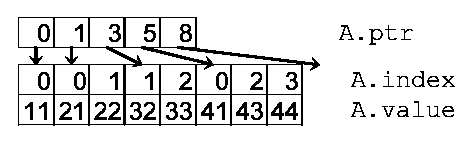
\includegraphics{storage01.eps} 
\end{flushleft}
\end{minipage}
\caption{The data structure of the CRS format (for serial and OpenMP versions).}\label{fig:storage01}}
\end{figure}
\begin{itembox}[l]{for serial and OpenMP versions}
\small
\begin{verbatim}
 1: int           n,nnz;
 2: int           *ptr,*index;
 3: LIS_SCALAR    *value;
 4: LIS_MATRIX    A;
 5: n = 4; nnz = 8;
 6: ptr   = (int *)malloc( (n+1)*sizeof(int) );
 7: index = (int *)malloc( nnz*sizeof(int) );
 8: value = (LIS_SCALAR *)malloc( nnz*sizeof(LIS_SCALAR) );
 9: lis_matrix_create(0,&A);
10: lis_matrix_set_size(A,0,n);
11:
12: ptr[0] = 0; ptr[1] = 1; ptr[2] = 3; ptr[3] = 5; ptr[4] = 8;
13: index[0] =  0; index[1] =  0; index[2] =  1; index[3] =  1;
14: index[4] =  2; index[5] =  0; index[6] =  2; index[7] =  3;
15: value[0] = 11; value[1] = 21; value[2] = 22; value[3] = 32;
16: value[4] = 33; value[5] = 41; value[6] = 43; value[7] = 44;
17:
18:  lis_matrix_set_crs(nnz,ptr,index,value,A);
19:  lis_matrix_assemble(A);
\end{verbatim}
\end{itembox}
\subsubsection{Creating Matrices (for MPI Version)}
Figure \ref{fig:storage01_mpi} shows how the matrix $A$ in 
Figure \ref{fig:storage01} is stored in the CRS format on two 
processing elements. A program to create the matrix in the CRS format 
on two processing elements is as follows:
\begin{figure}[h]
{\centering 
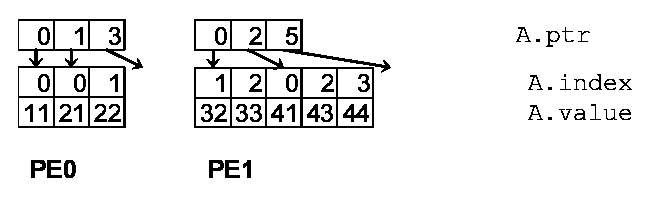
\includegraphics{storage01_mpi.eps} 
\caption{The data structure of the CRS format (for MPI version).}\label{fig:storage01_mpi}}
\end{figure}
\begin{itembox}[l]{for MPI version}
\small
\begin{verbatim}
 1: int           i,k,n,nnz,my_rank;
 2: int           *ptr,*index;
 3: LIS_SCALAR    *value;
 4: LIS_MATRIX    A;
 5: MPI_Comm_rank(MPI_COMM_WORLD,&my_rank);
 6: if( my_rank==0 ) {n = 2; nnz = 3;}
 7: else             {n = 2; nnz = 5;}
 8: ptr   = (int *)malloc( (n+1)*sizeof(int) );
 9: index = (int *)malloc( nnz*sizeof(int) );
10: value = (LIS_SCALAR *)malloc( nnz*sizeof(LIS_SCALAR) );
11: lis_matrix_create(MPI_COMM_WORLD,&A);
12: lis_matrix_set_size(A,n,0);
13: if( my_rank==0 ) {
14:     ptr[0] = 0; ptr[1] = 1; ptr[2] = 3;
15:     index[0] =  0; index[1] =  0; index[2] =  1;
16:     value[0] = 11; value[1] = 21; value[2] = 22;}
17: else {
18:     ptr[0] = 0; ptr[1] = 2; ptr[2] = 5;
19:     index[0] =  1; index[1] =  2; index[2] =  0; index[3] =  2; index[4] =  3;
20:     value[0] = 32; value[1] = 33; value[2] = 41; value[3] = 43; value[4] = 44;}
21:  lis_matrix_set_crs(nnz,ptr,index,value,A);
22:  lis_matrix_assemble(A);
\end{verbatim}
\end{itembox}
\subsubsection{Associating Arrays}
To associate the arrays required by the CRS format with the matrix $A$, the following functions are used:
\begin{itemize}
\item \verb|C       int lis_matrix_set_crs(int nnz, int row[], int index[], LIS_SCALAR value[],|\\
      \verb| LIS_MATRIX A)|
\item \verb|Fortran subroutine lis_matrix_set_crs(integer nnz, integer row(), integer index(),|\\
      \verb| LIS_SCALAR value(), LIS_MATRIX A, integer ierr)|
\end{itemize}
%%%%%%%%%%%%%%%%%%%%%%%%%%%%%%%%%%%%%%%%%%%%%%%%%%%%%%%%%%%%%%%%%%
% Compressed Column Storage (CCS)
%%%%%%%%%%%%%%%%%%%%%%%%%%%%%%%%%%%%%%%%%%%%%%%%%%%%%%%%%%%%%%%%%%
\newpage
\subsection{Compressed Column Storage (CCS)}
The CSS format uses three arrays {\ttfamily ptr}, {\ttfamily index} and
{\ttfamily value} to store data.
\begin{itemize}
\item {\ttfamily value} is a double precision array with a length of
      $nnz$, which stores the values for the nonzero elements of the matrix $A$ along the column.
\item {\ttfamily index} is an integer array with a length of $nnz$, which
      stores the row numbers of the nonzero elements stored in the
      array {\ttfamily value}.
\item {\ttfamily ptr} is an integer array with a length of $n+1$, which
      stores the starting points of the rows of the arrays {\ttfamily value} and {\ttfamily index}. 
\end{itemize}

\subsubsection{Creating Matrices (for Serial and OpenMP Versions)}
The right diagram in Figure \ref{fig:storage02} shows how the matrix $A$ in Figure \ref{fig:storage02} is stored in the CCS format. A program to create the matrix in the CCS format is as follows:

\begin{figure}[h]
{\centering 
\begin{minipage}{0.3\textwidth}
\begin{flushright}
$ 
A = \left(
\begin{array}{cccc}
11 &    &    &    \\
21 & 22 &    &    \\
   & 32 & 33 &    \\
41 &    & 43 & 44 \\
\end{array}\right)
$
\end{flushright}
\end{minipage}
\begin{minipage}{0.6\textwidth}
\begin{flushleft}
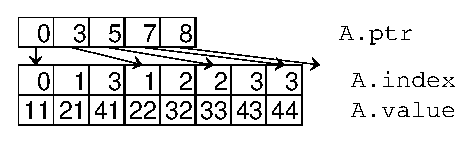
\includegraphics{storage02.eps} 
\end{flushleft}
\end{minipage}
\caption{The data structure of the CCS format (for serial and OpenMP versions).}\label{fig:storage02}}
\end{figure}
\begin{itembox}[l]{for serial and OpenMP versions}
\small
\begin{verbatim}
 1: int           n,nnz;
 2: int           *ptr,*index;
 3: LIS_SCALAR    *value;
 4: LIS_MATRIX    A;
 5: n = 4; nnz = 8;
 6: ptr   = (int *)malloc( (n+1)*sizeof(int) );
 7: index = (int *)malloc( nnz*sizeof(int) );
 8: value = (LIS_SCALAR *)malloc( nnz*sizeof(LIS_SCALAR) );
 9: lis_matrix_create(0,&A);
10: lis_matrix_set_size(A,0,n);
11:
12: ptr[0] = 0; ptr[1] = 3; ptr[2] = 5; ptr[3] = 7; ptr[4] = 8;
13: index[0] =  0; index[1] =  1; index[2] =  3; index[3] =  1;
14: index[4] =  2; index[5] =  2; index[6] =  3; index[7] =  3;
15: value[0] = 11; value[1] = 21; value[2] = 41; value[3] = 22;
16: value[4] = 32; value[5] = 33; value[6] = 43; value[7] = 44;
17:
18:  lis_matrix_set_ccs(nnz,ptr,index,value,A);
19:  lis_matrix_assemble(A);
\end{verbatim}
\end{itembox}
\newpage
\subsubsection{Creating Matrices (for MPI Version)}
Figure \ref{fig:storage02_mpi} shows how the matrix $A$ in Figure
\ref{fig:storage02} is stored on two processing elements. A program to create the
matrix in the CCS format on two processing elements is as follows:
\begin{figure}[h]
{\centering 
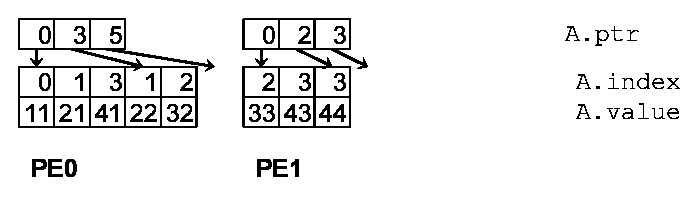
\includegraphics{storage02_mpi.eps} 
\caption{The data structure of the CCS format (for MPI version).}\label{fig:storage02_mpi}}
\end{figure}
\begin{itembox}[l]{for MPI version}
\small
\begin{verbatim}
 1: int           i,k,n,nnz,my_rank;
 2: int           *ptr,*index;
 3: LIS_SCALAR    *value;
 4: LIS_MATRIX    A;
 5: MPI_Comm_rank(MPI_COMM_WORLD,&my_rank);
 6: if( my_rank==0 ) {n = 2; nnz = 3;}
 7: else             {n = 2; nnz = 5;}
 8: ptr   = (int *)malloc( (n+1)*sizeof(int) );
 9: index = (int *)malloc( nnz*sizeof(int) );
10: value = (LIS_SCALAR *)malloc( nnz*sizeof(LIS_SCALAR) );
11: lis_matrix_create(MPI_COMM_WORLD,&A);
12: lis_matrix_set_size(A,n,0);
13: if( my_rank==0 ) {
14:     ptr[0] = 0; ptr[1] = 3; ptr[2] = 5;
15:     index[0] =  0; index[1] =  1; index[2] =  3; index[3] =  1; index[4] =  2;
16:     value[0] = 11; value[1] = 21; value[2] = 41; value[3] = 22; value[4] = 32}
17: else {
18:     ptr[0] = 0; ptr[1] = 2; ptr[2] = 3;
19:     index[0] =  2; index[1] =  3; index[2] =  3;
20:     value[0] = 33; value[1] = 43; value[2] = 44;}
21:  lis_matrix_set_ccs(nnz,ptr,index,value,A);
22:  lis_matrix_assemble(A);
\end{verbatim}
\end{itembox}
\subsubsection{Associating Arrays}
To associate the arrays required by the CCS format with the matrix $A$, the following functions are used:
\begin{itemize}
\item \verb|C       int lis_matrix_set_ccs(int nnz, int row[], int index[], LIS_SCALAR value[],|\\
\item \verb|Fortran subroutine lis_matrix_set_ccs(integer nnz, integer row(), integer index(),|\\
      \verb| LIS_SCALAR value(), LIS_MATRIX A, integer ierr)|
\end{itemize}

%%%%%%%%%%%%%%%%%%%%%%%%%%%%%%%%%%%%%%%%%%%%%%%%%%%%%%%%%%%%%%%%%%
% Modified Compressed Sparse Row (MSR)
%%%%%%%%%%%%%%%%%%%%%%%%%%%%%%%%%%%%%%%%%%%%%%%%%%%%%%%%%%%%%%%%%%
\newpage
\subsection{Modified Compressed Sparse Row (MSR)}
The MSR format is a modified version of the CRS format. 
The MSR format is different in that it separates the diagonal elements before storing it. 
The MSR format uses two arrays {\ttfamily index} and {\ttfamily value} to store data. 
Assume that $ndz$ represents the number of the zero elements of the diagonal.
\begin{itemize}
\item {\ttfamily value} is a double precision array with a length of
      $nnz+ndz+1$, which stores the diagonal of the matrix A down to the
      $n$-th element. The $n+1$-th element is not used. For the $n+2$-th
      and after, the values of the nonzero elements except the diagonal of the matrix $A$ are stored along the row.
\item {\ttfamily index} is an integer array with a length of
      $nnz+ndz+1$, 
      which stores the starting points of the rows of the off-diagonal
      elements of the matrix $A$ down to the $n+1$-th element. For the
      $n+2$-th and after, 
      it stores the row numbers of the off-diagonal elements of
      the matrix $A$ stored in the array {\ttfamily value}.
\end{itemize}

\subsubsection{Creating Matrices (for Serial and OpenMP Versions)}
The right diagram in Figure \ref{fig:storage03} shows how matrix A is stored in the MSR format. A program to create the matrix in the MSR format is as follows:
\begin{figure}[h]
{\centering 
\begin{minipage}{0.3\textwidth}
\begin{flushright}
$ 
A = \left(
\begin{array}{cccc}
11 &    &    &    \\
21 & 22 &    &    \\
   & 32 & 33 &    \\
41 &    & 43 & 44 \\
\end{array}\right)
$
\end{flushright}
\end{minipage}
\begin{minipage}{0.6\textwidth}
\begin{flushleft}
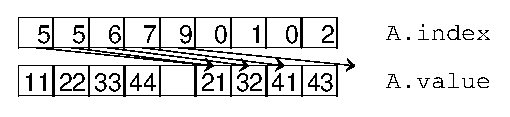
\includegraphics{storage03.eps} 
\end{flushleft}
\end{minipage}
\caption{The data structure of the MSR format (for serial and OpenMP versions).}\label{fig:storage03}}
\end{figure}
\begin{itembox}[l]{for serial and OpenMP versions}
\small
\begin{verbatim}
 1: int           n,nnz,ndz;
 2: int           *index;
 3: LIS_SCALAR    *value;
 4: LIS_MATRIX    A;
 5: n = 4; nnz = 8; ndz = 0;
 6: index = (int *)malloc( (nnz+ndz+1)*sizeof(int) );
 7: value = (LIS_SCALAR *)malloc( (nnz+ndz+1)*sizeof(LIS_SCALAR) );
 8: lis_matrix_create(0,&A);
 9: lis_matrix_set_size(A,0,n);
10:
11: index[0] =  5; index[1] =  5; index[2] =  6; index[3] =  7;
12: index[4] =  9; index[5] =  0; index[6] =  1; index[7] =  0; index[8] =  2;
13: value[0] = 11; value[1] = 22; value[2] = 33; value[3] = 44;
14: value[4] =  0; value[5] = 21; value[6] = 32; value[7] = 41; value[8] = 43;
15:
16:  lis_matrix_set_msr(nnz,ndz,index,value,A);
17:  lis_matrix_assemble(A);
\end{verbatim}
\end{itembox}
\newpage
\subsubsection{Creating Matrices (for MPI Version)}
Figure \ref{fig:storage03_mpi} shows how the matrix $A$ in Figure
\ref{fig:storage03} is stored in the MSR format on two processing 
elements. A program to create the matrix in the MSR format on two processing element is as follows:
\begin{figure}[h]
{\centering 
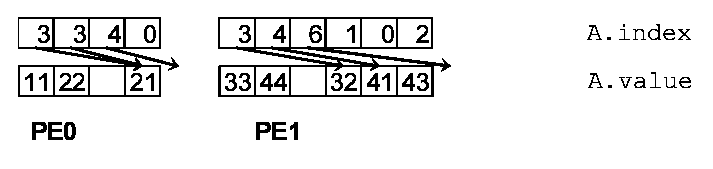
\includegraphics{storage03_mpi.eps} 
\caption{The data structure of the MSR format (for MPI version).}\label{fig:storage03_mpi}}
\end{figure}
\begin{itembox}[l]{for MPI version}
\small
\begin{verbatim}
 1: int           i,k,n,nnz,ndz,my_rank;
 2: int           *index;
 3: LIS_SCALAR    *value;
 4: LIS_MATRIX    A;
 5: MPI_Comm_rank(MPI_COMM_WORLD,&my_rank);
 6: if( my_rank==0 ) {n = 2; nnz = 3; ndz = 0;}
 7: else             {n = 2; nnz = 5; ndz = 0;}
 8: index = (int *)malloc( (nnz+ndz+1)*sizeof(int) );
 9: value = (LIS_SCALAR *)malloc( (nnz+ndz+1)*sizeof(LIS_SCALAR) );
10: lis_matrix_create(MPI_COMM_WORLD,&A);
11: lis_matrix_set_size(A,n,0);
12: if( my_rank==0 ) {
13:     index[0] =  3; index[1] =  3; index[2] =  4; index[3] =  0;
14:     value[0] = 11; value[1] = 22; value[2] =  0; value[3] = 21;}
15: else {
16:     index[0] =  3; index[1] =  4; index[2] =  6; index[3] =  1;
17:     index[4] =  0; index[5] =  2;
18:     value[0] = 33; value[1] = 44; value[2] =  0; value[3] = 32;
19:     value[4] = 41; value[5] = 43;}
20:  lis_matrix_set_msr(nnz,ndz,index,value,A);
21:  lis_matrix_assemble(A);
\end{verbatim}
\end{itembox}
\subsubsection{Associating Arrays}
To associate the arrays required by the MSR format with the matrix $A$, the following functions are used:
\begin{itemize}
\item \verb|C       int lis_matrix_set_msr(int nnz, int ndz, int index[], LIS_SCALAR value[], |\\
      \verb|LIS_MATRIX A)|
\item \verb|Fortran subroutine lis_matrix_set_msr(integer nnz, integer ndz, integer index(),|\\
      \verb| LIS_SCALAR value(), LIS_MATRIX A, integer ierr)|
\end{itemize}

%%%%%%%%%%%%%%%%%%%%%%%%%%%%%%%%%%%%%%%%%%%%%%%%%%%%%%%%%%%%%%%%%%
% Diagonal (DIA)
%%%%%%%%%%%%%%%%%%%%%%%%%%%%%%%%%%%%%%%%%%%%%%%%%%%%%%%%%%%%%%%%%%
\newpage
\subsection{Diagonal (DIA)}
DIA uses two arrays {\ttfamily index} and {\ttfamily value} to store
data. Assume that $nnd$ represents the number of the nonzero diagonal
elements of the matrix $A$.
\begin{itemize}
\item {\ttfamily value} is a double precision array with a length of
      $nnd \times n$, which stores nonzero diagonal elements of the matrix $A$.
\item {\ttfamily index} is an integer array with a length of $nnd$,
      which stores the offsets from the main diagonal.
\end{itemize}

For the OpenMP version, the following modifications have been made:
DIA uses two arrays {\ttfamily index} and {\ttfamily value} to store
data. Assume that $nprocs$ represents the number of the threads.
$nnd_p$ is the number of the nonzero diagonal elements of the partial matrix into which the row block of the matrix $A$ is divided.
$maxnnd$ is the maximum value $nnd_p$.
\begin{itemize}
\item {\ttfamily value} is a double precision array with a length of
      $maxnnd \times n$, which stores nonzero diagonal elements of the matrix $A$.
\item {\ttfamily index} is an integer array with a length of $nprocs
      \times maxnnd$, which stores the offsets from the main diagonal.
\end{itemize}

\subsubsection{Creating Matrices (for Serial Version)}
The right diagram in Figure \ref{fig:storage04} shows how the matrix $A$
in Figure \ref{fig:storage04} is stored in the DIA format. A program to create the matrix in the DIA format is as follows:
\begin{figure}[h]
{\centering 
\begin{minipage}{0.3\textwidth}
\begin{flushright}
$ 
A = \left(
\begin{array}{cccc}
11 &    &    &    \\
21 & 22 &    &    \\
   & 32 & 33 &    \\
41 &    & 43 & 44 \\
\end{array}\right)
$
\end{flushright}
\end{minipage}
\begin{minipage}{0.6\textwidth}
\begin{flushleft}
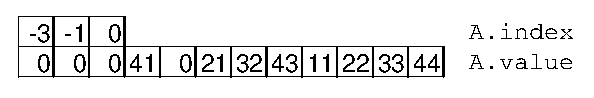
\includegraphics{storage04.eps} 
\end{flushleft}
\end{minipage}
\caption{The data structure of the DIA format (for serial version).}\label{fig:storage04}}
\end{figure}
\begin{itembox}[l]{for serial version}
\small
\begin{verbatim}
 1: int           n,nnd;
 2: int           *index;
 3: LIS_SCALAR    *value;
 4: LIS_MATRIX    A;
 5: n = 4; nnd = 3;
 6: index = (int *)malloc( nnd*sizeof(int) );
 7: value = (LIS_SCALAR *)malloc( n*nnd*sizeof(LIS_SCALAR) );
 8: lis_matrix_create(0,&A);
 9: lis_matrix_set_size(A,0,n);
10:
11: index[0] = -3; index[1] = -1; index[2] =  0;
12: value[0] =  0; value[1] =  0; value[2] =  0; value[3] = 41;
13: value[4] =  0; value[5] = 21; value[6] = 32; value[7] = 43;
14: value[8] = 11; value[9] = 22; value[10]= 33; value[11]= 44;
15:
16:  lis_matrix_set_dia(nnd,index,value,A);
17:  lis_matrix_assemble(A);
\end{verbatim}
\end{itembox}
\newpage
\subsubsection{Creating Matrices (for OpenMP Version)}
Figure \ref{fig:storage04_omp} shows how the matrix $A$ in Figure \ref{fig:storage04} is stored in the DIA format on two threads. A program to create the matrix in the DIA format on two threads is as follows:
\begin{figure}[h]
{\centering 
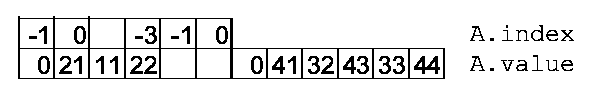
\includegraphics{storage04_omp.eps} 
\caption{The data structure of the DIA format (for OpenMP version).}\label{fig:storage04_omp}}
\end{figure}
\begin{itembox}[l]{for OpenMP version}
\small
\begin{verbatim}
 1: int           n,maxnnd,nprocs;
 2: int           *index;
 3: LIS_SCALAR    *value;
 4: LIS_MATRIX    A;
 5: n = 4; maxnnd = 3; nprocs = 2;
 6: index = (int *)malloc( maxnnd*sizeof(int) );
 7: value = (LIS_SCALAR *)malloc( n*maxnnd*sizeof(LIS_SCALAR) );
 8: lis_matrix_create(0,&A);
 9: lis_matrix_set_size(A,0,n);
10:
11: index[0] = -1; index[1] =  0; index[2] =  0; index[3] = -3; index[4] = -1; index[5] =  0;
12: value[0] =  0; value[1] = 21; value[2] = 11; value[3] = 22; value[4] =  0; value[5] =  0;
13: value[6] =  0; value[7] = 41; value[8] = 32; value[9] = 43; value[10]= 33; value[11]= 44;
14:
15:  lis_matrix_set_dia(maxnnd,index,value,A);
16:  lis_matrix_assemble(A);
\end{verbatim}
\end{itembox}
\newpage
\subsubsection{Creating Matrices (for MPI Version)}
Figure \ref{fig:storage04_mpi} shows how the matrix $A$ in Figure \ref{fig:storage04} is stored in the DIA format on two processing elements. A program to create the matrix in the DIA format on two processing elements is as follows:
\begin{figure}[h]
{\centering 
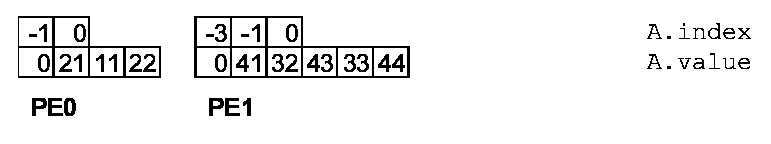
\includegraphics{storage04_mpi.eps} 
\caption{The data structure of the DIA format (for MPI version).}\label{fig:storage04_mpi}}
\end{figure}
\begin{itembox}[l]{for MPI version}
\small
\begin{verbatim}
 1: int           i,n,nnd,my_rank;
 2: int           *index;
 3: LIS_SCALAR    *value;
 4: LIS_MATRIX    A;
 5: MPI_Comm_rank(MPI_COMM_WORLD,&my_rank);
 6: if( my_rank==0 ) {n = 2; nnd = 2;}
 7: else             {n = 2; nnd = 3;}
 8: index = (int *)malloc( nnd*sizeof(int) );
 9: value = (LIS_SCALAR *)malloc( n*nnd*sizeof(LIS_SCALAR) );
10: lis_matrix_create(MPI_COMM_WORLD,&A);
11: lis_matrix_set_size(A,n,0);
12: if( my_rank==0 ) {
13:     index[0] = -1; index[1] =  0;
14:     value[0] =  0; value[1] = 21; value[2] = 11; value[3] = 22;}
15: else {
16:     index[0] = -3; index[1] = -1; index[2] =  0;
17:     value[0] =  0; value[1] = 41; value[2] = 32; value[3] = 43; value[4] = 33;
18:     value[5] = 44;}
19:  lis_matrix_set_dia(nnd,index,value,A);
20:  lis_matrix_assemble(A);
\end{verbatim}
\end{itembox}
\subsubsection{Associating Arrays}
To associate the arrays required by the DIA format with the matrix $A$, the following functions are used:
\begin{itemize}
\item \verb|C       int lis_matrix_set_dia(int nnd, int index[], LIS_SCALAR value[], LIS_MATRIX A)|
\item \verb|Fortran subroutine lis_matrix_set_dia(integer nnd, integer index(), LIS_SCALAR value(),|\\
      \verb| LIS_MATRIX A, integer ierr)|
\end{itemize}

%%%%%%%%%%%%%%%%%%%%%%%%%%%%%%%%%%%%%%%%%%%%%%%%%%%%%%%%%%%%%%%%%%
% Ellpack-Itpack generalized diagonal (ELL)
%%%%%%%%%%%%%%%%%%%%%%%%%%%%%%%%%%%%%%%%%%%%%%%%%%%%%%%%%%%%%%%%%%
\newpage
\subsection{Ellpack-Itpack generalized diagonal (ELL)}
ELL uses two arrays {\ttfamily index} and {\ttfamily value} to store
data. Assume that $maxnzr$ is the maximum value for the number of the nonzero elements in the rows of the matrix $A$.
\begin{itemize}
\item {\ttfamily value} is a double precision array with a length of
      $maxnzr \times n$, which stores the nonzero elements of the rows
      of the matrix $A$ along the column. The first column consists of
      the first nonzero elements of each row. If there is no nonzero elements to be stored, then $0$ is stored.
\item {\ttfamily index} is an integer array with a length of $maxnzr
      \times n$, which stores the column numbers of the nonzero
      elements stored in the array {\ttfamily value}. If the number of
      the nonzero elements in the $i$-th row is $nnz$, then {\tt index[$nnz
      \times n + i$]} stores row number $i$.
\end{itemize}

\subsubsection{Creating Matrices (for Serial and OpenMP Versions)}
The right diagram in Figure \ref{fig:storage05} shows how the matrix $A$ in Figure \ref{fig:storage05} is stored in the ELL format. A program to create the matrix in the ELL format is as follows:
\begin{figure}[h]
{\centering 
\begin{minipage}{0.3\textwidth}
\begin{flushright}
$ 
A = \left(
\begin{array}{cccc}
11 &    &    &    \\
21 & 22 &    &    \\
   & 32 & 33 &    \\
41 &    & 43 & 44 \\
\end{array}\right)
$
\end{flushright}
\end{minipage}
\begin{minipage}{0.6\textwidth}
\begin{flushleft}
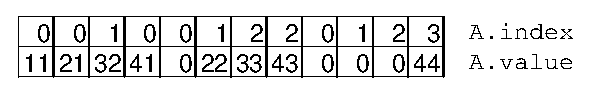
\includegraphics{storage05.eps} 
\end{flushleft}
\end{minipage}
\caption{The data structure of the ELL format (for serial and OpenMP versions).}\label{fig:storage05}}
\end{figure}
\begin{itembox}[l]{for serial and OpenMP versions}
\small
\begin{verbatim}
 1: int           n,maxnzr;
 2: int           *index;
 3: LIS_SCALAR    *value;
 4: LIS_MATRIX    A;
 5: n = 4; maxnzr = 3;
 6: index = (int *)malloc( n*maxnzr*sizeof(int) );
 7: value = (LIS_SCALAR *)malloc( n*maxnzr*sizeof(LIS_SCALAR) );
 8: lis_matrix_create(0,&A);
 9: lis_matrix_set_size(A,0,n);
10:
11: index[0] =  0; index[1] =  0; index[2] =  1; index[3] =  0; index[4] =  0; index[5] =  1;
12: index[6] =  2; index[7] =  2; index[8] =  0; index[9] =  1; index[10]=  2; index[11]=  3;
13: value[0] = 11; value[1] = 21; value[2] = 32; value[3] = 41; value[4] =  0; value[5] = 22;
14: value[6] = 33; value[7] = 43; value[8] =  0; value[9] =  0; value[10]=  0; value[11]= 44;
15:
16:  lis_matrix_set_ell(maxnzr,index,value,A);
17:  lis_matrix_assemble(A);
\end{verbatim}
\end{itembox}
\newpage
\subsubsection{Creating Matrices (for MPI Version)}
Figure \ref{fig:storage05_mpi} shows how the matrix $A$ in Figure \ref{fig:storage05} is stored in the ELL format. A program to create the matrix in the ELL format on two processing elements is as follows:
\begin{figure}[h]
{\centering 
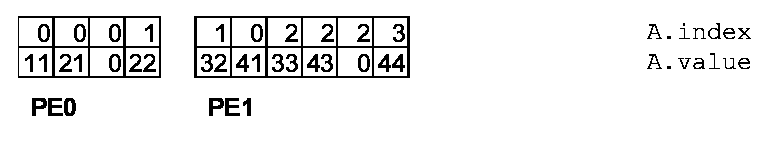
\includegraphics{storage05_mpi.eps} 
\caption{The data structure of the ELL format (for MPI version).}\label{fig:storage05_mpi}}
\end{figure}
\begin{itembox}[l]{for MPI version}
\small
\begin{verbatim}
 1: int           i,n,maxnzr,my_rank;
 2: int           *index;
 3: LIS_SCALAR    *value;
 4: LIS_MATRIX    A;
 5: MPI_Comm_rank(MPI_COMM_WORLD,&my_rank);
 6: if( my_rank==0 ) {n = 2; maxnzr = 2;}
 7: else             {n = 2; maxnzr = 3;}
 8: index = (int *)malloc( n*maxnzr*sizeof(int) );
 9: value = (LIS_SCALAR *)malloc( n*maxnzr*sizeof(LIS_SCALAR) );
10: lis_matrix_create(MPI_COMM_WORLD,&A);
11: lis_matrix_set_size(A,n,0);
12: if( my_rank==0 ) {
13:     index[0] =  0; index[1] =  0; index[2] =  0; index[3] =  1;
14:     value[0] = 11; value[1] = 21; value[2] =  0; value[3] = 22;}
15: else {
16:     index[0] =  1; index[1] =  0; index[2] =  2; index[3] =  2; index[4] =  2;
17:     index[5] =  3;
18:     value[0] = 32; value[1] = 41; value[2] = 33; value[3] = 43; value[4] =  0;
19:     value[5] = 44;}
20:  lis_matrix_set_ell(maxnzr,index,value,A);
21:  lis_matrix_assemble(A);
\end{verbatim}
\end{itembox}
\subsubsection{Associating Arrays}
To associate an array required by the ELL format with the matrix $A$, the following functions are used:
\begin{itemize}
\item \verb|C       int lis_matrix_set_ell(int maxnzr, int index[], LIS_SCALAR value[],|\\
      \verb| LIS_MATRIX A)|
\item \verb|Fortran subroutine lis_matrix_set_ell(integer maxnzr, integer index(),|\\
      \verb| LIS_SCALAR value(), LIS_MATRIX A, integer ierr)|
\end{itemize}

%%%%%%%%%%%%%%%%%%%%%%%%%%%%%%%%%%%%%%%%%%%%%%%%%%%%%%%%%%%%%%%%%%
% Jagged Diagonal (JDS)
%%%%%%%%%%%%%%%%%%%%%%%%%%%%%%%%%%%%%%%%%%%%%%%%%%%%%%%%%%%%%%%%%%
\newpage
\subsection{Jagged Diagonal (JDS)}
JDS first sorts the nonzero elements of the rows in decreasing order of
size, and then stores them along the column. JDS uses four arrays
{\ttfamily perm}, {\ttfamily ptr}, {\ttfamily index} and {\ttfamily
value} to store date. Assume that $maxnzr$ represents the maximum value
of the number of the nonzero elements of the matrix $A$.
\begin{itemize}
\item {\ttfamily perm} is an integer array with a length of $n$, which stores the sorted row numbers.
\item {\ttfamily value} is a double precision array with a length of
      $nnz$, which stores the jagged diagonal elements of the sorted matrix $A$. The
      first jagged diagonal consists of the first nonzero elements of
      each row. The next jagged diagonal consists of the second nonzero 
      elements, and so on. 
\item {\ttfamily index} is an integer array with a length of $nnz$,
      which stores the row numbers of the nonzero elements stored in
      the array {\ttfamily value}.
\item {\ttfamily ptr} is an integer array with a length of $maxnzr+1$,
      which stores the starting points of the jagged diagonal elements.
\end{itemize}

For the OpenMP version, the following modifications have been made:
JDS uses four arrays {\ttfamily perm}, {\ttfamily ptr}, {\ttfamily
index} and {\ttfamily value} to store data. Assume that $nprocs$ is the
number of the threads.
$maxnzr_p$ is the number of the nonzero diagonal elements of the partial matrix into which the row block of the matrix $A$ is divided.
$maxmaxnzr$ is the maximum value of $maxnzr_p$.
\begin{itemize}
\item {\ttfamily perm} is an integer array with a length of $n$, which stores the sorted row numbers.
\item {\ttfamily value} is a double precision array with a length of
      $nnz$, which stores jagged diagonal elements of the sorted matrix $A$. The
      first jagged diagonal consists of the first nonzero elements of
      each row. The next jagged diagonal consist of the second
      nonzero elements of each row, and so on. 
\item {\ttfamily index} is an integer array with a length of $nnz$,
      which stores the row numbers of the nonzero elements stored in
      the array {\ttfamily value}.
\item {\ttfamily ptr} is an integer array with a length of $nprocs
      \times (maxmaxnzr + 1)$, which stores the starting points of the
      jagged diagonal elements.
\end{itemize}

\newpage
\subsubsection{Creating Matrices (for Serial Version)}
The right diagram in Figure \ref{fig:storage06} shows how the matrix $A$ in Figure \ref{fig:storage06} is stored in the JDS format. A program to create the matrix in the JDS format is as follows: 
\begin{figure}[h]
{\centering 
\begin{minipage}{0.3\textwidth}
\begin{flushright}
$ 
A = \left(
\begin{array}{cccc}
11 &    &    &    \\
21 & 22 &    &    \\
   & 32 & 33 &    \\
41 &    & 43 & 44 \\
\end{array}\right)
$
\end{flushright}
\end{minipage}
\begin{minipage}{0.6\textwidth}
\begin{flushleft}
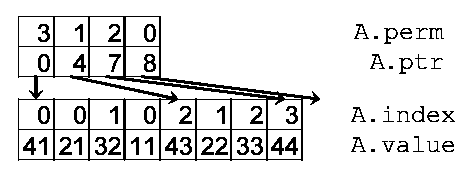
\includegraphics{storage06.eps} 
\end{flushleft}
\end{minipage}
\caption{The data structure of the JDS format (for serial version).}\label{fig:storage06}}
\end{figure}
\begin{itembox}[l]{for serial version}
\small
\begin{verbatim}
 1: int           n,nnz,maxnzr;
 2: int           *perm,*ptr,*index;
 3: LIS_SCALAR    *value;
 4: LIS_MATRIX    A;
 5: n = 4; nnz = 8; maxnzr = 3;
 6: perm  = (int *)malloc( n*sizeof(int) );
 7: ptr   = (int *)malloc( (maxnzr+1)*sizeof(int) );
 8: index = (int *)malloc( nnz*sizeof(int) );
 9: value = (LIS_SCALAR *)malloc( nnz*sizeof(LIS_SCALAR) );
10: lis_matrix_create(0,&A);
11: lis_matrix_set_size(A,0,n);
12:
13: perm[0] = 3; perm[1] = 1; perm[2] = 2; perm[3] = 0;
14: ptr[0]  = 0; ptr[1]  = 4; ptr[2]  = 7; ptr[3]  = 8;
15: index[0] =  0; index[1] =  0; index[2] =  1; index[3] =  0;
16: index[4] =  2; index[5] =  1; index[6] =  2; index[7] =  3;
17: value[0] = 41; value[1] = 21; value[2] = 32; value[3] = 11;
18: value[4] = 43; value[5] = 22; value[6] = 33; value[7] = 44;
19:
20:  lis_matrix_set_jds(nnz,maxnzr,perm,ptr,index,value,A);
21:  lis_matrix_assemble(A);
\end{verbatim}
\end{itembox}
\newpage
\subsubsection{Creating Matrices (for OpenMP Version)}
Figure \ref{fig:storage06_omp} shows how the matrix $A$ in Figure \ref{fig:storage06} is stored in the JDS format on two threads. A program to create the matrix in the JDS format on two threads is as follows:
\begin{figure}[h]
{\centering 
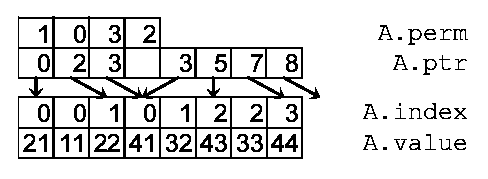
\includegraphics{storage06_omp.eps} 
\caption{The data structure of the JDS format (for OpenMP version).}\label{fig:storage06_omp}}
\end{figure}
\begin{itembox}[l]{for OpenMP version}
\small
\begin{verbatim}
 1: int           n,nnz,maxmaxnzr,nprocs;
 2: int           *perm,*ptr,*index;
 3: LIS_SCALAR    *value;
 4: LIS_MATRIX    A;
 5: n = 4; nnz = 8; maxmaxnzr = 3; nprocs = 2;
 6: perm  = (int *)malloc( n*sizeof(int) );
 7: ptr   = (int *)malloc( nprocs*(maxmaxnzr+1)*sizeof(int) );
 8: index = (int *)malloc( nnz*sizeof(int) );
 9: value = (LIS_SCALAR *)malloc( nnz*sizeof(LIS_SCALAR) );
10: lis_matrix_create(0,&A);
11: lis_matrix_set_size(A,0,n);
12:
13: perm[0] = 1; perm[1] = 0; perm[2] = 3; perm[3] = 2;
14: ptr[0]  = 0; ptr[1]  = 2; ptr[2]  = 3; ptr[3]  = 0;
15: ptr[4]  = 3; ptr[5]  = 5; ptr[6]  = 7; ptr[7]  = 8;
16: index[0] =  0; index[1] =  0; index[2] =  1; index[3] =  0;
17: index[4] =  1; index[5] =  2; index[6] =  2; index[7] =  3;
18: value[0] = 21; value[1] = 11; value[2] = 22; value[3] = 41;
19: value[4] = 32; value[5] = 43; value[6] = 33; value[7] = 44;
20:
21:  lis_matrix_set_jds(nnz,maxmaxnzr,perm,ptr,index,value,A);
22:  lis_matrix_assemble(A);
\end{verbatim}
\end{itembox}
\newpage
\subsubsection{Creating Matrices (for MPI Version)}
Figure \ref{fig:storage06_mpi} shows how the matrix $A$ in Figure \ref{fig:storage06} is stored in the JDS format on two processing elements. A program to create the matrix in the JDS format on two processing elements is as follows:
\begin{figure}[h]
{\centering 
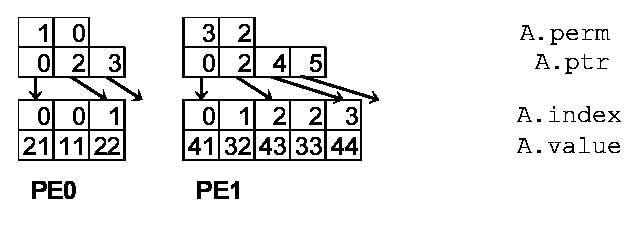
\includegraphics{storage06_mpi.eps} 
\caption{The data structure of the JDS format (for MPI version).}\label{fig:storage06_mpi}}
\end{figure}
\begin{itembox}[l]{for MPI version}
\small
\begin{verbatim}
 1: int           i,n,nnz,maxnzr,my_rank;
 2: int           *perm,*ptr,*index;
 3: LIS_SCALAR    *value;
 4: LIS_MATRIX    A;
 5: MPI_Comm_rank(MPI_COMM_WORLD,&my_rank);
 6: if( my_rank==0 ) {n = 2; nnz = 3; maxnzr = 2;}
 7: else             {n = 2; nnz = 5; maxnzr = 3;}
 8: perm  = (int *)malloc( n*sizeof(int) );
 9: ptr   = (int *)malloc( (maxnzr+1)*sizeof(int) );
10: index = (int *)malloc( nnz*sizeof(int) );
11: value = (LIS_SCALAR *)malloc( nnz*sizeof(LIS_SCALAR) );
12: lis_matrix_create(MPI_COMM_WORLD,&A);
13: lis_matrix_set_size(A,n,0);
14: if( my_rank==0 ) {
15:     perm[0] = 1; perm[1] = 0;
16:     ptr[0]  = 0; ptr[1]  = 2; ptr[2]  = 3;
17:     index[0] =  0; index[1] =  0; index[2] =  1;
18:     value[0] = 21; value[1] = 11; value[2] = 22;}
19: else {
20:     perm[0] = 3; perm[1] = 2;
21:     ptr[0]  = 0; ptr[1]  = 2; ptr[2]  = 4; ptr[3]  = 5;
22:     index[0] =  0; index[1] =  1; index[2] =  2; index[3] =  2; index[4] =  3;
23:     value[0] = 41; value[1] = 32; value[2] = 43; value[3] = 33; value[4] = 44;}
24:  lis_matrix_set_jds(nnz,maxnzr,perm,ptr,index,value,A);
25:  lis_matrix_assemble(A);
\end{verbatim}
\end{itembox}
\subsubsection{Associating Arrays}
To associate an array required by the JDS format with the matrix $A$, the following functions are used:
\begin{itemize}
\item \verb|C       int lis_matrix_set_jds(int nnz, int maxnzr, int perm[], int ptr[],|\\
      \verb| int index[], LIS_SCALAR value[], LIS_MATRIX A)|
\item \verb|Fortran subroutine lis_matrix_set_jds(integer nnz, integer maxnzr, integer ptr(),|\\
      \verb| integer index(), LIS_SCALAR value(), LIS_MATRIX A, integer ierr)|
\end{itemize}

%%%%%%%%%%%%%%%%%%%%%%%%%%%%%%%%%%%%%%%%%%%%%%%%%%%%%%%%%%%%%%%%%%
% Block Sparse Row (BSR)
%%%%%%%%%%%%%%%%%%%%%%%%%%%%%%%%%%%%%%%%%%%%%%%%%%%%%%%%%%%%%%%%%%
\newpage
\subsection{Block Sparse Row (BSR)}
BSR breaks down the matrix $A$ into partial matrices called blocks, with a size of $r \times c$. 
BSR stores nonzero blocks, in which at least one nonzero element exists, with the same step as that for the CRS format. 
Assume that $nr=n/r$ and $nnzb$ are the numbers of nonzero blocks of $A$. 
BSR uses three arrays {\ttfamily bptr}, {\ttfamily bindex} and {\ttfamily value} to store matrices.
\begin{itemize}
\item {\ttfamily value} is a double precision array with a length of
      $nnzb \times r \times c$, which stores all the elements of the nonzero blocks.
\item {\ttfamily bindex} is an integer array with a length of $nnzb$,
      which stores block column numbers of the nonzero blocks.
\item {\ttfamily bptr} is an integer array with a length of $nr+1$,
      which stores the starting points of the block rows in the array {\ttfamily bindex}.
\end{itemize}

\subsubsection{Creating Matrices (for Serial and OpenMP Versions)}
The right diagram in Figure \ref{fig:storage07} shows how the matrix $A$ in Figure \ref{fig:storage07} is stored in the BSR format. A program to create the matrix in the BSR format is as follows:
\begin{figure}[h]
{\centering 
\begin{minipage}{0.3\textwidth}
\begin{flushright}
$ 
A = \left(
\begin{array}{cc|cc}
11 &    &    &    \\
21 & 22 &    &    \\ \hline
   & 32 & 33 &    \\
41 &    & 43 & 44 \\
\end{array}\right)
$
\end{flushright}
\end{minipage}
\begin{minipage}{0.6\textwidth}
\begin{flushleft}
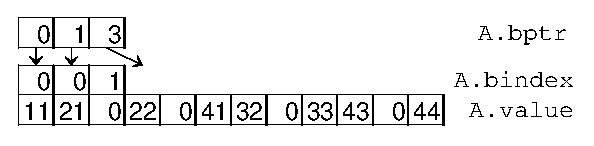
\includegraphics{storage07.eps} 
\end{flushleft}
\end{minipage}
\caption{The data structure of the BSR format (for serial and OpenMP versions).}\label{fig:storage07}}
\end{figure}
\begin{itembox}[l]{for serial and OpenMP versions}
\small
\begin{verbatim}
 1: int           n,bnr,bnc,nr,nc,bnnz;
 2: int           *bptr,*bindex;
 3: LIS_SCALAR    *value;
 4: LIS_MATRIX    A;
 5: n = 4; bnr = 2; bnc = 2; bnnz = 3; nr = (n-1)/bnr+1; nc = (n-1)/bnc+1;
 6: bptr   = (int *)malloc( (nr+1)*sizeof(int) );
 7: bindex = (int *)malloc( bnnz*sizeof(int) );
 8: value  = (LIS_SCALAR *)malloc( bnr*bnc*bnnz*sizeof(LIS_SCALAR) );
 9: lis_matrix_create(0,&A);
10: lis_matrix_set_size(A,0,n);
11:
12: bptr[0] = 0; bptr[1] = 1; bptr[2] = 3;
13: bindex[0] =  0; bindex[1] =  0; bindex[2] =  1;
14: value[0]  = 11; value[1] = 21; value[2] =  0; value[3] = 22;
15: value[4]  =  0; value[5] = 41; value[6] = 32; value[7] =  0;
16: value[8]  = 33; value[9] = 43; value[10]=  0; value[11]= 44;
17:
18:  lis_matrix_set_bsr(bnr,bnc,bnnz,bptr,bindex,value,A);
19:  lis_matrix_assemble(A);
\end{verbatim}
\end{itembox}
\newpage
\subsubsection{Creating Matrices (for MPI Version)}
Figure \ref{fig:storage07_mpi} shows how the matrix $A$ in Figure \ref{fig:storage07} is stored in the BSR format on two processing elements. A program to create the matrix in the BSR format on two processing elements is as follows:
\begin{figure}[h]
{\centering 
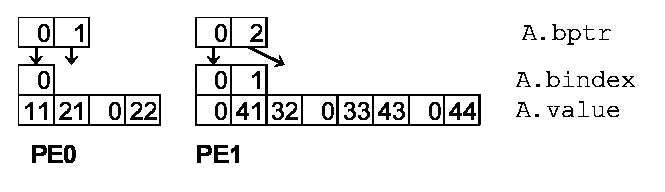
\includegraphics{storage07_mpi.eps} 
\caption{The data structure of the BSR format (for MPI version).}\label{fig:storage07_mpi}}
\end{figure}
\begin{itembox}[l]{for MPI version}
\small
\begin{verbatim}
 1: int           n,bnr,bnc,nr,nc,bnnz,my_rank;
 2: int           *bptr,*bindex;
 3: LIS_SCALAR    *value;
 4: LIS_MATRIX    A;
 5: MPI_Comm_rank(MPI_COMM_WORLD,&my_rank);
 6: if( my_rank==0 ) {n = 2; bnr = 2; bnc = 2; bnnz = 1; nr = (n-1)/bnr+1; nc = (n-1)/bnc+1;}
 7: else             {n = 2; bnr = 2; bnc = 2; bnnz = 2; nr = (n-1)/bnr+1; nc = (n-1)/bnc+1;}
 8: bptr   = (int *)malloc( (nr+1)*sizeof(int) );
 9: bindex = (int *)malloc( bnnz*sizeof(int) );
10: value  = (LIS_SCALAR *)malloc( bnr*bnc*bnnz*sizeof(LIS_SCALAR) );
11: lis_matrix_create(MPI_COMM_WORLD,&A);
12: lis_matrix_set_size(A,n,0);
13: if( my_rank==0 ) {
14:     bptr[0] = 0; bptr[1] = 1;
15:     bindex[0] =  0;
16:     value[0]  = 11; value[1] = 21; value[2] =  0; value[3] = 22;}
17: else {
18:     bptr[0] = 0; bptr[1] = 2;
19:     bindex[0] =  0; bindex[1] =  1;
20:     value[0]  =  0; value[1]  = 41; value[2] = 32; value[3] =  0;
21:     value[4]  = 33; value[5]  = 43; value[6] =  0; value[7] = 44;}
22:  lis_matrix_set_bsr(bnr,bnc,bnnz,bptr,bindex,value,A);
23:  lis_matrix_assemble(A);
\end{verbatim}
\end{itembox}
\subsubsection{Associating Arrays}
To associate the arrays required by the BSR format with the matrix $A$, the following functions are used:
\begin{itemize}
\item \verb|C       int lis_matrix_set_bsr(int bnr, int bnc, int bnnz, int bptr[],|\\
      \verb| int bindex[], LIS_SCALAR value[], LIS_MATRIX A)|
\item \verb|Fortran subroutine lis_matrix_set_bsr(integer bnr, integer bnc, integer bnnz,|\\
      \verb| integer bptr(), integer bindex(), LIS_SCALAR value(), LIS_MATRIX A, integer ierr)|
\end{itemize}

%%%%%%%%%%%%%%%%%%%%%%%%%%%%%%%%%%%%%%%%%%%%%%%%%%%%%%%%%%%%%%%%%%
% Block Sparse Column (BSC)
%%%%%%%%%%%%%%%%%%%%%%%%%%%%%%%%%%%%%%%%%%%%%%%%%%%%%%%%%%%%%%%%%%
\newpage
\subsection{Block Sparse Column (BSC)}
BSC breaks down the matrix $A$ into partial matrices called blocks, with a
size of $r \times c$. BSC stores nonzero blocks, in which at
least one nonzero block exists, in the same step as that for the CCS
format. Assume that $nc=n/c$ and $nnzb$ are the numbers of nonzero
blocks of A. BSC uses three arrays {\ttfamily bptr}, {\ttfamily bindex}
and {\ttfamily value} to store matrices. 
\begin{itemize}
\item {\ttfamily value} is a double precision array with a length of
      $nnzb \times r \times c$, which stores all the elements of the nonzero blocks.
\item {\ttfamily bindex} is an integer array with a length of $nnzb$,
      which stores the block row numbers of the nonzero blocks.
\item {\ttfamily bptr} is an integer array with a length of $nc+1$,
      which stores the starting points of the block columns in the array
      {\ttfamily bindex}.
\end{itemize}

\subsubsection{Creating Matrices (for Serial and OpenMP Versions)}
The right diagram in Figure \ref{fig:storage08} shows how the matrix $A$ in Figure \ref{fig:storage08} is stored in the BSC format. A program to create the matrix in the BSC format is as follows:
\begin{figure}[h]
{\centering 
\begin{minipage}{0.3\textwidth}
\begin{flushright}
$ 
A = \left(
\begin{array}{cc|cc}
11 &    &    &    \\
21 & 22 &    &    \\ \hline
   & 32 & 33 &    \\
41 &    & 43 & 44 \\
\end{array}\right)
$
\end{flushright}
\end{minipage}
\begin{minipage}{0.6\textwidth}
\begin{flushleft}
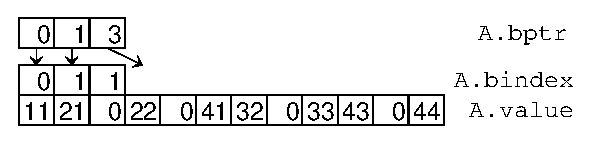
\includegraphics{storage08.eps} 
\end{flushleft}
\end{minipage}
\caption{The data structure of the BSC format (for serial and OpenMP versions).}\label{fig:storage08}}
\end{figure}
\begin{itembox}[l]{for serial and OpenMP versions}
\small
\begin{verbatim}
 1: int           n,bnr,bnc,nr,nc,bnnz;
 2: int           *bptr,*bindex;
 3: LIS_SCALAR    *value;
 4: LIS_MATRIX    A;
 5: n = 4; bnr = 2; bnc = 2; bnnz = 3; nr = (n-1)/bnr+1; nc = (n-1)/bnc+1;
 6: bptr   = (int *)malloc( (nc+1)*sizeof(int) );
 7: bindex = (int *)malloc( bnnz*sizeof(int) );
 8: value  = (LIS_SCALAR *)malloc( bnr*bnc*bnnz*sizeof(LIS_SCALAR) );
 9: lis_matrix_create(0,&A);
10: lis_matrix_set_size(A,0,n);
11:
12: bptr[0] = 0; bptr[1] = 1; bptr[2] = 3;
13: bindex[0] =  0; bindex[1] =  1; bindex[2] =  1;
14: value[0]  = 11; value[1] = 21; value[2] =  0; value[3] = 22;
15: value[4]  =  0; value[5] = 41; value[6] = 32; value[7] =  0;
16: value[8]  = 33; value[9] = 43; value[10]=  0; value[11]= 44;
17:
18:  lis_matrix_set_bsc(bnr,bnc,bnnz,bptr,bindex,value,A);
19:  lis_matrix_assemble(A);
\end{verbatim}
\end{itembox}
\newpage
\subsubsection{Creating Matrices (for MPI Version)}
Figure \ref{fig:storage08_mpi} shows how the matrix $A$ in Figure
\ref{fig:storage08} is stored in the BSC format on two processing
elements. A program to create the matrix in the BSC format on two processing elements is as follows:
\begin{figure}[h]
{\centering 
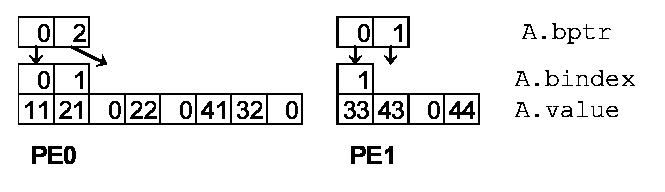
\includegraphics{storage08_mpi.eps} 
\caption{The data structure of the BSC format (for MPI version).}\label{fig:storage08_mpi}}
\end{figure}
\begin{itembox}[l]{for MPI version}
\small
\begin{verbatim}
 1: int           n,bnr,bnc,nr,nc,bnnz,my_rank;
 2: int           *bptr,*bindex;
 3: LIS_SCALAR    *value;
 4: LIS_MATRIX    A;
 5: MPI_Comm_rank(MPI_COMM_WORLD,&my_rank);
 6: if( my_rank==0 ) {n = 2; bnr = 2; bnc = 2; bnnz = 2; nr = (n-1)/bnr+1; nc = (n-1)/bnc+1;}
 7: else             {n = 2; bnr = 2; bnc = 2; bnnz = 1; nr = (n-1)/bnr+1; nc = (n-1)/bnc+1;}
 8: bptr   = (int *)malloc( (nr+1)*sizeof(int) );
 9: bindex = (int *)malloc( bnnz*sizeof(int) );
10: value  = (LIS_SCALAR *)malloc( bnr*bnc*bnnz*sizeof(LIS_SCALAR) );
11: lis_matrix_create(MPI_COMM_WORLD,&A);
12: lis_matrix_set_size(A,n,0);
13: if( my_rank==0 ) {
14:     bptr[0] = 0; bptr[1] = 2;
15:     bindex[0] =  0; bindex[1] =  1;
16:     value[0]  = 11; value[1]  = 21; value[2] =  0; value[3] = 22;
17:     value[4]  =  0; value[5]  = 41; value[6] = 32; value[7] =  0;}
18: else {
19:     bptr[0] = 0; bptr[1] = 1;
20:     bindex[0] =  1;
21:     value[0]  = 33; value[1]  = 43; value[2] =  0; value[3] = 44;}
22:  lis_matrix_set_bsc(bnr,bnc,bnnz,bptr,bindex,value,A);
23:  lis_matrix_assemble(A);
\end{verbatim}
\end{itembox}
\subsubsection{Associating Arrays}
To associate the arrays required by the BSC format with the matrix $A$, the following functions are used:
\begin{itemize}
\item \verb|C       int lis_matrix_set_bsc(int bnr, int bnc, int bnnz, int bptr[],|\\
      \verb| int bindex[], LIS_SCALAR value[], LIS_MATRIX A)|
\item \verb|Fortran subroutine lis_matrix_set_bsc(integer bnr, integer bnc, integer bnnz,|\\
      \verb| integer bptr(), integer bindex(), LIS_SCALAR value(), LIS_MATRIX A, integer ierr)|
\end{itemize}

%%%%%%%%%%%%%%%%%%%%%%%%%%%%%%%%%%%%%%%%%%%%%%%%%%%%%%%%%%%%%%%%%%
% Variable Block Row (VBR)
%%%%%%%%%%%%%%%%%%%%%%%%%%%%%%%%%%%%%%%%%%%%%%%%%%%%%%%%%%%%%%%%%%
\newpage
\subsection{Variable Block Row (VBR)}
VBR is the generalized version of BSR. The division points of the rows and columns are given by the arrays {\ttfamily row} and {\ttfamily col}. 
VBR stores the nonzero blocks (the blocks in which at least one nonzero block exists) in the same step as that for the CRS format. 
Assume that $nr$ and $nc$ are the numbers of row and column divisions, respectively, 
and that $nnzb$ denotes the number of the nonzero blocks of A, 
and $nnz$ denotes the total number of the elements of the nonzero blocks. 
VBR uses six arrays {\ttfamily bptr}, {\ttfamily bindex}, {\ttfamily
row}, {\ttfamily col}, {\ttfamily ptr} and {\ttfamily value} to store matrices.
\begin{itemize}
\item {\ttfamily row} is an integer array with a length of $nr+1$, which
      stores the starting row number of the block rows.
\item {\ttfamily col} is an integer array with a length of $nc+1$, which
      stores the starting column number of the block columns.
\item {\ttfamily bindex} is an integer array with a length of $nnzb$,
      which stores the block column numbers of the nonzero blocks.
\item {\ttfamily bptr} is an integer array with a length of $nr+1$,
      which stores the starting points of the block rows in the array {\ttfamily bindex}.
\item {\ttfamily value} is a double precision array with a length of
      $nnz$, which stores all the elements of the nonzero blocks.
\item {\ttfamily ptr} is an integer array with a length of $nnzb+1$,
      which stores the starting points of the nonzero blocks in the
      array {\ttfamily value}.
\end{itemize}
\subsubsection{Creating Matrices (for Serial and OpenMP Versions)}
The right diagram in Figure \ref{fig:storage09} shows how the matrix $A$ in Figure \ref{fig:storage09} is stored in the VBR format. A program to create the matrix in the VBR format is as follows:
\begin{figure}[h]
{\centering 
\begin{minipage}{0.3\textwidth}
\begin{flushright}
$ 
A = \left(
\begin{array}{c|cc|c}
11 &    &    &    \\ \hline
21 & 22 &    &    \\
   & 32 & 33 &    \\ \hline
41 &    & 43 & 44 \\
\end{array}\right)
$
\end{flushright}
\end{minipage}
\begin{minipage}{0.6\textwidth}
\begin{flushleft}
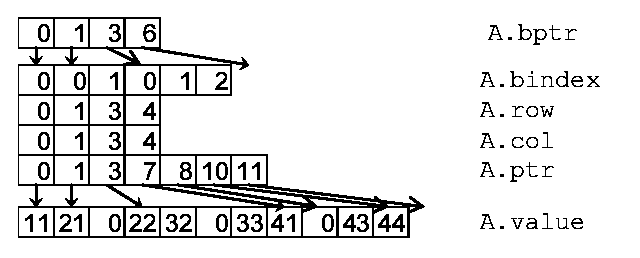
\includegraphics{storage09.eps} 
\end{flushleft}
\end{minipage}
\caption{The data structure of the VBR format (for serial and OpenMP versions).}\label{fig:storage09}}
\end{figure}
\begin{itembox}[l]{for serial and OpenMP versions}
\small
\begin{verbatim}
 1: int           n,nnz,nr,nc,bnnz;
 2: int           *row,*col,*ptr,*bptr,*bindex;
 3: LIS_SCALAR    *value;
 4: LIS_MATRIX    A;
 5: n = 4; nnz = 11; bnnz = 6; nr = 3; nc = 3;
 6: bptr   = (int *)malloc( (nr+1)*sizeof(int) );
 7: row    = (int *)malloc( (nr+1)*sizeof(int) );
 8: col    = (int *)malloc( (nc+1)*sizeof(int) );
 9: ptr    = (int *)malloc( (bnnz+1)*sizeof(int) );
10: bindex = (int *)malloc( bnnz*sizeof(int) );
11: value  = (LIS_SCALAR *)malloc( nnz*sizeof(LIS_SCALAR) );
12: lis_matrix_create(0,&A);
13: lis_matrix_set_size(A,0,n);
14:
15: bptr[0] = 0; bptr[1] = 1; bptr[2] = 3; bptr[3] = 6;
16: row[0]  = 0; row[1]  = 1; row[2]  = 3; row[3] = 4;
17: col[0]  = 0; col[1]  = 1; col[2]  = 3; col[3] = 4;
18: bindex[0] =  0; bindex[1] =  0; bindex[2] =  1; bindex[3] =  0;
19: bindex[4] =  1; bindex[5] =  2;
20: ptr[0]    =  0; ptr[1]    =  1; ptr[2]    =  3; ptr[3]    =  7;
21: ptr[4]    =  8; ptr[5]    = 10; ptr[6]    = 11;
22: value[0]  = 11; value[1]  = 21; value[2]  =  0; value[3]  = 22;
23: value[4]  = 32; value[5]  =  0; value[6]  = 33; value[7]  = 41;
24: value[8]  =  0; value[9]  = 43; value[10] = 44;
25:
26:  lis_matrix_set_vbr(nnz,nr,nc,bnnz,row,col,ptr,bptr,bindex,value,A);
27:  lis_matrix_assemble(A);
\end{verbatim}
\end{itembox}
\subsubsection{Creating Matrices (for MPI Version)}
Figure \ref{fig:storage09_mpi} shows how the matrix $A$ in Figure \ref{fig:storage09} is stored in the VBR format on two processing elements. A program to create the matrix in the VBR format on two processing elements is as follows:
\begin{figure}[h]
{\centering 
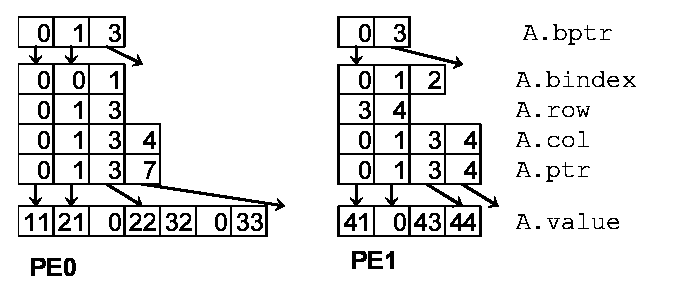
\includegraphics{storage09_mpi.eps} 
\caption{The data structure of the VBR format (for MPI version).}\label{fig:storage09_mpi}}
\end{figure}
\begin{itembox}[l]{for MPI version}
\small
\begin{verbatim}
 1: int           n,nnz,nr,nc,bnnz,my_rank;
 2: int           *row,*col,*ptr,*bptr,*bindex;
 3: LIS_SCALAR    *value;
 4: LIS_MATRIX    A;
 5: MPI_Comm_rank(MPI_COMM_WORLD,&my_rank);
 6: if( my_rank==0 ) {n = 2; nnz = 7; bnnz = 3; nr = 2; nc = 3;}
 7: else             {n = 2; nnz = 4; bnnz = 3; nr = 1; nc = 3;}
 8: bptr   = (int *)malloc( (nr+1)*sizeof(int) );
 9: row    = (int *)malloc( (nr+1)*sizeof(int) );
10: col    = (int *)malloc( (nc+1)*sizeof(int) );
11: ptr    = (int *)malloc( (bnnz+1)*sizeof(int) );
12: bindex = (int *)malloc( bnnz*sizeof(int) );
13: value  = (LIS_SCALAR *)malloc( nnz*sizeof(LIS_SCALAR) );
14: lis_matrix_create(MPI_COMM_WORLD,&A);
15: lis_matrix_set_size(A,n,0);
16: if( my_rank==0 ) {
17:     bptr[0] = 0; bptr[1] = 1; bptr[2] = 3;
18:     row[0]  = 0; row[1]  = 1; row[2]  = 3;
19:     col[0]  = 0; col[1]  = 1; col[2]  = 3; col[3] = 4;
20:     bindex[0] =  0; bindex[1] =  0; bindex[2] =  1;
21:     ptr[0]    =  0; ptr[1]    =  1; ptr[2]    =  3; ptr[3]    =  7;
22:     value[0]  = 11; value[1] = 21; value[2] =  0; value[3] = 22;
23:     value[4]  = 32; value[5] =  0; value[6] = 33;}
24: else {
25:     bptr[0] = 0; bptr[1] = 3;
26:     row[0]  = 3; row[1]  = 4;
27:     col[0]  = 0; col[1]  = 1; col[2]  = 3; col[3] = 4;
28:     bindex[0] =  0; bindex[1] =  1; bindex[2] =  2;
29:     ptr[0]    =  0; ptr[1]    =  1; ptr[2]    =  3; ptr[3]    =  4;
30:     value[0]  = 41; value[1]  =  0; value[2]  = 43; value[3]  = 44;}
31:  lis_matrix_set_vbr(nnz,nr,nc,bnnz,row,col,ptr,bptr,bindex,value,A);
32:  lis_matrix_assemble(A);
\end{verbatim}
\end{itembox}
\subsubsection{Associating Arrays}
To associate the arrays required by the VBR format with the matrix $A$, the following functions are used:
\begin{itemize}
\item \verb|C       int lis_matrix_set_vbr(int nnz, int nr, int nc, int bnnz, int row[],|\\
      \verb| int col[], int ptr[], int bptr[], int bindex[], LIS_SCALAR value[], LIS_MATRIX A)|
\item \verb|Fortran subroutine lis_matrix_set_vbr(integer nnz, integer nr, integer nc,|\\
      \verb| integer bnnz, integer row(), integer col(), integer ptr(), integer bptr(),|\\
      \verb| integer bindex(), LIS_SCALAR value(), LIS_MATRIX A, integer ierr) |
\end{itemize}

%%%%%%%%%%%%%%%%%%%%%%%%%%%%%%%%%%%%%%%%%%%%%%%%%%%%%%%%%%%%%%%%%%
% Coordinate (COO)
%%%%%%%%%%%%%%%%%%%%%%%%%%%%%%%%%%%%%%%%%%%%%%%%%%%%%%%%%%%%%%%%%%
\newpage
\subsection{Coordinate (COO)}
COO uses three arrays {\ttfamily row}, {\ttfamily col} and {\ttfamily value} to store data.
\begin{itemize}
\item {\ttfamily value} is a double precision array with a length of
      $nnz$, which stores the nonzero elements.
\item {\ttfamily row} is an integer array with a length of $nnz$, which stores the row numbers of the nonzero elements.
\item {\ttfamily col} is an integer array with a length of $nnz$, which stores the column numbers of the nonzero elements.
\end{itemize}

\subsubsection{Creating Matrices (for Serial and OpenMP Versions)}
The right diagram in Figure \ref{fig:storage10} shows how the matrix $A$ in Figure \ref{fig:storage10} is stored in the COO format. A program to create the matrix in the COO format is as follows:
\begin{figure}[h]
{\centering 
\begin{minipage}{0.3\textwidth}
\begin{flushright}
$ 
A = \left(
\begin{array}{cccc}
11 &    &    &    \\
21 & 22 &    &    \\
   & 32 & 33 &    \\
41 &    & 43 & 44 \\
\end{array}\right)
$
\end{flushright}
\end{minipage}
\begin{minipage}{0.6\textwidth}
\begin{flushleft}
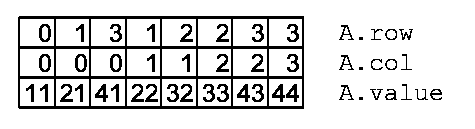
\includegraphics{storage10.eps} 
\end{flushleft}
\end{minipage}
\caption{The data structure of the COO format (for serial and OpenMP versions).}\label{fig:storage10}}
\end{figure}
\begin{itembox}[l]{for serial and OpenMP versions}
\small
\begin{verbatim}
 1: int           n,nnz;
 2: int           *row,*col;
 3: LIS_SCALAR    *value;
 4: LIS_MATRIX    A;
 5: n = 4; nnz = 8;
 6: row   = (int *)malloc( nnz*sizeof(int) );
 7: col   = (int *)malloc( nnz*sizeof(int) );
 8: value = (LIS_SCALAR *)malloc( nnz*sizeof(LIS_SCALAR) );
 9: lis_matrix_create(0,&A);
10: lis_matrix_set_size(A,0,n);
11:
12: row[0] = 0; row[1] = 1; row[2] = 3; row[3] = 1;
13: row[4] = 2; row[5] = 2; row[6] = 3; row[7] = 3;
14: col[0] = 0; col[1] = 0; col[2] = 0; col[3] = 1;
15: col[4] = 1; col[5] = 2; col[6] = 2; col[7] = 3;
16: value[0] = 11; value[1] = 21; value[2] = 41; value[3] = 22;
17: value[4] = 32; value[5] = 33; value[6] = 43; value[7] = 44;
18:
19:  lis_matrix_set_coo(nnz,row,col,value,A);
20:  lis_matrix_assemble(A);
\end{verbatim}
\end{itembox}
\newpage
\subsubsection{Creating Matrices (for MPI Version)}
Figure \ref{fig:storage10_mpi} shows how the matrix $A$ in Figure
\ref{fig:storage10} is stored in the COO format on two processing
elements. A program to create the matrix in the COO format on two processing elements is as follows:
\begin{figure}[h]
{\centering 
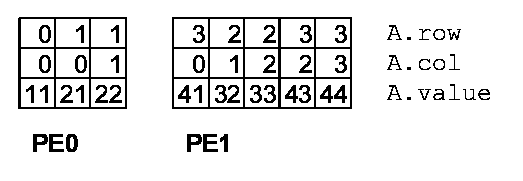
\includegraphics{storage10_mpi.eps} 
\caption{The data structure of the COO format (for MPI version).}\label{fig:storage10_mpi}}
\end{figure}
\begin{itembox}[l]{for MPI version}
\small
\begin{verbatim}
 1: int           n,nnz,my_rank;
 2: int           *row,*col;
 3: LIS_SCALAR    *value;
 4: LIS_MATRIX    A;
 5: MPI_Comm_rank(MPI_COMM_WORLD,&my_rank);
 6: if( my_rank==0 ) {n = 2; nnz = 3;}
 7: else             {n = 2; nnz = 5;}
 8: row   = (int *)malloc( nnz*sizeof(int) );
 9: col   = (int *)malloc( nnz*sizeof(int) );
10: value = (LIS_SCALAR *)malloc( nnz*sizeof(LIS_SCALAR) );
11: lis_matrix_create(MPI_COMM_WORLD,&A);
12: lis_matrix_set_size(A,n,0);
13: if( my_rank==0 ) {
14:     row[0] = 0; row[1] = 1; row[2] = 1;
15:     col[0] = 0; col[1] = 0; col[2] = 1;
16:     value[0] = 11; value[1] = 21; value[2] = 22;}
17: else {
18:     row[0] = 3; row[1] = 2; row[2] = 2; row[3] = 3; row[4] = 3;
19:     col[0] = 0; col[1] = 1; col[2] = 2; col[3] = 2; col[4] = 3;
20:     value[0] = 41; value[1] = 32; value[2] = 33; value[3] = 43; value[4] = 44;}
21:  lis_matrix_set_coo(nnz,row,col,value,A);
22:  lis_matrix_assemble(A);
\end{verbatim}
\end{itembox}
\subsubsection{Associating Arrays}
To associate the arrays required by the COO format with the matrix $A$, the following functions are used:
\begin{itemize}
\item \verb|C       int lis_matrix_set_coo(int nnz, int row[], int col[], LIS_SCALAR value[],|\\
      \verb| LIS_MATRIX A)|
\item \verb|Fortran subroutine lis_matrix_set_coo(integer nnz, integer row(), integer col(),|\\
      \verb| LIS_SCALAR value(), LIS_MATRIX A, integer ierr)|
\end{itemize}

%%%%%%%%%%%%%%%%%%%%%%%%%%%%%%%%%%%%%%%%%%%%%%%%%%%%%%%%%%%%%%%%%%
% Dense (DNS)
%%%%%%%%%%%%%%%%%%%%%%%%%%%%%%%%%%%%%%%%%%%%%%%%%%%%%%%%%%%%%%%%%%
\newpage
\subsection{Dense (DNS)}
DNS uses one array {\ttfamily value} to store data.
\begin{itemize}
\item {\ttfamily value} is a double precision array with a length of $n
      \times n$, which stores the elements with priority given to the columns.
\end{itemize}

\subsubsection{Creating Matrices (for Serial and OpenMP Versions)}
The right diagram in Figure \ref{fig:storage11} shows how the matrix $A$ in Figure \ref{fig:storage11} is stored in the DNS format. A program to create the matrix in the DNS format is as follows:
\begin{figure}[h]
{\centering 
\begin{minipage}{0.3\textwidth}
\begin{flushright}
$ 
A = \left(
\begin{array}{cccc}
11 &    &    &    \\
21 & 22 &    &    \\
   & 32 & 33 &    \\
41 &    & 43 & 44 \\
\end{array}\right)
$
\end{flushright}
\end{minipage}
\begin{minipage}{0.6\textwidth}
\begin{flushleft}

\includegraphics{storage11.eps} 
\end{flushleft}
\end{minipage}
\caption{The data structure of the DNS format (for serial and OpenMP versions).}\label{fig:storage11}}
\end{figure}
\begin{itembox}[l]{for serial and OpenMP versions}
\small
\begin{verbatim}
 1: int           n;
 2: LIS_SCALAR    *value;
 3: LIS_MATRIX    A;
 4: n = 4;
 5: value = (LIS_SCALAR *)malloc( n*n*sizeof(LIS_SCALAR) );
 6: lis_matrix_create(0,&A);
 7: lis_matrix_set_size(A,0,n);
 8:
 9: value[0] = 11; value[1] = 21; value[2] =  0; value[3] = 41;
10: value[4] =  0; value[5] = 22; value[6] = 32; value[7] =  0;
11: value[8] =  0; value[9] =  0; value[10]= 33; value[11]= 43;
12: value[12]=  0; value[13]=  0; value[14]=  0; value[15]= 44;
13:
14:  lis_matrix_set_dns(value,A);
15:  lis_matrix_assemble(A);
\end{verbatim}
\end{itembox}
\newpage
\subsubsection{Creating Matrices (for MPI Version)}
Figure \ref{fig:storage11_mpi} shows how the matrix $A$ in Figure
\ref{fig:storage11} is stored in the DNS format on two
processing elements. A program to create the matrix in the DNS format on
two processing elements is as follows:
\begin{figure}[h]
{\centering 
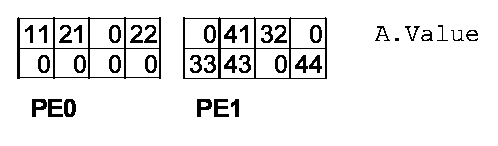
\includegraphics{storage11_mpi.eps} 
\caption{The data structure of the DNS format (for MPI version).}\label{fig:storage11_mpi}}
\end{figure}
\begin{itembox}[l]{for MPI version}
\small
\begin{verbatim}
 1: int           n,my_rank;
 2: LIS_SCALAR    *value;
 3: LIS_MATRIX    A;
 4: MPI_Comm_rank(MPI_COMM_WORLD,&my_rank);
 5: if( my_rank==0 ) {n = 2;}
 6: else             {n = 2;}
 7: value = (LIS_SCALAR *)malloc( n*n*sizeof(LIS_SCALAR) );
 8: lis_matrix_create(MPI_COMM_WORLD,&A);
 9: lis_matrix_set_size(A,n,0);
10: if( my_rank==0 ) {
11:     value[0] = 11; value[1] = 21; value[2] =  0; value[3] = 22;
12:     value[4] =  0; value[5] =  0; value[6] =  0; value[7] =  0;}
13: else {
14:     value[0] =  0; value[1] = 41; value[2] = 32; value[3] =  0;
15:     value[4] = 33; value[5] = 43; value[6] =  0; value[7] = 44;}
16:  lis_matrix_set_dns(value,A);
17:  lis_matrix_assemble(A);
\end{verbatim}
\end{itembox}
\subsubsection{Associating Arrays}
To associate the arrays required by the DNS format with the matrix $A$, the following functions are used:
\begin{itemize}
\item \verb|C       int lis_matrix_set_dns(LIS_SCALAR value[], LIS_MATRIX A)|
\item \verb|Fortran subroutine lis_matrix_set_dns(LIS_SCALAR value(), LIS_MATRIX A, integer ierr)|
\end{itemize}

%%%%%%%%%%%%%%%%%%%%%%%%%%%%%%%%%%%%%%%%%%%%%%%%%%%%%%%%%%%%%%
%%%%%%%%%%%%%%%%%%%%%%%%%%%%%%%%%%%%%%%%%%%%%%%%%%%%%%%%%%%%%%
%%%%%%%%%%%%%%%%%%%%%%%%%%%%%%%%%%%%%%%%%%%%%%%%%%%%%%%%%%%%%%
\newpage
\section{Functions}\label{sec:func}
This section describes the functions which can be employed by users.
The return values of the functions in C and the values of {\tt ierr} in Fortran are as 
follows: 
\\ \\ \\
{\bf Return Values}
\begin{namelist}{XXXXXXXXXXXXXXXXXXXX}
\item[\tt LIS\_SUCCESS(0)] ~~~~~Normal termination
\item[\tt LIS\_ILL\_OPTION(1)] ~~~~~Illegal option
\item[\tt LIS\_BREAKDOWN(2)] ~~~~~Breakdown
\item[\tt LIS\_OUT\_OF\_MEMORY(3)] ~~~~~Insufficient working memory
\item[\tt LIS\_MAXITER(4)] ~~~~~Did not converge within the maximum number of iterations
\item[\tt LIS\_NOT\_IMPLEMENTED(5)] ~~~~~Not implemented
\item[\tt LIS\_ERR\_FILE\_IO(6)] ~~~~~File I/O error
\end{namelist}

%%%%%%%%%%%%%%%%%%%%%%%%%%%%%%%%%%%%%%%%%%%%%%%%%%%%%%%%%%%%%%
\subsection{Operating Vector Elements}
Assume that the size of the vector $v$ is $global\_n$ and that the size
of the partial vectors stored on $nprocs$ processing elements 
is $local\_n$. $global\_n$ and $local\_n$ 
are called the global size and the local size, respectively.
%%%%%%%%%%%%%%%%%%%%%%%%%%%%%%%%%%%%%%%%%%%%%%%%%%%%%%%%%%%%%%
\subsubsection{lis\_vector\_create}
\begin{screen}
\verb|C       int lis_vector_create(LIS_Comm comm, LIS_VECTOR *v)|\\
\verb|Fortran subroutine lis_vector_create(LIS_Comm comm, LIS_VECTOR v, integer ierr)| 
\end{screen}
{\bf Description}\\
\indent
Create vector $v$ 
\\ \\
\noindent
{\bf Input}
\begin{namelist}{XXXXXXXXXXXXXXXXXXXX}
\item[\tt LIS\_Comm] MPI communicator
\end{namelist}
{\bf Output}
\begin{namelist}{XXXXXXXXXXXXXXXXXXXX}
\item[\tt v] Vector
\item[\tt ierr] Return code
\end{namelist}
{\bf Note}\\
\indent
For the serial and OpenMP versions, the value for {\tt comm} is ignored.
%%%%%%%%%%%%%%%%%%%%%%%%%%%%%%%%%%%%%%%%%%%%%%%%%%%%%%%%%%%%%%
\newpage
  \subsubsection{lis\_vector\_destroy}
\begin{screen}
\verb|C       int lis_vector_destroy(LIS_VECTOR v)|\\
\verb|Fortran subroutine lis_vector_destroy(LIS_VECTOR v, integer ierr)|
\end{screen}
{\bf Description}\\
\indent
Destroy vector $v$ 
\\ \\
\noindent
{\bf Input}
\begin{namelist}{XXXXXXXXXXXXXXXXXXXX}
\item[\tt v] Vector to be destroyed
\end{namelist}
{\bf Output}
\begin{namelist}{XXXXXXXXXXXXXXXXXXXX}
\item[\tt ierr] Return code
\end{namelist}
%%%%%%%%%%%%%%%%%%%%%%%%%%%%%%%%%%%%%%%%%%%%%%%%%%%%%%%%%%%%%%
  \subsubsection{lis\_vector\_duplicate}
\begin{screen}
\verb|C       int lis_vector_duplicate(void *vin, LIS_VECTOR *vout)|
\verb|Fortran subroutine lis_vector_duplicate(LIS_VECTOR vin, LIS_VECTOR vout,|\\
\verb|         integer ierr)|
\end{screen}
{\bf Description}\\
\indent
Create vector $v_{out}$ which has the same information as $v_{in}$
\\ \\
\noindent
{\bf Input}
\begin{namelist}{XXXXXXXXXXXXXXXXXXXX}
\item[\tt vin] Source vector
\end{namelist}
{\bf Output}
\begin{namelist}{XXXXXXXXXXXXXXXXXXXX}
\item[\tt vout] Destination vector
\item[\tt ierr] Return code
\end{namelist}
{\bf Note}\\
\indent
The function \verb|lis_vector_duplicate| does not copy the values, 
but only reserves an area. To copy the values as well, 
the function \verb|lis_vector_copy| must be used after this function.
%%%%%%%%%%%%%%%%%%%%%%%%%%%%%%%%%%%%%%%%%%%%%%%%%%%%%%%%%%%%%%
\newpage
\subsubsection{lis\_vector\_set\_size}
\begin{screen}
\verb|C       int lis_vector_set_size(LIS_VECTOR v, int local_n, int global_n)|\\
\verb|Fortran subroutine lis_vector_set_size(LIS_VECTOR v, integer local_n,|\\
\verb|         integer global_n, integer ierr)| 
\end{screen}
{\bf Description}\\
\indent
Assign size of vector $v$ 
\\ \\
\noindent
{\bf Input}
\begin{namelist}{XXXXXXXXXXXXXXXXXXXX}
\item[\tt v] Vector
\item[\tt local\_n] Size of partial vector
\item[\tt global\_n] Size of global vector
\end{namelist}
{\bf Output}
\begin{namelist}{XXXXXXXXXXXXXXXXXXXX}
\item[\tt ierr] Return code
\end{namelist}
{\bf Note}\\
\indent
Either $local\_n$ or $global\_n$ must be provided. 
This function can create a vector in one of the following ways: 
Creates partial vectors of size $local\_n$ if $local\_n$ is 
given, or creates partial vectors stored on a given number of
processing elements, if $global\_n$ is given.

In the case of the serial and OpenMP versions, $local\_n$ $=$ $global\_n$. 
It means that both \\
\verb|lis_vector_set_size(v,n,0)| and \verb|lis_vector_set_size(v,0,n)| 
create a vector of size $n$. 
%%%%%%%%%%%%%%%%%%%%%%%%%%%%%%%%%%%%%%%%%%%%%%%%%%%%%%%%%%%%%%
  \subsubsection{lis\_vector\_get\_size}
\begin{screen}
\verb|C       int lis_vector_get_size(LIS_VECTOR v, int *local_n, int *global_n)|
\verb|Fortran subroutine lis_vector_get_size(LIS_VECTOR v, integer local_n,|\\
\verb|         integer global_n, integer ierr)|
\end{screen}
{\bf Description}\\
\indent
Get size of vector $v$
\\ \\
\noindent
{\bf Input}
\begin{namelist}{XXXXXXXXXXXXXXXXXXXX}
\item[\tt v] Vector
\end{namelist}
{\bf Output}
\begin{namelist}{XXXXXXXXXXXXXXXXXXXX}
\item[\tt local\_n] Size of partial vector
\item[\tt global\_n] Size of global vector
\item[\tt ierr] Return code
\end{namelist}
{\bf Note}\\
\indent
In the case of the serial and OpenMP versions, $local\_n$ $=$ $global\_n$. 
%%%%%%%%%%%%%%%%%%%%%%%%%%%%%%%%%%%%%%%%%%%%%%%%%%%%%%%%%%%%%%
  \subsubsection{lis\_vector\_get\_range}
\begin{screen}
\verb|C       int lis_vector_get_range(LIS_VECTOR v, int *is, int *ie)|
\verb|Fortran subroutine lis_vector_get_range(LIS_VECTOR v, integer is, integer ie,|\\
\verb|         integer ierr) |
\end{screen}
{\bf Description}\\
\indent
Get location of partial vector $v$ in global vector 
\\ \\
\noindent
{\bf Input}
\begin{namelist}{XXXXXXXXXXXXXXXXXXXX}
\item[\tt v] Partial vector
\end{namelist}
{\bf Output}
\begin{namelist}{XXXXXXXXXXXXXXXXXXXX}
\item[\tt is] Location where partial vector $v$ starts in global vector
\item[\tt ie] $1 +$ location where partial vector $v$ ends in
	  global vector
\item[\tt ierr] Return code
\end{namelist}
{\bf Note}\\
\indent
For the serial and OpenMP versions, a vector of size $n$ results in $is = 0$ and $ie = n$. 
%%%%%%%%%%%%%%%%%%%%%%%%%%%%%%%%%%%%%%%%%%%%%%%%%%%%%%%%%%%%%%
  \subsubsection{lis\_vector\_set\_value}
\begin{screen}
\verb|C       int lis_vector_set_value(int flag, int i, LIS_SCALAR value, LIS_VECTOR v)|
\verb|Fortran subroutine lis_vector_set_value(integer flag, integer i, LIS_SCALAR value,|\\
\verb|         LIS_VECTOR v, integer ierr)|
\end{screen}
{\bf Description}\\
\indent
Assign scalar $value$ to $i$-th row of vector $v$
\\ \\
\noindent
{\bf Input}
\begin{namelist}{XXXXXXXXXXXXXXXXXXXX}
\item[\tt flag] \begin{description}
\item[\tt LIS\_INS\_VALUE]: {\tt v[$i$] = $value$}
\item[\tt LIS\_ADD\_VALUE]: {\tt v[$i$] = v[$i$] + $value$}
\end{description}
\item[\tt i] Location where value is assigned
\item[\tt value] Scalar value to be assigned
\item[\tt v] Destination vector
\end{namelist}
{\bf Output}
\begin{namelist}{XXXXXXXXXXXXXXXXXXXX}
\item[\tt v] Vector with scalar $value$ assigned to $i$-th row
\item[\tt ierr] Return code
\end{namelist}
{\bf Note}\\
\indent
For the MPI version, the $i$-th row of the global vector must be specified instead 
of the $i$-th row of the partial vector.
%%%%%%%%%%%%%%%%%%%%%%%%%%%%%%%%%%%%%%%%%%%%%%%%%%%%%%%%%%%%%%
  \subsubsection{lis\_vector\_get\_value}
\begin{screen}
\verb|C       int lis_vector_get_value(LIS_VECTOR v, int i, LIS_SCALAR *value)|
\verb|Fortran subroutine lis_vector_get_value(LIS_VECTOR v, integer i, LIS_SCALAR value,|\\
\verb|         integer ierr)|
\end{screen}
{\bf Description}\\
\indent
Get value of $i$-th row of vector $v$
\\ \\
\noindent
{\bf Input}
\begin{namelist}{XXXXXXXXXXXXXXXXXXXX}
\item[\tt i] Location where value should be assigned
\item[\tt v] Destination vector
\end{namelist}
{\bf Output}
\begin{namelist}{XXXXXXXXXXXXXXXXXXXX}
\item[\tt value] Value of $i$-th row
\item[\tt ierr] Return code
\end{namelist}
{\bf Note}\\
\indent
For the MPI version, the $i$-th row of the global vector must be
specified instead of  
the $i$-th row of the partial vector.
%%%%%%%%%%%%%%%%%%%%%%%%%%%%%%%%%%%%%%%%%%%%%%%%%%%%%%%%%%%%%%
  \subsubsection{lis\_vector\_set\_values}
\begin{screen}
\verb|C       int lis_vector_set_values(int flag, int count, int index[],|\\
\verb|         LIS_SCALAR value[], LIS_VECTOR v)|\\
\verb|Fortran subroutine lis_vector_set_values(integer flag, integer count,|\\
\verb|         integer index(), LIS_SCALAR value(), LIS_VECTOR v, integer ierr)|
\end{screen}
{\bf Description}\\
\indent
Assign scalar values {\tt value[$i$]} to the {\tt index[$i$]}-th row of vector $v$
\\ \\
\noindent
{\bf Input}
\begin{namelist}{XXXXXXXXXXXXXXXXXXXX}
\item[\tt flag] \begin{description}
\item[\tt LIS\_INS\_VALUE]: {\tt v[index[$i$]] = value[$i$]}
\item[\tt LIS\_ADD\_VALUE]: {\tt v[index[$i$]] = v[index[$i$]] + value[$i$]}
\end{description}
\item[\tt count] Number of elements of array which stores scalar values to be assigned
\item[\tt index] Array which stores location where scalar values should be assigned
\item[\tt value] Array which stores scalar values to be assigned
\item[\tt v] Destination vector
\end{namelist}
{\bf Output}
\begin{namelist}{XXXXXXXXXXXXXXXXXXXX}
\item[\tt v] Vector with scalar {\tt value[$i$]} assigned to its {\tt index[$i$]}-th row
\item[\tt ierr] Return code
\end{namelist}
{\bf Note}\\
\indent
For the MPI version, the {\tt index[$i$]}-th row of the global vector must be specified instead 
of the {\tt index[$i$]}-th row of the partial vector.
%%%%%%%%%%%%%%%%%%%%%%%%%%%%%%%%%%%%%%%%%%%%%%%%%%%%%%%%%%%%%%
  \subsubsection{lis\_vector\_get\_values}
\begin{screen}
\verb|C       int lis_vector_get_values(LIS_VECTOR v, int start, int count,|\\
\verb|         LIS_SCALAR value[])|\\
\verb|Fortran subroutine lis_vector_get_values(LIS_VECTOR v, integer start,|\\
\verb|         integer count, LIS_SCALAR value(), integer ierr)|
\end{screen}
{\bf Description}\\
\indent
Get scalar values of $start+i$-th row of vector $v$, 
where $i=0,1,...,count-1$
\\ \\
\noindent
{\bf Input}
\begin{namelist}{XXXXXXXXXXXXXXXXXXXX}
\item[\tt start] Starting location 
\item[\tt count] Number of values to get
\item[\tt v] Destination vector
\end{namelist}
{\bf Output}
\begin{namelist}{XXXXXXXXXXXXXXXXXXXX}
\item[\tt value] Vector to store scalar values
\item[\tt ierr] Return code
\end{namelist}
{\bf Note}\\
\indent
For the MPI version, the $start+i$-th row of the global vector
must be specified instead of 
the $start+i$-th row of the partial vector.
%%%%%%%%%%%%%%%%%%%%%%%%%%%%%%%%%%%%%%%%%%%%%%%%%%%%%%%%%%%%%%
\newpage
  \subsubsection{lis\_vector\_scatter}
\begin{screen}
\verb|C       int lis_vector_scatter(LIS_SCALAR value[], LIS_VECTOR v)|\\
\verb|Fortran subroutine lis_vector_scatter(LIS_SCALAR value(), LIS_VECTOR v, integer ierr)|
\end{screen}
{\bf Description}\\
\indent
Assign scalar values of $i$-th row of vector $v$, 
where $i=0,1,..., global\_n-1$
\\ \\
\noindent
{\bf Input}
\begin{namelist}{XXXXXXXXXXXXXXXXXXXX}
\item[\tt value] Array which stores scalar values to be assigned
\end{namelist}
{\bf Output}
\begin{namelist}{XXXXXXXXXXXXXXXXXXXX}
\item[\tt v] Destination vector
\item[\tt ierr] Return code
\end{namelist}
{\bf Note}\\
\indent
%%%%%%%%%%%%%%%%%%%%%%%%%%%%%%%%%%%%%%%%%%%%%%%%%%%%%%%%%%%%%%
  \subsubsection{lis\_vector\_gather}
\begin{screen}
\verb|C       int lis_vector_gather(LIS_VECTOR v, LIS_SCALAR value[])|\\
\verb|Fortran subroutine lis_vector_gather(LIS_VECTOR v, LIS_SCALAR value(), integer ierr)|
\end{screen}
{\bf Description}\\
\indent
Get scalar values of $i$-th row of vector $v$, 
where $i=0,1,..., global\_n-1$
\\ \\
\noindent
{\bf Input}
\begin{namelist}{XXXXXXXXXXXXXXXXXXXX}
\item[\tt v] Source vector
\end{namelist}
{\bf Output}
\begin{namelist}{XXXXXXXXXXXXXXXXXXXX}
\item[\tt value] Vector to store scalar values
\item[\tt ierr] Return code
\end{namelist}
{\bf Note}\\
\indent
%%%%%%%%%%%%%%%%%%%%%%%%%%%%%%%%%%%%%%%%%%%%%%%%%%%%%%%%%%%%%%
\newpage
  \subsubsection{lis\_vector\_copy}
\begin{screen}
\verb|C       int lis_vector_copy(LIS_VECTOR x, LIS_VECTOR y)|\\
\verb|Fortran subroutine lis_vector_copy(LIS_VECTOR x, LIS_VECTOR y, integer ierr)|
\end{screen}
{\bf Description}\\
\indent
Copy vector $x$
\\ \\
\noindent
{\bf Input}
\begin{namelist}{XXXXXXXXXXXXXXXXXXXX}
\item[\tt x] Source vector
\end{namelist}
{\bf Output}
\begin{namelist}{XXXXXXXXXXXXXXXXXXXX}
\item[\tt y] Destination vector
\item[\tt ierr] Return code
\end{namelist}
%%%%%%%%%%%%%%%%%%%%%%%%%%%%%%%%%%%%%%%%%%%%%%%%%%%%%%%%%%%%%%
  \subsubsection{lis\_vector\_set\_all}
\begin{screen}
\verb|C       int lis_vector_set_all(LIS_SCALAR value, LIS_VECTOR x)|
\verb|Fortran subroutine lis_vector_set_all(LIS_SCALAR value, LIS_VECTOR x, integer ierr)|
\end{screen}
{\bf Description}\\
\indent
Assign scalar $value$ to all elements of vector $v$
\\ \\
\noindent
{\bf Input}
\begin{namelist}{XXXXXXXXXXXXXXXXXXXX}
\item[\tt value] Scalar value to be assigned
\item[\tt v] Destination vector
\end{namelist}
{\bf Output}
\begin{namelist}{XXXXXXXXXXXXXXXXXXXX}
\item[\tt v] Vector with $value$ assigned to all elements
\item[\tt ierr] Return code
\end{namelist}
%%%%%%%%%%%%%%%%%%%%%%%%%%%%%%%%%%%%%%%%%%%%%%%%%%%%%%%%%%%%%%
\newpage
\subsection{Operating Matrix Elements}
Assume that the size of the matrix $A$ is $global\_n$ $\times$ $global\_n$
and that the size of each partial matrix stored on $nprocs$ 
processing elements is $local\_n$ $\times$ $global\_n$. Here, $global\_n$
and $local\_n$ are called the number of the rows of the global matrix
and the number of the rows of the partial matrix, respectively. 
  \subsubsection{lis\_matrix\_create}
\begin{screen}
\verb|C       int lis_matrix_create(LIS_Comm comm, LIS_MATRIX *A)|
\verb|Fortran subroutine lis_matrix_create(LIS_Comm comm, LIS_MATRIX A, integer ierr)|
\end{screen}
{\bf Description}\\
\indent
Create matrix $A$
\\ \\
\noindent
{\bf Input}
\begin{namelist}{XXXXXXXXXXXXXXXXXXXX}
\item[\tt LIS\_Comm] MPI communicator
\end{namelist}
{\bf Output}
\begin{namelist}{XXXXXXXXXXXXXXXXXXXX}
\item[\tt A] Matrix
\item[\tt ierr] Return code
\end{namelist}
{\bf Note}\\
\indent
For the sequential and the OpenMP versions, the value for {\tt comm} is ignored. 
%%%%%%%%%%%%%%%%%%%%%%%%%%%%%%%%%%%%%%%%%%%%%%%%%%%%%%%%%%%%%%
  \subsubsection{lis\_matrix\_destroy}
\begin{screen}
\verb|C       int lis_matrix_destroy(LIS_MATRIX A)|\\
\verb|Fortran subroutine lis_matrix_destroy(LIS_MATRIX A, integer ierr)|
\end{screen}
{\bf Description}\\
\indent
Destroy matrix $A$
\\ \\
\noindent
{\bf Input}
\begin{namelist}{XXXXXXXXXXXXXXXXXXXX}
\item[\tt A] Matrix to be destroyed
\end{namelist}
{\bf Output}
\begin{namelist}{XXXXXXXXXXXXXXXXXXXX}
\item[\tt ierr] Return code
\end{namelist}
%%%%%%%%%%%%%%%%%%%%%%%%%%%%%%%%%%%%%%%%%%%%%%%%%%%%%%%%%%%%%%
\newpage
  \subsubsection{lis\_matrix\_duplicate}
\begin{screen}
\verb|C       int lis_matrix_duplicate(LIS_MATRIX Ain, LIS_MATRIX *Aout)|
\verb|Fortran subroutine lis_matrix_duplicate(LIS_MATRIX Ain, LIS_MATRIX Aout,|\\
\verb|         integer ierr)|
\end{screen}
{\bf Description}\\
\indent
Create matrix $A_{out}$ which has the same information as the
original $A_{in}$
\\ \\
\noindent
{\bf Input}
\begin{namelist}{XXXXXXXXXXXXXXXXXXXX}
\item[\tt Ain] Source matrix
\end{namelist}
{\bf Output}
\begin{namelist}{XXXXXXXXXXXXXXXXXXXX}
\item[\tt Aout] Destination matrix
\item[\tt ierr] Return code
\end{namelist}
{\bf Note}\\
\indent
The function \verb|lis_matrix_duplicate| does not copy the values of 
the elements of the matrix, but only reserves an area. 
To copy the values of the elements as well, the function \verb|lis_matrix_copy| must be used.
%%%%%%%%%%%%%%%%%%%%%%%%%%%%%%%%%%%%%%%%%%%%%%%%%%%%%%%%%%%%%%
  \subsubsection{lis\_matrix\_malloc}
\begin{screen}
\verb|C       int lis_matrix_malloc(LIS_MATRIX A, int nnz_row, int nnz[])|
\verb|Fortran subroutine lis_matrix_malloc(LIS_MATRIX A, integer nnz_row, integer nnz[],|\\
\verb|         integer ierr)|
\end{screen}
{\bf Description}\\
\indent
Allocate memory for matrix $A$
\\ \\
\noindent
{\bf Input}
\begin{namelist}{XXXXXXXXXXXXXXXXXXXX}
\item[\tt A] Matrix
\item[\tt nnz\_row] Average number of nonzero elements
\item[\tt nnz] Array of numbers of nonzero elements in each row
\end{namelist}
{\bf Output}
\begin{namelist}{XXXXXXXXXXXXXXXXXXXX}
\item[\tt ierr] Return code
\end{namelist}
{\bf Note}\\
\indent
Either \verb|nnz_row| or \verb|nnz| must be provided.
%%%%%%%%%%%%%%%%%%%%%%%%%%%%%%%%%%%%%%%%%%%%%%%%%%%%%%%%%%%%%%
\newpage
  \subsubsection{lis\_matrix\_set\_value}
\begin{screen}
\verb|C       int lis_matrix_set_value(int flag, int i, int j, LIS_SCALAR value,|\\
\verb|         LIS_MATRIX A)|\\
\verb|Fortran subroutine lis_matrix_set_value(integer flag, integer i, integer j,|\\
\verb|         LIS_SCALAR value, LIS_MATRIX A, integer ierr)|
\end{screen}
{\bf Description}\\
\indent
Assign value to $(i, j)$ element of matrix $A$
\\ \\
\noindent
{\bf Input}
\begin{namelist}{XXXXXXXXXXXXXXXXXXXX}
\item[\tt flag] \begin{description}
\item[\tt LIS\_INS\_VALUE]: $A(i,j) = value$
\item[\tt LIS\_ADD\_VALUE]: $A(i,j) = A(i,j) + value$
\end{description}
\item[\tt i] Row number of matrix
\item[\tt j] Column number of matrix
\item[\tt value] Value to be assigned
\item[\tt A] Matrix
\end{namelist}
{\bf Output}
\begin{namelist}{XXXXXXXXXXXXXXXXXXXX}
\item[\tt A] Matrix 
\item[\tt ierr] Return code
\end{namelist}
\noindent
{\bf Note}\\
\indent
For the MPI version, the $i$-th row and the $j$-th column of the global matrix must 
be specified, instead of the $i$-th row and the $j$-th column of the partial matrix. 

The function \verb|lis_matrix_set_value| stores the assigned value in a temporary internal format. 
For this reason, when \verb|lis_matrix_set_value| is used, 
the function \verb|lis_matrix_assemble| must be called. 
%%%%%%%%%%%%%%%%%%%%%%%%%%%%%%%%%%%%%%%%%%%%%%%%%%%%%%%%%%%%%%
  \subsubsection{lis\_matrix\_assemble}
\begin{screen}
\verb|C       int lis_matrix_assemble(LIS_MATRIX A)|\\
\verb|Fortran subroutine lis_matrix_assemble(LIS_MATRIX A, integer ierr)|
\end{screen}
{\bf Description}\\
\indent
Build matrix $A$ in specified storage format
\\ \\
\noindent
{\bf Input}
\begin{namelist}{XXXXXXXXXXXXXXXXXXXX}
\item[\tt A] Matrix
\end{namelist}
{\bf Output}
\begin{namelist}{XXXXXXXXXXXXXXXXXXXX}
\item[\tt A] Matrix built in specified storage format
\item[\tt ierr] Return code
\end{namelist}
%%%%%%%%%%%%%%%%%%%%%%%%%%%%%%%%%%%%%%%%%%%%%%%%%%%%%%%%%%%%%%
  \subsubsection{lis\_matrix\_set\_size}
\begin{screen}
\verb|int lis_matrix_set_size(LIS_MATRIX A, int local_n, int global_n)|
\verb|Fortran subroutine lis_matrix_set_size(LIS_MATRIX A, integer local_n,|\\
\verb|         integer global_n, integer ierr)|
\end{screen}
{\bf Description}\\
\indent
Assign size of matrix $A$ 
\\ \\
\noindent
{\bf Input}
\begin{namelist}{XXXXXXXXXXXXXXXXXXXX}
\item[\tt A] Matrix
\item[\tt local\_n] Number of rows of partial matrix
\item[\tt global\_n] Number of rows of global matrix
\end{namelist}
{\bf Output}
\begin{namelist}{XXXXXXXXXXXXXXXXXXXX}
\item[\tt ierr] Return code
\end{namelist}
{\bf Note}\\
\indent
Either $local\_n$ or $global\_n$ must be provided. 
This function can create matrices in one of the following two ways: 
Create partial matrices of size $local\_n \times N$ if $local\_n$ is given, or 
create partial matrices of size $global\_n \times global\_n$ is stored 
in a given number of processing elements, if $global\_n$ is given. 
$N$ represents the total sum of $local\_n$. 

In case of the serial and OpenMP versions, $local\_n$ is equal to $global\_n$. 
It means that both \\
\verb|lis_matrix_set_size(A,n,0)| and \verb|lis_matrix_set_size(A,0,n)|
create a matrix of $n \times n$.

For the MPI version, \verb|lis_matrix_set_size(A,n,0)| creates on the processing element $p$ 
a partial matrix of size $n_p \times N$, where $N$ is the total sum of $n_p$. 
On the other hand, \verb|lis_matrix_set_size(A,0,n)| creates 
on the processing element $p$ a partial matrix of size $m_p \times n$, where $m_p$ is the number of 
the partial matrix, which is determined by the library.
%%%%%%%%%%%%%%%%%%%%%%%%%%%%%%%%%%%%%%%%%%%%%%%%%%%%%%%%%%%%%%
  \subsubsection{lis\_matrix\_get\_size}
\begin{screen}
\verb|C       int lis_matrix_get_size(LIS_MATRIX A, int *local_n, int *global_n)|
\verb|Fortran subroutine lis_matrix_get_size(LIS_MATRIX A, integer local_n,|\\
\verb|         integer global_n, integer ierr)|
\end{screen}
{\bf Description}\\
\indent
Get size of matrix $A$
\\ \\
\noindent
{\bf Input}
\begin{namelist}{XXXXXXXXXXXXXXXXXXXX}
\item[\tt A] Matrix
\end{namelist}
{\bf Output}
\begin{namelist}{XXXXXXXXXXXXXXXXXXXX}
\item[\tt local\_n] Number of rows of partial matrix
\item[\tt global\_n] Number of rows of global matrix
\item[\tt ierr] Return code
\end{namelist}
{\bf Note}\\
\indent
In case of the serial and OpenMP versions, $local\_n$ $=$ $global\_n$. 
%%%%%%%%%%%%%%%%%%%%%%%%%%%%%%%%%%%%%%%%%%%%%%%%%%%%%%%%%%%%%%
  \subsubsection{lis\_matrix\_get\_range}
\begin{screen}
\verb|C       int lis_matrix_get_range(LIS_MATRIX A, int *is, int *ie)|
\verb|Fortran subroutine lis_matrix_get_range(LIS_MATRIX A, integer is, integer ie,|\\
\verb|         integer ierr)|
\end{screen}
{\bf Description}\\
\indent
Get location of partial matrix $A$ in global matrix 
\\ \\
\noindent
{\bf Input}
\begin{namelist}{XXXXXXXXXXXXXXXXXXXX}
\item[\tt A] Partial matrix
\end{namelist}
{\bf Output}
\begin{namelist}{XXXXXXXXXXXXXXXXXXXX}
\item[\tt is] Location where partial matrix $A$ starts in global matrix
\item[\tt ie] $1 + $ location where partial matrix $A$ ends in
	  global matrix
\item[\tt ierr] Return code
\end{namelist}
{\bf Note}\\
\indent
For the serial and OpenMP versions, a matrix of $n \times n$ results in $is = 0$ and $ie = n$.
%%%%%%%%%%%%%%%%%%%%%%%%%%%%%%%%%%%%%%%%%%%%%%%%%%%%%%%%%%%%%%
\newpage
  \subsubsection{lis\_matrix\_set\_type}
\begin{screen}
\verb|C       int lis_matrix_set_type(LIS_MATRIX A, int matrix_type)|
\verb|Fortran subroutine lis_matrix_set_type(LIS_MATRIX A, int matrix_type, integer ierr)|
\end{screen}
{\bf Description}\\
\indent
Assign storage format
\\ \\
\noindent
{\bf Input}
\begin{namelist}{XXXXXXXXXXXXXXXXXXXX}
\item[\tt A] Matrix
\item[\tt matrix\_type] Storage format
\end{namelist}
{\bf Output}
\begin{namelist}{XXXXXXXXXXXXXXXXXXXX}
\item[\tt ierr] Return code
\end{namelist}
\noindent
{\bf Note}\\
\indent
\verb+matrix_type+ of $A$ is \verb+LIS_MATRIX_CRS+ when the matrix is created. 
The table below shows the available storage formats for \verb+matrix_type+.
\\ \\
\begin{minipage}[t]{\textwidth}
\begin{center}
\begin{tabular}{lll}\hline\hline
storage format  & & matrix\_type \\ \hline
Compressed Row Storage & (CRS) & \verb|LIS_MATRIX_CRS| \\
Compressed Column Storage & (CCS) & \verb|LIS_MATRIX_CCS| \\
Modified Compressed Sparse Row & (MSR) & \verb|LIS_MATRIX_MSR| \\
Diagonal &(DIA) & \verb|LIS_MATRIX_DIA| \\
Ellpack-Itpack generalized diagonal &(ELL) & \verb|LIS_MATRIX_ELL| \\
Jagged Diagonal &(JDS) & \verb|LIS_MATRIX_JDS| \\
Block Sparse Row & (BSR) & \verb|LIS_MATRIX_BSR| \\
Block Sparse Column &(BSC) & \verb|LIS_MATRIX_BSC| \\
Variable Block Row &(VBR) & \verb|LIS_MATRIX_VBR| \\
Dense &	(DNS) & \verb|LIS_MATRIX_DNS| \\
Coordinate & (COO) & \verb|LIS_MATRIX_COO| \\
\hline         
\end{tabular}
\end{center}
\end{minipage}
%%%%%%%%%%%%%%%%%%%%%%%%%%%%%%%%%%%%%%%%%%%%%%%%%%%%%%%%%%%%%%
  \subsubsection{lis\_matrix\_get\_type}
\begin{screen}
\verb|C       int lis_matrix_get_type(LIS_MATRIX A, int *matrix_type)|
\verb|Fortran subroutine lis_matrix_get_type(LIS_MATRIX A, integer matrix_type,|\\
\verb|         integer ierr)|
\end{screen}
{\bf Description}\\
\indent
Get storage format
\\ \\
\noindent
{\bf Input}
\begin{namelist}{XXXXXXXXXXXXXXXXXXXX}
\item[\tt A] Matrix
\end{namelist}
{\bf Output}
\begin{namelist}{XXXXXXXXXXXXXXXXXXXX}
\item[\tt matrix\_type] Storage format
\item[\tt ierr] Return code
\end{namelist}
%%%%%%%%%%%%%%%%%%%%%%%%%%%%%%%%%%%%%%%%%%%%%%%%%%%%%%%%%%%%%%
  \subsubsection{lis\_matrix\_set\_blocksize}
\begin{screen}
\verb|C       int lis_matrix_set_blocksize(LIS_MATRIX A, int bnr, int bnc, int row[],|\\
\verb|         int col[])|\\
\verb|Fortran subroutine lis_matrix_set_blocksize(LIS_MATRIX A, integer bnr, integer bnc,|\\
\verb|         integer row[], integer col[], integer ierr)|
\end{screen}
{\bf Description}\\
\indent
Assign block size for BSR, BSC, and VBR
\\ \\
\noindent
{\bf Input}
\begin{namelist}{XXXXXXXXXXXXXXXXXXXX}
\item[\tt A] Matrix
\item[\tt bnr] Row block size for BSR (BSC) or number of row blocks for VBR
\item[\tt bnc] Column block size for BSR (BSC) or number of column blocks for VBR
\item[\tt row] Array of row division information about VBR
\item[\tt col] Array of column division information about VBR
\end{namelist}
{\bf Output}
\begin{namelist}{XXXXXXXXXXXXXXXXXXXX}
\item[\tt ierr] Return code
\end{namelist}
%%%%%%%%%%%%%%%%%%%%%%%%%%%%%%%%%%%%%%%%%%%%%%%%%%%%%%%%%%%%%%
  \subsubsection{lis\_matrix\_convert}
\begin{screen}
\verb|C       int lis_matrix_convert(LIS_MATRIX Ain, LIS_MATRIX Aout)|\\
\verb|Fortran subroutine lis_matrix_convert(LIS_MATRIX Ain, LIS_MATRIX Aout, integer ierr)|
\end{screen}
{\bf Description}\\
\indent
Convert matrix $A_{in}$ into $A_{out}$ of type specified with {\tt lis\_matrix\_set\_type}
\\ \\
\noindent
{\bf Input}
\begin{namelist}{XXXXXXXXXXXXXXXXXXXX}
\item[\tt Ain] Source matrix
\end{namelist}
{\bf Output}
\begin{namelist}{XXXXXXXXXXXXXXXXXXXX}
\item[\tt Aout] Matrix converted into specified type
\item[\tt ierr] Return code
\end{namelist}
{\bf Note}\\
\indent
The specification of the converted storage format is set to \verb|Aout| by 
using \verb|lis_matrix_set_type|. 
The specification of the block size of BSR, BSC, and VBR is set to \verb|Aout| by 
using \verb|lis_matrix_set_blocksize|. 

In converting the storage type of the source matrix into a specified type, 
the conversions indicated by one in the table below are performed directly, 
and the other conversions are made via the indicated types. 
The conversions with no indication are made via the CRS type.
\\ \vspace*{5mm}

\begin{tabular}{|c|c|c|c|c|c|c|c|c|c|c|c|}
\hline
Src \textbackslash Dst & CRS & CCS & MSR & DIA & ELL & JDS & BSR & BSC & VBR & DNS & COO \\ \hline
CRS    &  1  &  1  &  1  &  1  &  1  &  1  &  1  &  CCS  &  1  &  1  &  1  \\ \hline
COO    &  1  &  1  &  1  & CRS  & CRS & CRS & CRS & CCS & CRS & CRS &  1  \\ \hline
\end{tabular}
%%%%%%%%%%%%%%%%%%%%%%%%%%%%%%%%%%%%%%%%%%%%%%%%%%%%%%%%%%%%%%
  \subsubsection{lis\_matrix\_copy}
\begin{screen}
\verb|C       int lis_matrix_copy(LIS_MATRIX Ain, LIS_MATRIX Aout)|
\verb|Fortran subroutine lis_matrix_copy(LIS_MATRIX Ain, LIS_MATRIX Aout, integer ierr) |
\end{screen}
{\bf Description}\\
\indent
Copy values of matrix elements
\\ \\
\noindent
{\bf Input}
\begin{namelist}{XXXXXXXXXXXXXXXXXXXX}
\item[\tt Ain] Source matrix
\end{namelist}
{\bf Output}
\begin{namelist}{XXXXXXXXXXXXXXXXXXXX}
\item[\tt Aout] Destination matrix
\item[\tt ierr] Return code
\end{namelist}
%%%%%%%%%%%%%%%%%%%%%%%%%%%%%%%%%%%%%%%%%%%%%%%%%%%%%%%%%%%%%%
  \subsubsection{lis\_matrix\_get\_diagonal}
\begin{screen}
\verb|C       int lis_matrix_get_diagonal(LIS_MATRIX A, LIS_VECTOR d)|\\
\verb|Fortran subroutine lis_matrix_get_diagonal(LIS_MATRIX A, LIS_VECTOR d, integer ierr) |
\end{screen}
{\bf Description}\\
\indent
Store diagonal elements of matrix $A$ to vector $d$
\\ \\
\noindent
{\bf Input}
\begin{namelist}{XXXXXXXXXXXXXXXXXXXX}
\item[\tt A] Matrix
\end{namelist}
{\bf Output}
\begin{namelist}{XXXXXXXXXXXXXXXXXXXX}
\item[\tt d] Vector which stores diagonal elements of matrix
\item[\tt ierr] Return code
\end{namelist}
%%%%%%%%%%%%%%%%%%%%%%%%%%%%%%%%%%%%%%%%%%%%%%%%%%%%%%%%%%%%%%
\newpage
  \subsubsection{lis\_matrix\_set\_crs}
\begin{screen}
\verb|C       int lis_matrix_set_crs(int nnz, int ptr[], int index[], LIS_SCALAR value[],|\\
\verb|         LIS_MATRIX A)|\\
\verb|Fortran subroutine lis_matrix_set_crs(integer nnz, integer row(), integer index(),|\\
\verb|         LIS_SCALAR value(), LIS_MATRIX A, integer ierr)|
\end{screen}
{\bf Description}\\
\indent
Set matrix $A$ in CRS format
\\ \\
\noindent
{\bf Input}
\begin{namelist}{XXXXXXXXXXXXXXXXXXXX}
\item[\tt nnz] Number of nonzero elements
\item[\tt ptr, index, value] Arrays for CRS format
\item[\tt A] Matrix
\end{namelist}
{\bf Output}
\begin{namelist}{XXXXXXXXXXXXXXXXXXXX}
\item[\tt A] Matrix and associated arrays
\end{namelist}
\noindent
{\bf Note}\\
\indent
When \verb|lis_matrix_set_crs| is used, 
the function \verb|lis_matrix_assemble| must be called. 
%%%%%%%%%%%%%%%%%%%%%%%%%%%%%%%%%%%%%%%%%%%%%%%%%%%%%%%%%%%%%%
  \subsubsection{lis\_matrix\_set\_ccs}
\begin{screen}
\verb|C       int lis_matrix_set_ccs(int nnz, int ptr[], int index[], LIS_SCALAR value[],|\\
\verb|         LIS_MATRIX A)|\\
\verb|Fortran subroutine lis_matrix_set_ccs(integer nnz, integer row(), integer index(),|\\
\verb|         LIS_SCALAR value(), LIS_MATRIX A, integer ierr)|
\end{screen}
{\bf Description}\\
\indent
Set matrix $A$ in CCS format
\\ \\
\noindent
{\bf Input}
\begin{namelist}{XXXXXXXXXXXXXXXXXXXX}
\item[\tt nnz] Number of nonzero elements
\item[\tt ptr, index, value] Arrays for CCS format
\item[\tt A] Matrix
\end{namelist}
{\bf Output}
\begin{namelist}{XXXXXXXXXXXXXXXXXXXX}
\item[\tt A] Matrix and associated arrays 
\end{namelist}
\noindent
{\bf Note}\\
\indent
When \verb|lis_matrix_set_ccs| is used, 
the function \verb|lis_matrix_assemble| must be called. 
%%%%%%%%%%%%%%%%%%%%%%%%%%%%%%%%%%%%%%%%%%%%%%%%%%%%%%%%%%%%%%
\newpage
  \subsubsection{lis\_matrix\_set\_msr}
\begin{screen}
\verb|C       int lis_matrix_set_msr(int nnz, int ndz, int index[], LIS_SCALAR value[],|\\
\verb|         LIS_MATRIX A)| \\
\verb|Fortran subroutine lis_matrix_set_msr(integer nnz, integer ndz, integer index(),|\\
\verb|         LIS_SCALAR value(), LIS_MATRIX A, integer ierr)|
\end{screen}
{\bf Description}\\
\indent
Set matrix $A$ in MSR format
\\ \\
\noindent
{\bf Input}
\begin{namelist}{XXXXXXXXXXXXXXXXXXXX}
\item[\tt nnz] Number of nonzero elements
\item[\tt ndz] Number of nonzero elements in diagonal
\item[\tt index, value] Arrays for MSR format
\item[\tt A] Matrix
\end{namelist}
{\bf Output}
\begin{namelist}{XXXXXXXXXXXXXXXXXXXX}
\item[\tt A] Matrix and associated arrays
\end{namelist}
\noindent
{\bf Note}\\
\indent
When \verb|lis_matrix_set_msr| is used, 
the function \verb|lis_matrix_assemble| must be called. 

%%%%%%%%%%%%%%%%%%%%%%%%%%%%%%%%%%%%%%%%%%%%%%%%%%%%%%%%%%%%%%
  \subsubsection{lis\_matrix\_set\_dia}
\begin{screen}
\verb|C       int lis_matrix_set_dia(int nnd, int index[], LIS_SCALAR value[],|\\
\verb|         LIS_MATRIX A)|\\
\verb|Fortran subroutine lis_matrix_set_dia(integer nnd, integer index(), |\\
\verb|         LIS_SCALAR value(), LIS_MATRIX A, integer ierr)|
\end{screen}
{\bf Description}\\
\indent
Set matrix $A$ in DIA format
\\ \\
\noindent
{\bf Input}
\begin{namelist}{XXXXXXXXXXXXXXXXXXXX}
\item[\tt nnd] Number of nonzero diagonal elements
\item[\tt index, value] Arrays for DIA format
\item[\tt A] Matrix
\end{namelist}
{\bf Output}
\begin{namelist}{XXXXXXXXXXXXXXXXXXXX}
\item[\tt A] Matrix and associated arrays 
\end{namelist}
\noindent
{\bf Note}\\
\indent
When \verb|lis_matrix_set_dia| is used, 
the function \verb|lis_matrix_assemble| must be called. 

%%%%%%%%%%%%%%%%%%%%%%%%%%%%%%%%%%%%%%%%%%%%%%%%%%%%%%%%%%%%%%
\newpage
  \subsubsection{lis\_matrix\_set\_ell}
\begin{screen}
\verb|C       int lis_matrix_set_ell(int maxnzr, int index[], LIS_SCALAR value[],|\\
\verb|         LIS_MATRIX A)|\\
\verb|Fortran subroutine lis_matrix_set_ell(integer maxnzr, integer index(),|\\
\verb|         LIS_SCALAR value(), LIS_MATRIX A, integer ierr)|
\end{screen}
{\bf Description}\\
\indent
Set matrix $A$ in ELL format
\\ \\
\noindent
{\bf Input}
\begin{namelist}{XXXXXXXXXXXXXXXXXXXX}
\item[\tt maxnzr] Maximum number of nonzero elements in each row
\item[\tt index, value] Arrays for ELL format
\item[\tt A] Matrix
\end{namelist}
{\bf Output}
\begin{namelist}{XXXXXXXXXXXXXXXXXXXX}
\item[\tt A] Matrix and associated arrays
\end{namelist}
\noindent
{\bf Note}\\
\indent
When \verb|lis_matrix_set_ell| is used, 
the function \verb|lis_matrix_assemble| must be called. 

%%%%%%%%%%%%%%%%%%%%%%%%%%%%%%%%%%%%%%%%%%%%%%%%%%%%%%%%%%%%%%
  \subsubsection{lis\_matrix\_set\_jds}
\begin{screen}
\verb|C       int lis_matrix_set_jds(int nnz, int maxnzr, int perm[], int ptr[], |\\
\verb|         int index[], LIS_SCALAR value[], LIS_MATRIX A)|\\
\verb|Fortran subroutine lis_matrix_set_jds(integer nnz, integer maxnzr, integer ptr(),|\\
\verb|         integer index(), LIS_SCALAR value(), LIS_MATRIX A, integer ierr)|
\end{screen}
{\bf Description}\\
\indent
Set matrix $A$ in JDS format
\\ \\
\noindent
{\bf Input}
\begin{namelist}{XXXXXXXXXXXXXXXXXXXX}
\item[\tt nnz] Number of nonzero elements
\item[\tt maxnzr] Maximum number of nonzero elements in each row
\item[\tt perm, ptr, index, value] Arrays for JDS format
\item[\tt A] Matrix
\end{namelist}
{\bf Output}
\begin{namelist}{XXXXXXXXXXXXXXXXXXXX}
\item[\tt A] Matrix and associated arrays
\end{namelist}
\noindent
{\bf Note}\\
\indent
When \verb|lis_matrix_set_jds| is used, 
the function \verb|lis_matrix_assemble| must be called. 

%%%%%%%%%%%%%%%%%%%%%%%%%%%%%%%%%%%%%%%%%%%%%%%%%%%%%%%%%%%%%%
  \subsubsection{lis\_matrix\_set\_bsr}
\begin{screen}
\verb|C       int lis_matrix_set_bsr(int bnr, int bnc, int bnnz, int bptr[], int bindex[],|\\
\verb|         LIS_SCALAR value[], LIS_MATRIX A)|\\
\verb|Fortran subroutine lis_matrix_set_bsr(integer bnr, integer bnc, integer bnnz,|\\
\verb|         integer bptr(), integer bindex(), LIS_SCALAR value(), LIS_MATRIX A,|\\
\verb|         integer ierr)|
\end{screen}
{\bf Description}\\
\indent
Set matrix $A$ in BSR format
\\ \\
\noindent
{\bf Input}
\begin{namelist}{XXXXXXXXXXXXXXXXXXXX}
\item[\tt bnr] Row block size
\item[\tt bnc] Column block size
\item[\tt bnnz] Number of nonzero blocks
\item[\tt bptr, bindex, value] Arrays for BSR format
\item[\tt A] Matrix
\end{namelist}
{\bf Output}
\begin{namelist}{XXXXXXXXXXXXXXXXXXXX}
\item[\tt A] Matrix and associated arrays
\end{namelist}
\noindent
{\bf Note}\\
\indent
When \verb|lis_matrix_set_bsr| is used, 
the function \verb|lis_matrix_assemble| must be called. 

%%%%%%%%%%%%%%%%%%%%%%%%%%%%%%%%%%%%%%%%%%%%%%%%%%%%%%%%%%%%%%
  \subsubsection{lis\_matrix\_set\_bsc}
\begin{screen}
\verb|C       int lis_matrix_set_bsc(int bnr, int bnc, int bnnz, int bptr[], int bindex[],|\\
\verb|         LIS_SCALAR value[], LIS_MATRIX A)|\\
\verb|Fortran subroutine lis_matrix_set_bsc(integer bnr, integer bnc, integer bnnz,|\\
\verb|         integer bptr(), integer bindex(), LIS_SCALAR value(), LIS_MATRIX A,|\\
\verb|         integer ierr)|
\end{screen}
{\bf Description}\\
\indent
Set matrix $A$ in BSC format
\\ \\
\noindent
{\bf Input}
\begin{namelist}{XXXXXXXXXXXXXXXXXXXX}
\item[\tt bnr] Row block size
\item[\tt bnc] Column block size
\item[\tt bnnz] Number of nonzero blocks
\item[\tt bptr, bindex, value] Arrays for BSC format
\item[\tt A] Matrix
\end{namelist}
{\bf Output}
\begin{namelist}{XXXXXXXXXXXXXXXXXXXX}
\item[\tt A] Matrix and associated arrays
\end{namelist}
\noindent
{\bf Note}\\
\indent
When \verb|lis_matrix_set_bsc| is used, 
the function \verb|lis_matrix_assemble| must be called. 

%%%%%%%%%%%%%%%%%%%%%%%%%%%%%%%%%%%%%%%%%%%%%%%%%%%%%%%%%%%%%%
\newpage
  \subsubsection{lis\_matrix\_set\_vbr}
\begin{screen}
\verb|C       int lis_matrix_set_vbr(int nnz, int nr, int nc, int bnnz, int row[],|\\
\verb|         int col[], int ptr[], int bptr[], int bindex[], LIS_SCALAR value[],|\\
\verb|         LIS_MATRIX A)|\\
\verb|Fortran subroutine lis_matrix_set_vbr(integer nnz, integer nr, integer nc,|\\
\verb|         integer bnnz, integer row(), integer col(), integer ptr(), integer bptr(),|\\
\verb|         integer bindex(), LIS_SCALAR value(), LIS_MATRIX A, integer ierr) |
\end{screen}
{\bf Description}\\
\indent
Set matrix $A$ in VBR format
\\ \\
\noindent
{\bf Input}
\begin{namelist}{XXXXXXXXXXXXXXXXXXXX}
\item[\tt nnz] Number of all nonzero elements
\item[\tt nr] Number of row blocks
\item[\tt nc] Number of column blocks
\item[\tt bnnz] Number of nonzero blocks
\item[\tt row, col, ptr, bptr, bindex, value] Arrays for VBR format
\item[\tt A] Matrix
\end{namelist}
{\bf Output}
\begin{namelist}{XXXXXXXXXXXXXXXXXXXX}
\item[\tt A] Matrix and associated arrays
\end{namelist}
\noindent
{\bf Note}\\
\indent
When \verb|lis_matrix_set_vbr| is used, 
the function \verb|lis_matrix_assemble| must be called. 

%%%%%%%%%%%%%%%%%%%%%%%%%%%%%%%%%%%%%%%%%%%%%%%%%%%%%%%%%%%%%%
  \subsubsection{lis\_matrix\_set\_coo}
\begin{screen}
\verb|C       int lis_matrix_set_coo(int nnz, int row[], int col[], LIS_SCALAR value[],|\\
\verb|         LIS_MATRIX A)|\\
\verb|Fortran subroutine lis_matrix_set_coo(integer nnz, integer row(), integer col(),|\\
\verb|         LIS_SCALAR value(), LIS_MATRIX A, integer ierr)|
\end{screen}
{\bf Description}\\
\indent
Set matrix $A$ in COO format
\\ \\
\noindent
{\bf Input}
\begin{namelist}{XXXXXXXXXXXXXXXXXXXX}
\item[\tt nnz] Number of nonzero elements
\item[\tt row, col, value] Arrays for COO format
\item[\tt A] Matrix
\end{namelist}
{\bf Output}
\begin{namelist}{XXXXXXXXXXXXXXXXXXXX}
\item[\tt A] Matrix and associated arrays
\end{namelist}
\noindent
{\bf Note}\\
\indent
When \verb|lis_matrix_set_coo| is used, 
the function \verb|lis_matrix_assemble| must be called. 

%%%%%%%%%%%%%%%%%%%%%%%%%%%%%%%%%%%%%%%%%%%%%%%%%%%%%%%%%%%%%%
  \subsubsection{lis\_matrix\_set\_dns}
\begin{screen}
\verb|C       int lis_matrix_set_dns(LIS_SCALAR value[], LIS_MATRIX A)|\\
\verb|Fortran subroutine lis_matrix_set_dns(LIS_SCALAR value(), LIS_MATRIX A, integer ierr)|
\end{screen}
{\bf Description}\\
\indent
Set matrix $A$ in DNS format
\\ \\
\noindent
{\bf Input}
\begin{namelist}{XXXXXXXXXXXXXXXXXXXX}
\item[\tt value] Array for DNS format
\item[\tt A] Matrix
\end{namelist}
{\bf Output}
\begin{namelist}{XXXXXXXXXXXXXXXXXXXX}
\item[\tt A] Matrix and associated arrays
\end{namelist}
\noindent
{\bf Note}\\
\indent
When \verb|lis_matrix_set_dns| is used, 
the function \verb|lis_matrix_assemble| must be called. 
%%%%%%%%%%%%%%%%%%%%%%%%%%%%%%%%%%%%%%%%%%%%%%%%%%%%%%%%%%%%%%
\newpage
\subsection{Operating Vectors and Matrices}
%%%%%%%%%%%%%%%%%%%%%%%%%%%%%%%%%%%%%%%%%%%%%%%%%%%%%%%%%%%%%%
%%%%%%%%%%%%%%%%%%%%%%%%%%%%%%%%%%%%%%%%%%%%%%%%%%%%%%%%%%%%%%
  \subsubsection{lis\_vector\_scale}
\begin{screen}
\verb|C       int lis_vector_scale(LIS_SCALAR alpha, LIS_VECTOR x)|
\verb|Fortran subroutine lis_vector_scale(LIS_SCALAR alpha, LIS_VECTOR x, integer ierr)|
\end{screen}
{\bf Description}\\
\indent
Multiply vector $x$ by $\alpha$
\\ \\
\noindent
{\bf Input}
\begin{namelist}{XXXXXXXXXXXXXXXXXXXX}
\item[\tt alpha] Scalar value $\alpha$
\item[\tt x] Vector to be multiplied
\end{namelist}
{\bf Output}
\begin{namelist}{XXXXXXXXXXXXXXXXXXXX}
\item[\tt x] Vector multiplied by $\alpha$
\item[\tt ierr] Return code
\end{namelist}
%%%%%%%%%%%%%%%%%%%%%%%%%%%%%%%%%%%%%%%%%%%%%%%%%%%%%%%%%%%%%%
  \subsubsection{lis\_vector\_dot}
\begin{screen}
\verb|C       int lis_vector_dot(LIS_VECTOR x, LIS_VECTOR y, LIS_SCALAR *val)|
\verb|Fortran subroutine lis_vector_dot(LIS_VECTOR x, LIS_VECTOR y, LIS_SCALAR val,|\\
\verb|         integer ierr)|
\end{screen}
{\bf Description}\\
\indent
Calculate inner product $x^{T}y$
\\ \\
\noindent
{\bf Input}
\begin{namelist}{XXXXXXXXXXXXXXXXXXXX}
\item[\tt x] Vector
\item[\tt y] Vector
\end{namelist}
{\bf Output}
\begin{namelist}{XXXXXXXXXXXXXXXXXXXX}
\item[\tt val] Inner product value
\item[\tt ierr] Return code
\end{namelist}
%%%%%%%%%%%%%%%%%%%%%%%%%%%%%%%%%%%%%%%%%%%%%%%%%%%%%%%%%%%%%%
\newpage
  \subsubsection{lis\_vector\_nrm1}
\begin{screen}
\verb|C       int lis_vector_nrm1(LIS_VECTOR x, LIS_SCALAR *val)|\\
\verb|Fortran subroutine lis_vector_nrm1(LIS_VECTOR x, LIS_SCALAR val, integer ierr)|
\end{screen}
{\bf Description}\\
\indent
Calculate 1-norm of vector $x$ 
\\ \\
\noindent
{\bf Input}
\begin{namelist}{XXXXXXXXXXXXXXXXXXXX}
\item[\tt x] Vector
\end{namelist}
{\bf Output}
\begin{namelist}{XXXXXXXXXXXXXXXXXXXX}
\item[\tt val] 1-norm of vector
\item[\tt ierr] Return code
\end{namelist}
%%%%%%%%%%%%%%%%%%%%%%%%%%%%%%%%%%%%%%%%%%%%%%%%%%%%%%%%%%%%%%
  \subsubsection{lis\_vector\_nrm2}
\begin{screen}
\verb|C       int lis_vector_nrm2(LIS_VECTOR x, LIS_SCALAR *val)|\\
\verb|Fortran subroutine lis_vector_nrm2(LIS_VECTOR x, LIS_SCALAR val, integer ierr)|
\end{screen}
{\bf Description}\\
\indent
Calculate 2-norm of vector $x$
\\ \\
\noindent
{\bf Input}
\begin{namelist}{XXXXXXXXXXXXXXXXXXXX}
\item[\tt x] Vector
\end{namelist}
{\bf Output}
\begin{namelist}{XXXXXXXXXXXXXXXXXXXX}
\item[\tt val] 2-norm of vector
\item[\tt ierr] Return code
\end{namelist}
%%%%%%%%%%%%%%%%%%%%%%%%%%%%%%%%%%%%%%%%%%%%%%%%%%%%%%%%%%%%%%
\newpage
  \subsubsection{lis\_vector\_nrmi}
\begin{screen}
\verb|C       int lis_vector_nrmi(LIS_VECTOR x, LIS_SCALAR *val)|\\
\verb|Fortran subroutine lis_vector_nrmi(LIS_VECTOR x, LIS_SCALAR val, integer ierr)|
\end{screen}
{\bf Description}\\
\indent
Calculate infinity norm of vector $x$
\\ \\
\noindent
{\bf Input}
\begin{namelist}{XXXXXXXXXXXXXXXXXXXX}
\item[\tt x] Vector
\end{namelist}
{\bf Output}
\begin{namelist}{XXXXXXXXXXXXXXXXXXXX}
\item[\tt val] infinity norm of vector
\item[\tt ierr] Return code
\end{namelist}
%%%%%%%%%%%%%%%%%%%%%%%%%%%%%%%%%%%%%%%%%%%%%%%%%%%%%%%%%%%%%%
\newpage
  \subsubsection{lis\_vector\_axpy}
\begin{screen}
\verb|C       int lis_vector_axpy(LIS_SCALAR alpha, LIS_VECTOR x, LIS_VECTOR y)|
\verb|Fortran subroutine lis_vector_axpy(LIS_SCALAR alpha, LIS_VECTOR x, LIS_VECTOR y,|\\
\verb|         integer ierr)|
\end{screen}
{\bf Description}\\
\indent
Calculate $y = \alpha x + y$
\\ \\
\noindent
{\bf Input}
\begin{namelist}{XXXXXXXXXXXXXXXXXXXX}
\item[\tt alpha] Scalar value
\item[\tt x, y] Vectors
\end{namelist}
{\bf Output}
\begin{namelist}{XXXXXXXXXXXXXXXXXXXX}
\item[\tt y] $\alpha x + y$ (vector $y$ is overwritten)
\item[\tt ierr] Return code
\end{namelist}
%%%%%%%%%%%%%%%%%%%%%%%%%%%%%%%%%%%%%%%%%%%%%%%%%%%%%%%%%%%%%%
  \subsubsection{lis\_vector\_xpay}
\begin{screen}
\verb|C       int lis_vector_xpay(LIS_VECTOR x, LIS_SCALAR alpha, LIS_VECTOR y)|
\verb|Fortran subroutine lis_vector_xpay(LIS_VECTOR x, LIS_SCALAR alpha, LIS_VECTOR y,|\\
\verb|         integer ierr)|
\end{screen}
{\bf Description}\\
\indent
Calculate $y = x + \alpha y$
\\ \\
\noindent
{\bf Input}
\begin{namelist}{XXXXXXXXXXXXXXXXXXXX}
\item[\tt alpha] Scalar value
\item[\tt x, y] Vectors
\end{namelist}
{\bf Output}
\begin{namelist}{XXXXXXXXXXXXXXXXXXXX}
\item[\tt y] $x + \alpha y$ (vector $y$ is overwritten)
\item[\tt ierr] Return code
\end{namelist}
%%%%%%%%%%%%%%%%%%%%%%%%%%%%%%%%%%%%%%%%%%%%%%%%%%%%%%%%%%%%%%
\newpage
  \subsubsection{lis\_vector\_axpyz}
\begin{screen}
\verb|C       int lis_vector_axpyz(LIS_SCALAR alpha, LIS_VECTOR x, LIS_VECTOR y,|\\
\verb|         LIS_VECTOR z)|\\
\verb|Fortran subroutine lis_vector_axpyz(LIS_SCALAR alpha, LIS_VECTOR x, LIS_VECTOR y,|\\
\verb|         LIS_VECTOR z, integer ierr)|
\end{screen}
{\bf Description}\\
\indent
Calculate $z = \alpha x + y$
\\ \\
\noindent
{\bf Input}
\begin{namelist}{XXXXXXXXXXXXXXXXXXXX}
\item[\tt alpha] Scalar value
\item[\tt x, y] Vectors
\end{namelist}
{\bf Output}
\begin{namelist}{XXXXXXXXXXXXXXXXXXXX}
\item[\tt z] $x + \alpha y$
\item[\tt ierr] Return code
\end{namelist}
%%%%%%%%%%%%%%%%%%%%%%%%%%%%%%%%%%%%%%%%%%%%%%%%%%%%%%%%%%%%%%
  \subsubsection{lis\_matrix\_scaling}
\begin{screen}
\verb|C       int lis_matrix_scaling(LIS_MATRIX A, LIS_VECTOR b, LIS_VECTOR d, int action)|\\
\verb|Fortran subroutine lis_matrix_scaling(LIS_MATRIX A, LIS_VECTOR b,|\\
\verb|         LIS_VECTOR d, integer action, integer ierr)|
\end{screen}
{\bf Description}\\
\indent
Scale matrix $A$
\\ \\
\noindent
{\bf Input}
\begin{namelist}{XXXXXXXXXXXXXXXXXXXX}
\item[\tt A] Matrix
\item[\tt b] Vector
\item[\tt action] \begin{description}
\item[\tt LIS\_SCALE\_JACOBI]: Jacobi scaling $D^{-1}Ax=D^{-1}b$, where $D$
	   represents the diagonal of $A=(a_{ij})$
\item[\tt LIS\_SCALE\_SYMM\_DIAG]: Diagonal scaling
	   $D^{-1/2}AD^{-1/2}x=D^{-1/2}b$, where $D^{-1/2}$ represents
	   a diagonal matrix with $1/\sqrt{a_{ii}}$ as diagonal
\end{description}
\end{namelist}
{\bf Output}
\begin{namelist}{XXXXXXXXXXXXXXXXXXXX}
\item[\tt d]  Vector which stores diagonal elements of $D^{-1}$ or $D^{-1/2}$
\item[\tt ierr] Return code
\end{namelist}
%%%%%%%%%%%%%%%%%%%%%%%%%%%%%%%%%%%%%%%%%%%%%%%%%%%%%%%%%%%%%%
\newpage
  \subsubsection{lis\_matvec}
\begin{screen}
\verb|C       void lis_matvec(LIS_MATRIX A, LIS_VECTOR x, LIS_VECTOR y)|\\
\verb|Fortran subroutine lis_matvec(LIS_MATRIX A, LIS_VECTOR x, LIS_VECTOR y)|
\end{screen}
{\bf Description}\\
\indent
Calculate matrix vector product $y=Ax$
\\ \\
\noindent
{\bf Input}
\begin{namelist}{XXXXXXXXXXXXXXXXXXXX}
\item[\tt A] Matrix
\item[\tt x] Vector
\end{namelist}
{\bf Output}
\begin{namelist}{XXXXXXXXXXXXXXXXXXXX}
\item[\tt y] $Ax$
\end{namelist}
%%%%%%%%%%%%%%%%%%%%%%%%%%%%%%%%%%%%%%%%%%%%%%%%%%%%%%%%%%%%%%
  \subsubsection{lis\_matvect}
\begin{screen}
\verb|C       void lis_matvect(LIS_MATRIX A, LIS_VECTOR x, LIS_VECTOR y)|\\
\verb|Fortran subroutine lis_matvect(LIS_MATRIX A, LIS_VECTOR x, LIS_VECTOR y)|
\end{screen}
{\bf Description}\\
\indent
Calculate transposed matrix vector product $y=A^{T}x$
\\ \\
\noindent
{\bf Input}
\begin{namelist}{XXXXXXXXXXXXXXXXXXXX}
\item[\tt A] Matrix
\item[\tt x] Vector
\end{namelist}
{\bf Output}
\begin{namelist}{XXXXXXXXXXXXXXXXXXXX}
\item[\tt y] $A^{T}x$
\end{namelist}
%%%%%%%%%%%%%%%%%%%%%%%%%%%%%%%%%%%%%%%%%%%%%%%%%%%%%%%%%%%%%%
%%%%%%%%%%%%%%%%%%%%%%%%%%%%%%%%%%%%%%%%%%%%%%%%%%%%%%%%%%%%%%
\newpage
\subsection{Solving Systems of Linear Equations}
%%%%%%%%%%%%%%%%%%%%%%%%%%%%%%%%%%%%%%%%%%%%%%%%%%%%%%%%%%%%%%
  \subsubsection{lis\_solver\_create}
\begin{screen}
\verb|C       int lis_solver_create(LIS_SOLVER *solver)|\\
\verb|Fortran subroutine lis_solver_create(LIS_SOLVER solver, integer ierr)|
\end{screen}
{\bf Description}\\
\indent
Create solver
\\ \\
\noindent
{\bf Input}
\begin{namelist}{XXXXXXXXXXXXXXXXXXXX}
\item[None]
\end{namelist}
{\bf Output}
\begin{namelist}{XXXXXXXXXXXXXXXXXXXX}
\item[\tt solver] Solver
\item[\tt ierr] Return code
\end{namelist}
{\bf Note}\\
\indent
\verb|solver| has the information on the solver, the preconditioner, etc.
%%%%%%%%%%%%%%%%%%%%%%%%%%%%%%%%%%%%%%%%%%%%%%%%%%%%%%%%%%%%%%
  \subsubsection{lis\_solver\_destroy}
\begin{screen}
\verb|C       int lis_solver_destroy(LIS_SOLVER solver)|\\
\verb|Fortran subroutine lis_solver_destroy(LIS_SOLVER solver, integer ierr)|
\end{screen}
{\bf Description}\\
\indent
Destroy solver
\\ \\
\noindent
{\bf Input}
\begin{namelist}{XXXXXXXXXXXXXXXXXXXX}
\item[\tt solver] Solver to be destroyed
\end{namelist}
{\bf Output}
\begin{namelist}{XXXXXXXXXXXXXXXXXXXX}
\item[\tt ierr] Return code
\end{namelist}
%%%%%%%%%%%%%%%%%%%%%%%%%%%%%%%%%%%%%%%%%%%%%%%%%%%%%%%%%%%%%%
\newpage
  \subsubsection{lis\_solver\_set\_option}
  \label{sec:setoptions}
\begin{screen}
\verb|C       int lis_solver_set_option(char *text, LIS_SOLVER solver)|
\verb|Fortran subroutine lis_solver_set_option(character text, LIS_SOLVER solver,|\\
\verb|         integer ierr)|
\end{screen}
{\bf Description}\\
\indent
Set options for solver
\\ \\
\noindent
{\bf Input}
\begin{namelist}{XXXXXXXXXXXXXXXXXXXX}
\item[\tt text] Command line options
\end{namelist}
{\bf Output}
\begin{namelist}{XXXXXXXXXXXXXXXXXXXX}
\item[\tt solver] Solver
\item[\tt ierr] Return code
\end{namelist}
{\bf Note}\\
\indent
The table below shows the available command line options, 
where \verb=-i {cg|1}= means \verb=-i cg= or \verb=-i 1= and \verb=-maxiter [1000]= indicates 
that \verb=-maxiter= defaults to $1,000$.
\\
\\
\begin{minipage}[t]{\textwidth}
\begin{center}
{\bf Specifying Linear Solvers} (Default: \verb=-i bicg=) \\
\begin{tabular}{l|lll}\hline\hline
 Method      & Option              &  Auxiliary Options  & \\ \hline
 CG          & \verb=-i {cg|1}=         &    \\ 
 BiCG        & \verb=-i {bicg|2}=       &    \\
 CGS         & \verb=-i {cgs|3}=        &    \\
 BiCGSTAB    & \verb=-i {bicgstab|4}=   &    \\
 BiCGSTAB(l) & \verb=-i {bicgstabl|5}=  & \verb=-ell [2]=      & Degree $l$ \\
 GPBiCG      & \verb=-i {gpbicg|6}=     &    \\
 TFQMR       & \verb=-i {tfqmr|7}=      &    \\
 Orthomin(m) & \verb=-i {orthomin|8}=   & \verb=-restart [40]= & Restart value $m$  \\
 GMRES(m)    & \verb=-i {gmres|9}=      & \verb=-restart [40]= & Restart value $m$ \\ 
 Jacobi      & \verb=-i {jacobi|10}=    &    \\
 Gauss-Seidel& \verb=-i {gs|11}=        &    \\
 SOR         & \verb=-i {sor|12}=       & \verb=-omega [1.9]=  & Relaxation coefficient $\omega$ ($0<\omega<2$) \\
 BiCGSafe    & \verb=-i {bicgsafe|13}=     &    \\
 CR          & \verb=-i {cr|14}=        &    \\ 
 BiCR        & \verb=-i {bicr|15}=      &    \\
 CRS         & \verb=-i {crs|16}=       &    \\
 BiCRSTAB    & \verb=-i {bicrstab|17}=  &    \\
 GPBiCR      & \verb=-i {gpbicr|18}=    &    \\
 BiCRSafe    & \verb=-i {bicrsafe|19}=  &    \\
 FGMRES(m)   & \verb=-i {fgmres|20}=    & \verb=-restart [40]= & Restart value $m$   \\ 
 IDR(s)      & \verb=-i {idrs|21}=      & \verb=-irestart [2]= & Restart value $s$   \\ 
 MINRES      & \verb=-i {minres|22}=    &    \\
\hline         
\end{tabular}
\end{center}
\end{minipage}
\\ \\
\begin{minipage}[t]{\textwidth}
\begin{center}
{\bf Specifying Preconditioners} (Default: \verb=-p none=)\\
\begin{tabular}{l|lll}\hline\hline
Preconditioner   & Option           & Auxiliary Options \\ \hline
None     & \verb=-p {none|0}=    &   \\
Jacobi   & \verb=-p {jacobi|1}=  &     \\
ILU(k)   & \verb=-p {ilu|2}=     & \verb=-ilu_fill [0]=    & Fill level $k$ \\
SSOR     & \verb=-p {ssor|3}=    & \verb=-ssor_w [1.0]=    & Relaxation coefficient $\omega$ ($0<\omega<2$) \\
Hybrid   & \verb=-p {hybrid|4}=  & \verb=-hybrid_i [sor]=  & Linear
 equations solver \\
         &                       & \verb=-hybrid_maxiter [25]= & Maximum number of iterations \\
         &                       & \verb=-hybrid_tol [1.0e-3]= & Convergence criterion \\
         &                       & \verb=-hybrid_w [1.5]=      & Relaxation coefficient $\omega$ for SOR\\
         &                       &                             &  ($0<\omega<2$) \\
         &                       & \verb=-hybrid_ell [2]=      & Degree $l$ of BiCGSTAB(l) \\
         &                       & \verb=-hybrid_restart [40]= & Restart values for GMRES and Orthomin \\
I+S      & \verb=-p {is|5}=      & \verb=-is_alpha [1.0]=  &  Parameter $\alpha$ for preconditioner \\
         &                       &                         &   of $I+\alpha S^{(m)}$ type \\
         &                       & \verb=-is_m [3]=        & Parameter $m$ for preconditioner \\
         &                       &                         &  of $I+\alpha S^{(m)}$ type \\
SAINV    & \verb=-p {sainv|6}=   & \verb=-sainv_drop [0.05]=    & Drop criterion\\
SA-AMG   & \verb=-p {saamg|7}=   & \verb=-saamg_unsym [false]=    &
 Selects unsymmetric version    \\
         &                       &                             & (Matrix structure must be symmetric)    \\
         &                       & \verb=-saamg_theta [0.05|0.12]= & Drop criterion $a^2_{ij}\le\theta^2|a_{ii}||a_{jj}|$ \\
         &                       &                             & (symmetric or unsymmetric) \\
Crout ILU& \verb=-p {iluc|8}=    & \verb=-iluc_drop [0.05]=    & Drop criterion    \\
         &                       & \verb=-iluc_rate [5.0]=     & Ratio of maximum fill-in \\
ILUT     & \verb=-p {ilut|9}=    & \verb=-ilut_drop [0.05]=    & Drop criterion    \\
         &                       & \verb=-ilut_rate [5.0]=     & Ratio of maximum fill-in \\
Additive Schwarz  & \verb=-adds true=   &  \verb=-adds_iter [1]= & Number of iterations   \\
\hline         
\end{tabular}
\end{center}
\end{minipage}
\\ \\
\newpage
\begin{minipage}[t]{\textwidth}
\begin{center}
{\bf Other Options}\\
\begin{tabular}{l|ll}\hline\hline
Option &                          \\ \hline
\verb=-maxiter [1000]= & Maximum number of iterations         \\ 
\verb=-tol [1.0e-12]=  & Convergence criterion              \\
\verb=-print [0]=      & Display of the residual                 \\
                       & \verb=-print {none|0}     =  None \\
                       & \verb=-print {mem|1}      =  Saves the residual history in memory\\
                       & \verb=-print {out|2}      =  Displays the residual history\\
                       & \verb=-print {all|3}      =  Saves the residual history and displays it on the screen\\
\verb=-scale [0]=      & Scaling \\
                       & (The result will overwrite the original matrix and vectors) \\
                       & \verb=-scale {none|0}     =  No scaling \\ 
                       & \verb=-scale {jacobi|1}   =  Jacobi scaling $D^{-1}Ax=D^{-1}b$ \\
                       & \verb=                    =  ($D$ represents the diagonal of $A=(a_{ij})$)\\
                       & \verb=-scale {symm_diag|2}=  Diagonal scaling $D^{-1/2}AD^{-1/2}x=D^{-1/2}b$ \\
                       & \verb=                    =  ($D^{-1/2}$ represents a diagonal matrix with $1/\sqrt{a_{ii}}$ \\
                       & \verb=                    =   as diagonal) \\ 
\verb=-initx_zeros [true]= & Behavior of the initial vector $x_{0}$  \\
                       & \verb=-initx_zeros {false|0}     =  Given values \\
                       & \verb=-initx_zeros {true|1}      =  All elements are set to $0$ \\
\verb=-omp_num_threads [t]= & Number of threads        \\ 
                            & (\verb=t= represents the maximum number of threads) \\
\verb=-storage [0]=    & Matrix storage format \\
\verb=-storage_block [2]=& Block size of BSR and BSC\\ 
\hline         
\end{tabular}
\end{center}
\end{minipage}
\\ \\
\begin{minipage}[t]{\textwidth}
\begin{center}
{\bf Precision} (Default: \verb=-f double=)\\
\begin{tabular}{l|lll}\hline\hline
Precision     & Option           & Auxiliary Options \\ \hline
DOUBLE   & \verb=-f {double|0}=    &   \\
QUAD     & \verb=-f {quad|1}=      &   \\
\hline         
\end{tabular}
\end{center}
\end{minipage}
%%%%%%%%%%%%%%%%%%%%%%%%%%%%%%%%%%%%%%%%%%%%%%%%%%%%%%%%%%%%%%
\newpage
  \subsubsection{lis\_solver\_set\_optionC}
\begin{screen}
\verb|C       int lis_solver_set_optionC(LIS_SOLVER solver)|\\
\verb|Fortran subroutine lis_solver_set_optionC(LIS_SOLVER solver, integer ierr)|
\end{screen}
{\bf Description}\\
\indent
Set options for solver on command line
\\ \\
\noindent
{\bf Input}
\begin{namelist}{XXXXXXXXXXXXXXXXXXXX}
\item[None]
\end{namelist}
{\bf Output}
\begin{namelist}{XXXXXXXXXXXXXXXXXXXX}
\item[\tt solver] Solver
\item[\tt ierr] Return code
\end{namelist}
%%%%%%%%%%%%%%%%%%%%%%%%%%%%%%%%%%%%%%%%%%%%%%%%%%%%%%%%%%%%%%
\newpage
  \subsubsection{lis\_solve}
\begin{screen}
\verb|C       int lis_solve(LIS_MATRIX A, LIS_VECTOR b, LIS_VECTOR x, LIS_SOLVER solver)|\\
\verb|Fortran subroutine lis_solve(LIS_MATRIX A, LIS_VECTOR b, LIS_VECTOR x,|\\
\verb|         LIS_SOLVER solver, integer ierr)|
\end{screen}
{\bf Description}\\
\indent
Solve system of linear equations $Ax = b$ with specified solver
\\ \\
\noindent
{\bf Input}
\begin{namelist}{XXXXXXXXXXXXXXXXXXXX}
\item[\tt A] Coefficient matrix
\item[\tt b] Right hand side vector
\item[\tt x] Initial vector
\item[\tt solver] Solver
\end{namelist}
{\bf Output}
\begin{namelist}{XXXXXXXXXXXXXXXXXXXX}
\item[\tt x] Solution
\item[\tt solver] Number of iterations, execution time, etc.
\item[\tt ierr] Return code (0)
\end{namelist}
%%%%%%%%%%%%%%%%%%%%%%%%%%%%%%%%%%%%%%%%%%%%%%%%%%%%%%%%%%%%%%
\newpage
  \subsubsection{lis\_solve\_kernel}
\begin{screen}
\verb|C       int lis_solve_kernel(LIS_MATRIX A, LIS_VECTOR b, LIS_VECTOR x,|\\
\verb|         LIS_SOLVER solver, LIS_PRECON, precon)|\\
\verb|Fortran subroutine lis_solve_kernel(LIS_MATRIX A, LIS_VECTOR b, LIS_VECTOR x,|\\
\verb|         LIS_SOLVER solver, LIS_PRECON precon, integer ierr)|
\end{screen}
{\bf Description}\\
\indent
Solve system of linear equations $Ax = b$ with specified solver and predefined preconditioner
\\ \\
\noindent
{\bf Input}
\begin{namelist}{XXXXXXXXXXXXXXXXXXXX}
\item[\tt A] Coefficient matrix
\item[\tt b] Right hand side vector
\item[\tt x] Initial vector
\item[\tt solver] Solver
\item[\tt precon] Preconditioner
\end{namelist}
{\bf Output}
\begin{namelist}{XXXXXXXXXXXXXXXXXXXX}
\item[\tt x] Solution
\item[\tt solver] Number of iterations, execution time, etc.
\item[\tt ierr] Return code (0)
\end{namelist}
%%%%%%%%%%%%%%%%%%%%%%%%%%%%%%%%%%%%%%%%%%%%%%%%%%%%%%%%%%%%%%
\newpage
  \subsubsection{lis\_solver\_get\_status}
\begin{screen}
\verb|C       int lis_solver_get_status(LIS_SOLVER solver, int *status)|\\
\verb|Fortran subroutine lis_solver_get_status(LIS_SOLVER solver, integer status,|\\
\verb|         integer ierr)|
\end{screen}
{\bf Description}\\
\indent
Get status from solver
\\ \\
\noindent
{\bf Input}
\begin{namelist}{XXXXXXXXXXXXXXXXXXXX}
\item[\tt solver] Solver
\end{namelist}
{\bf Output}
\begin{namelist}{XXXXXXXXXXXXXXXXXXXX}
\item[\tt status] Number of iterations
\item[\tt ierr] Return code
\end{namelist}
%%%%%%%%%%%%%%%%%%%%%%%%%%%%%%%%%%%%%%%%%%%%%%%%%%%%%%%%%%%%%%
  \subsubsection{lis\_solver\_get\_iters}
\begin{screen}
\verb|C       int lis_solver_get_iters(LIS_SOLVER solver, int *iters)|\\
\verb|Fortran subroutine lis_solver_get_iters(LIS_SOLVER solver, integer iters,|\\
\verb|         integer ierr)|
\end{screen}
{\bf Description}\\
\indent
Get number of iterations from solver
\\ \\
\noindent
{\bf Input}
\begin{namelist}{XXXXXXXXXXXXXXXXXXXX}
\item[\tt solver] Solver
\end{namelist}
{\bf Output}
\begin{namelist}{XXXXXXXXXXXXXXXXXXXX}
\item[\tt iters] Number of iterations
\item[\tt ierr] Return code
\end{namelist}
%%%%%%%%%%%%%%%%%%%%%%%%%%%%%%%%%%%%%%%%%%%%%%%%%%%%%%%%%%%%%%
\newpage
  \subsubsection{lis\_solver\_get\_itersex}
\begin{screen}
\verb|C       int lis_solver_get_itersex(LIS_SOLVER solver, int *iters, int *iters_double,|\\
\verb|         int *iters_quad)|\\
\verb|Fortran subroutine lis_solver_get_itersex(LIS_SOLVER solver, integer iters,|\\
\verb|         integer iters_double, integer iters_quad, integer ierr)|
\end{screen}
{\bf Description}\\
\indent
Get number of iterations from solver
\\ \\
\noindent
{\bf Input}
\begin{namelist}{XXXXXXXXXXXXXXXXXXXX}
\item[\tt solver] Solver
\end{namelist}
{\bf Output}
\begin{namelist}{XXXXXXXXXXXXXXXXXXXX}
\item[\tt iters] Number of iterations
\item[\tt iters\_double] Number of double precision iterations
\item[\tt iters\_quad] Number of quadruple precision iterations
\item[\tt ierr] Return code
\end{namelist}

%%%%%%%%%%%%%%%%%%%%%%%%%%%%%%%%%%%%%%%%%%%%%%%%%%%%%%%%%%%%%%
  \subsubsection{lis\_solver\_get\_time}
\begin{screen}
\verb|C       int lis_solver_get_time(LIS_SOLVER solver, double *times)|\\
\verb|Fortran subroutine lis_solver_get_time(LIS_SOLVER solver, real*8 times,|\\
\verb|         integer ierr)|
\end{screen}
{\bf Description}\\
\indent
Get execution time from solver
\\ \\
\noindent
{\bf Input}
\begin{namelist}{XXXXXXXXXXXXXXXXXXXX}
\item[\tt solver] Solver
\end{namelist}
{\bf Output}
\begin{namelist}{XXXXXXXXXXXXXXXXXXXX}
\item[\tt times] Time in seconds for execution
\item[\tt ierr] Return code
\end{namelist}
%%%%%%%%%%%%%%%%%%%%%%%%%%%%%%%%%%%%%%%%%%%%%%%%%%%%%%%%%%%%%%
\newpage
  \subsubsection{lis\_solver\_get\_timeex}
\begin{screen}
\verb|C       int lis_solver_get_timeex(LIS_SOLVER solver, double *times, double *itimes,|\\
\verb|         double *ptimes, double *p_c_times, double *p_i_times)|\\
\verb|Fortran subroutine lis_solver_get_timeex(LIS_SOLVER solver, real*8 times,|\\
\verb|         real*8 itimes, real*8 ptimes, real*8 p_c_times, real*8 p_i_times,|\\
\verb|         integer ierr)|
\end{screen}
{\bf Description}\\
\indent
Get execution time from solver
\\ \\
\noindent
{\bf Input}
\begin{namelist}{XXXXXXXXXXXXXXXXXXXX}
\item[\tt solver] Solver
\end{namelist}
{\bf Output}
\begin{namelist}{XXXXXXXXXXXXXXXXXXXX}
\item[\tt times] Total time in seconds
\item[\tt itimes] Time in seconds for iteration
\item[\tt ptimes] Time in seconds for preconditioning
\item[\tt p\_c\_times] Time in seconds for creating preconditioner
\item[\tt p\_i\_times] Time in seconds for iteration in preconditioner
\item[\tt ierr] Return code
\end{namelist}
%%%%%%%%%%%%%%%%%%%%%%%%%%%%%%%%%%%%%%%%%%%%%%%%%%%%%%%%%%%%%%
  \subsubsection{lis\_solver\_get\_residualnorm}
\begin{screen}
\verb|C       int lis_solver_get_residualnorm(LIS_SOLVER solver, LIS_REAL *residual)|\\
\verb|Fortran subroutine lis_solver_get_residualnorm(LIS_SOLVER solver, LIS_REAL residual,|\\
\verb|         integer ierr)|
\end{screen}
{\bf Description}\\
\indent
Calculate relative redidual norm $||b - Ax||_2 / ||b||_2$ from solution $x$
\\ \\
\noindent
{\bf Input}
\begin{namelist}{XXXXXXXXXXXXXXXXXXXX}
\item[\tt solver] Solver
\end{namelist}
{\bf Output}
\begin{namelist}{XXXXXXXXXXXXXXXXXXXX}
\item[\tt residual]  Relative residual norm $||b - Ax||_2 / ||b||_2$
\item[\tt ierr] Return code
\end{namelist}
%%%%%%%%%%%%%%%%%%%%%%%%%%%%%%%%%%%%%%%%%%%%%%%%%%%%%%%%%%%%%%
\newpage
  \subsubsection{lis\_solver\_get\_rhistory}
\begin{screen}
\verb|C       int lis_solver_get_rhistory(VECTOR v)|\\
\verb|Fortran subroutine lis_solver_get_rhistory(LIS_VECTOR v, integer ierr)|
\end{screen}
{\bf Description}\\
\indent
Store residual norm history of solver
\\ \\
\noindent
{\bf Input}
\begin{namelist}{XXXXXXXXXXXXXXXXXXXX}
\item[None]
\end{namelist}
{\bf Output}
\begin{namelist}{XXXXXXXXXXXXXXXXXXXX}
\item[\tt v] Vector
\item[\tt ierr] Return code
\end{namelist}
{\bf Note}\\
\indent
The vector $v$ must be created in advance with the function \verb|lis_vector_create|. 
When the vector $v$ is shorter than the residual history, 
it stores the residual history in order to the vector $v$.
\newpage
%%%%%%%%%%%%%%%%%%%%%%%%%%%%%%%%%%%%%%%%%%%%%%%%%%%%%%%%%%%%%%
  \subsubsection{lis\_solver\_get\_solver}
\begin{screen}
\verb|C       int lis_solver_get_solver(LIS_SOLVER solver, int *nsol)|\\
\verb|Fortran subroutine lis_solver_get_solver(LIS_SOLVER solver, integer nsol,|\\
\verb|         integer ierr)|
\end{screen}
{\bf Description}\\
\indent
Get solver number from solver
\\ \\
\noindent
{\bf Input}
\begin{namelist}{XXXXXXXXXXXXXXXXXXXX}
\item[\tt solver] Solver
\end{namelist}
{\bf Output}
\begin{namelist}{XXXXXXXXXXXXXXXXXXXX}
\item[\tt nsol] Solver number
\item[\tt ierr] Return code
\end{namelist}
{\bf Note}\\
\indent
The number of the solver is as follows:\\ \\
\begin{minipage}[t]{\textwidth}
\begin{center}
\begin{tabular}{l|l||l|l}\hline\hline
 Solver      & Number & Solver     & Number \\ \hline
 CG          & 1    & SOR          & 12    \\
 BiCG        & 2    & BiCGSafe     & 13    \\
 CGS         & 3    & CR           & 14    \\
 BiCGSTAB    & 4    & BiCR         & 15    \\
 BiCGSTAB(l) & 5    & CRS          & 16    \\
 GPBiCG      & 6    & BiCRSTAB     & 17    \\
 TFQMR       & 7    & GPBiCR       & 18    \\
 Orthomin(m) & 8    & BiCRSafe     & 19    \\
 GMRES(m)    & 9    & FGMRES(m)    & 20    \\
 Jacobi      & 10   & IDR(s)       & 21    \\
Gauss-Seidel & 11   & MINRES       & 22    \\ 
\hline         
\end{tabular}
\end{center}
\end{minipage}
%%%%%%%%%%%%%%%%%%%%%%%%%%%%%%%%%%%%%%%%%%%%%%%%%%%%%%%%%%%%%%
  \subsubsection{lis\_get\_solvername}
\begin{screen}
\verb|C       int lis_get_solvername(int nsol, char *name)|\\
\verb|Fortran subroutine lis_get_solvername(integer nsol, character name, integer ierr)|
\end{screen}
{\bf Description}\\
\indent
Get solver name from solver number
\\ \\
\noindent
{\bf Input}
\begin{namelist}{XXXXXXXXXXXXXXXXXXXX}
\item[\tt nsol] Solver number
\end{namelist}
{\bf Output}
\begin{namelist}{XXXXXXXXXXXXXXXXXXXX}
\item[\tt name] Solver name
\item[\tt ierr] Return code
\end{namelist}
%%%%%%%%%%%%%%%%%%%%%%%%%%%%%%%%%%%%%%%%%%%%%%%%%%%%%%%%%%%%%%
%%%%%%%%%%%%%%%%%%%%%%%%%%%%%%%%%%%%%%%%%%%%%%%%%%%%%%%%%%%%%%
\newpage
\subsection{Solving Eigenvalue Problems}
%%%%%%%%%%%%%%%%%%%%%%%%%%%%%%%%%%%%%%%%%%%%%%%%%%%%%%%%%%%%%%
  \subsubsection{lis\_esolver\_create}
\begin{screen}
\verb|C       int lis_esolver_create(LIS_ESOLVER *esolver)|\\
\verb|Fortran subroutine lis_esolver_create(LIS_ESOLVER esolver, integer ierr)|
\end{screen}
{\bf Description}\\
\indent
Create eigensolver
\\ \\
\noindent
{\bf Input}
\begin{namelist}{XXXXXXXXXXXXXXXXXXXX}
\item[None]
\end{namelist}
{\bf Output}
\begin{namelist}{XXXXXXXXXXXXXXXXXXXX}
\item[\tt esolver] Eigensolver
\item[\tt ierr] Return code
\end{namelist}
{\bf Note}\\
\indent
\verb|esolver| has the information on the eigensolver, the preconditioner, etc.
%%%%%%%%%%%%%%%%%%%%%%%%%%%%%%%%%%%%%%%%%%%%%%%%%%%%%%%%%%%%%%
  \subsubsection{lis\_esolver\_destroy}
\begin{screen}
\verb|C       int lis_esolver_destroy(LIS_ESOLVER esolver)|\\
\verb|Fortran subroutine lis_esolver_destroy(LIS_ESOLVER esolver, integer ierr)|
\end{screen}
{\bf Description}\\
\indent
Destroy eigensolver
\\ \\
\noindent
{\bf Input}
\begin{namelist}{XXXXXXXXXXXXXXXXXXXX}
\item[\tt esolver] Eigensolver to be destoyed
\end{namelist}
{\bf Output}
\begin{namelist}{XXXXXXXXXXXXXXXXXXXX}
\item[\tt ierr] Return code
\end{namelist}
%%%%%%%%%%%%%%%%%%%%%%%%%%%%%%%%%%%%%%%%%%%%%%%%%%%%%%%%%%%%%%
\newpage
  \subsubsection{lis\_esolver\_set\_option}
  \label{sec:setoptions}
\begin{screen}
\verb|C       int lis_esolver_set_option(char *text, LIS_ESOLVER esolver)|
\verb|Fortran subroutine lis_esolver_set_option(character text, LIS_ESOLVER esolver,|\\
\verb|         integer ierr)|
\end{screen}
{\bf Description}\\
\indent
Set options for eigensolver
\\ \\
\noindent
{\bf Input}
\begin{namelist}{XXXXXXXXXXXXXXXXXXXX}
\item[\tt text] Command line options
\end{namelist}
{\bf Output}
\begin{namelist}{XXXXXXXXXXXXXXXXXXXX}
\item[\tt esolver] Eigensolver
\item[\tt ierr] Return code
\end{namelist}
{\bf Note}\\
\indent
The table below shows the available command line options, 
where \verb=-e {pi|1}= means \verb=-e pi= or \verb=-e 1= and \verb=-emaxiter [1000]= indicates 
that \verb=-emaxiter= defaults to $1,000$.
\\
\\
\begin{minipage}[t]{\textwidth}
\begin{center}
{\bf Specifying Eigensolvers} (Default: \verb=-e pi=) \\
\begin{tabular}{l|lll}\hline\hline
 Method      & Option              &  Auxiliary Options  & \\ \hline
\hline
 Power Iteration                             & \verb=-e {pi|1}=        &    \\ 
 Inverse Iteration                           & \verb=-e {ii|2}=        & \verb=-i [bicg]= & Linear solver \\
 Approximate Inverse Iteration               & \verb=-e {aii|3}=       & \\
 Rayleigh Quotient Iteration                 & \verb=-e {rqi|4}=       & \verb=-i [bicg]= & Linear solver \\
 Subspace Iteration                          & \verb=-e {si|5}=        &    \verb=-ss [2]= & Size of subspace \\
                                             &                         &
 \verb=-m [0]= & Mode number\\
 Lanczos Iteration                           & \verb=-e {li|6}=        &    \verb=-ss [2]= & Size of subspace \\
                                             &                         &
 \verb=-m [0]= & Mode number\\
 Conjugate Gradient                          & \verb=-e {cg|7}=        &    \\
 Conjugate Residual                          & \verb=-e {cr|8}=        &    \\
\hline         
\end{tabular}
\end{center}
\end{minipage}
\\ \\
\begin{minipage}[t]{\textwidth}
\begin{center}
{\bf Specifying Preconditioners} (Default: \verb=-p ilu=)\\
\begin{tabular}{l|lll}\hline\hline
Preconditioner   & Option           & Auxiliary Options \\ \hline
None     & \verb=-p {none|0}=    &   \\
Jacobi   & \verb=-p {jacobi|1}=  &     \\
ILU(k)   & \verb=-p {ilu|2}=     & \verb=-ilu_fill [0]=    & Fill level $k$ \\
SSOR     & \verb=-p {ssor|3}=    & \verb=-ssor_w [1.0]=    & Relaxation coefficient $\omega$ ($0<\omega<2$) \\
Hybrid   & \verb=-p {hybrid|4}=  & \verb=-hybrid_i [sor]=  & Linear
 equations solver \\
         &                       & \verb=-hybrid_maxiter [25]= & Maximum number of iterations \\
         &                       & \verb=-hybrid_tol [1.0e-3]= & Convergence criterion \\
         &                       & \verb=-hybrid_w [1.5]=      & Relaxation coefficient $\omega$ for SOR\\
         &                       &                             &  ($0<\omega<2$) \\
         &                       & \verb=-hybrid_ell [2]=      & Degree $l$ of BiCGSTAB(l) \\
         &                       & \verb=-hybrid_restart [40]= & Restart values for GMRES and Orthomin \\
I+S      & \verb=-p {is|5}=      & \verb=-is_alpha [1.0]=  &  Parameter $\alpha$ for preconditioner \\
         &                       &                         &   of $I+\alpha S^{(m)}$ type \\
         &                       & \verb=-is_m [3]=        & Parameter $m$ for preconditioner \\
         &                       &                         &  of $I+\alpha S^{(m)}$ type \\
SAINV    & \verb=-p {sainv|6}=   & \verb=-sainv_drop [0.05]=    & Drop criterion\\
SA-AMG   & \verb=-p {saamg|7}=   & \verb=-saamg_unsym [false]=    &
 Selects unsymmetric version    \\
         &                       &                             & (Matrix structure must be symmetric)    \\
         &                       & \verb=-saamg_theta [0.05|0.12]= & Drop criterion $a^2_{ij}\le\theta^2|a_{ii}||a_{jj}|$ \\
         &                       &                             & (symmetric or unsymmetric) \\
Crout ILU& \verb=-p {iluc|8}=    & \verb=-iluc_drop [0.05]=    & Drop criterion    \\
         &                       & \verb=-iluc_rate [5.0]=     & Ratio of maximum fill-in \\
ILUT     & \verb=-p {ilut|9}=    & \verb=-ilut_drop [0.05]=    & Drop criterion    \\
         &                       & \verb=-ilut_rate [5.0]=     & Ratio of maximum fill-in \\
Additive Schwarz  & \verb=-adds true=   &  \verb=-adds_iter [1]= & Number of iterations   \\
\hline         
\end{tabular}
\end{center}
\end{minipage}
\\ \\
\newpage
\begin{minipage}[t]{\textwidth}
\begin{center}
{\bf Other Options}\\
\begin{tabular}{l|ll}\hline\hline
Option &                          \\ \hline
\verb=-emaxiter [1000]= & Maximum number of iterations         \\ 
\verb=-etol [1.0e-12]=  & Convergence criterion              \\
\verb=-eprint [0]=      & Display of the residual                 \\
                       & \verb=-eprint {none|0}     =  None \\
                       & \verb=-eprint {mem|1}      =  Saves the residual history in memory\\
                       & \verb=-eprint {out|2}      =  Displays the residual history\\
                       & \verb=-eprint {all|3}      =  Saves the residual history and displays it on the screen\\
\verb=-ie [ii]= & Inner eigensolver used in Lanczos Iteration or Subspace Iteration\\
                       & \verb=-ie {pi|1}     =  Power Iteration (Subspace Iteration only) \\
                       & \verb=-ie {ii|2}     =  Inverse Iteration \\
                       & \verb=-ie {aii|3}    =  Approximate Inverse Iteration \\
                       & \verb=-ie {rqi|4}    =  Rayleigh Quotient Iteration \\
\verb=-shift [0.0]= & Amount of shift  \\
\verb=-initx_ones [true]= & Behavior of the initial vector $x_{0}$  \\
                       & \verb=-initx_ones {false|0}     =  Given values \\
                       & \verb=-initx_ones {true|1}      =  All elements are set to $1$ \\
\verb=-omp_num_threads [t]= & Number of threads        \\ 
                            & (\verb=t= represents the maximum number of threads) \\
\verb=-estorage [0]=   & Matrix storage format \\
\verb=-estorage_block [2]=& Block size of BSR and BSC\\ 
\hline         
\end{tabular}
\end{center}
\end{minipage}
\\ \\
\begin{minipage}[t]{\textwidth}
\begin{center}
{\bf Precision} (Default: \verb=-ef double=)\\
\begin{tabular}{l|lll}\hline\hline
Precision     & Option           & Auxiliary Options \\ \hline
DOUBLE   & \verb=-ef {double|0}=    &   \\
QUAD     & \verb=-ef {quad|1}=      &   \\
\hline         
\end{tabular}
\end{center}
\end{minipage}
%%%%%%%%%%%%%%%%%%%%%%%%%%%%%%%%%%%%%%%%%%%%%%%%%%%%%%%%%%%%%%
\newpage
  \subsubsection{lis\_esolver\_set\_optionC}
\begin{screen}
\verb|C       int lis_esolver_set_optionC(LIS_ESOLVER esolver)|\\
\verb|Fortran subroutine lis_esolver_set_optionC(LIS_ESOLVER esolver, integer ierr)|
\end{screen}
{\bf Description}\\
\indent
Set options for eigensolver on command line
\\ \\
\noindent
{\bf Input}
\begin{namelist}{XXXXXXXXXXXXXXXXXXXX}
\item[None]
\end{namelist}
{\bf Output}
\begin{namelist}{XXXXXXXXXXXXXXXXXXXX}
\item[\tt esolver] Eigensolver
\item[\tt ierr] Return code
\end{namelist}
%%%%%%%%%%%%%%%%%%%%%%%%%%%%%%%%%%%%%%%%%%%%%%%%%%%%%%%%%%%%%%
  \subsubsection{lis\_esolve}
\begin{screen}
\verb|C       int lis_esolve(LIS_MATRIX A, LIS_VECTOR x,|\\ 
\verb|         LIS_REAL evalue, LIS_ESOLVER esolver)|\\
\verb|Fortran subroutine lis_esolve(LIS_MATRIX A, LIS_VECTOR x,|\\
\verb|         LIS_REAL evalue, LIS_ESOLVER esolver, integer ierr)|
\end{screen}
{\bf Description}\\
\indent
Solve eigenvalue problem $Ax = \lambda x$ with specified eigensolver
\\ \\
\noindent
{\bf Input}
\begin{namelist}{XXXXXXXXXXXXXXXXXXXX}
\item[\tt A] Matrix
\item[\tt x] Initial vector
\item[\tt esolver] Eigensolver
\end{namelist}
{\bf Output}
\begin{namelist}{XXXXXXXXXXXXXXXXXXXX}
\item[\tt evalue] Eigenvalue of mode specified by \verb|-m [0]| option
\item[\tt x] Associated eigenvector
\item[\tt esolver] Number of iterations, execution time, etc.
\item[\tt ierr] Return code (0)
\end{namelist}
%%%%%%%%%%%%%%%%%%%%%%%%%%%%%%%%%%%%%%%%%%%%%%%%%%%%%%%%%%%%%%
\newpage
  \subsubsection{lis\_esolver\_get\_status}
\begin{screen}
\verb|C       int lis_esolver_get_status(LIS_ESOLVER esolver, int *status)|\\
\verb|Fortran subroutine lis_esolver_get_status(LIS_ESOLVER esolver, integer status,|\\
\verb|         integer ierr)|
\end{screen}
{\bf Description}\\
\indent
Get status from eigensolver
\\ \\
\noindent
{\bf Input}
\begin{namelist}{XXXXXXXXXXXXXXXXXXXX}
\item[\tt esolver] Eigensolver
\end{namelist}
{\bf Output}
\begin{namelist}{XXXXXXXXXXXXXXXXXXXX}
\item[\tt status] Number of iterations
\item[\tt ierr] Return code
\end{namelist}
%%%%%%%%%%%%%%%%%%%%%%%%%%%%%%%%%%%%%%%%%%%%%%%%%%%%%%%%%%%%%%
  \subsubsection{lis\_esolver\_get\_iters}
\begin{screen}
\verb|C       int lis_esolver_get_iters(LIS_ESOLVER esolver, int *iters)|\\
\verb|Fortran subroutine lis_esolver_get_iters(LIS_ESOLVER esolver, integer iters,|\\
\verb|         integer ierr)|
\end{screen}
{\bf Description}\\
\indent
Get number of iterations from eigensolver
\\ \\
\noindent
{\bf Input}
\begin{namelist}{XXXXXXXXXXXXXXXXXXXX}
\item[\tt esolver] Eigensolver
\end{namelist}
{\bf Output}
\begin{namelist}{XXXXXXXXXXXXXXXXXXXX}
\item[\tt iters] Number of iterations
\item[\tt ierr] Return code
\end{namelist}
%%%%%%%%%%%%%%%%%%%%%%%%%%%%%%%%%%%%%%%%%%%%%%%%%%%%%%%%%%%%%%
\newpage
  \subsubsection{lis\_esolver\_get\_itersex}
\begin{screen}
\verb|C       int lis_esolver_get_itersex(LIS_ESOLVER esolver, int *iters,|\\
\verb|         int *iters_double, int *iters_quad)|\\
\verb|Fortran subroutine lis_esolver_get_itersex(LIS_ESOLVER esolver, integer iters,|\\
\verb|         integer iters_double, integer iters_quad, integer ierr)|
\end{screen}
{\bf Description}\\
\indent
Get number of iterations from eigensolver
\\ \\
\noindent
{\bf Input}
\begin{namelist}{XXXXXXXXXXXXXXXXXXXX}
\item[\tt esolver] Eigensolver
\end{namelist}
{\bf Output}
\begin{namelist}{XXXXXXXXXXXXXXXXXXXX}
\item[\tt iters] Number of iterations
\item[\tt iters\_double] Number of double precision iterations
\item[\tt iters\_quad] Number of quadruple precision iterations
\item[\tt ierr] Return code
\end{namelist}

%%%%%%%%%%%%%%%%%%%%%%%%%%%%%%%%%%%%%%%%%%%%%%%%%%%%%%%%%%%%%%
  \subsubsection{lis\_esolver\_get\_time}
\begin{screen}
\verb|C       int lis_esolver_get_time(LIS_ESOLVER esolver, double *times)|\\
\verb|Fortran subroutine lis_esolver_get_time(LIS_ESOLVER esolver, real*8 times,|\\
\verb|         integer ierr)|
\end{screen}
{\bf Description}\\
\indent
Get execution time from eigensolver
\\ \\
\noindent
{\bf Input}
\begin{namelist}{XXXXXXXXXXXXXXXXXXXX}
\item[\tt esolver] Eigensolver
\end{namelist}
{\bf Output}
\begin{namelist}{XXXXXXXXXXXXXXXXXXXX}
\item[\tt times] Time in seconds for execution
\item[\tt ierr] Return code
\end{namelist}
%%%%%%%%%%%%%%%%%%%%%%%%%%%%%%%%%%%%%%%%%%%%%%%%%%%%%%%%%%%%%%
\newpage
  \subsubsection{lis\_esolver\_get\_timeex}
\begin{screen}
\verb|C       int lis_esolver_get_timeex(LIS_ESOLVER esolver, double *times,|\\
\verb|         double *itimes, double *ptimes, double *p_c_times, double *p_i_times)|\\
\verb|Fortran subroutine lis_esolver_get_timeex(LIS_ESOLVER esolver, real*8 times,|\\
\verb|         real*8 itimes, real*8 ptimes, real*8 p_c_times, real*8 p_i_times,|\\
\verb|         integer ierr)|
\end{screen}
{\bf Description}\\
\indent
Get execution time from eigensolver
\\ \\
\noindent
{\bf Input}
\begin{namelist}{XXXXXXXXXXXXXXXXXXXX}
\item[\tt esolver] Eigensolver
\end{namelist}
{\bf Output}
\begin{namelist}{XXXXXXXXXXXXXXXXXXXX}
\item[\tt times] Total time in seconds
\item[\tt itimes] Time in seconds for iteration
\item[\tt ptimes] Time in seconds for preconditioning
\item[\tt p\_c\_times] Time in seconds for creating preconditioner
\item[\tt p\_i\_times] Time in seconds for iteration in preconditioner
\item[\tt ierr] Return code
\end{namelist}
%%%%%%%%%%%%%%%%%%%%%%%%%%%%%%%%%%%%%%%%%%%%%%%%%%%%%%%%%%%%%%
  \subsubsection{lis\_esolver\_get\_residualnorm}
\begin{screen}
\verb|C       int lis_esolver_get_residualnorm(LIS_ESOLVER esolver, LIS_REAL *residual)|\\
\verb|Fortran subroutine lis_esolver_get_residualnorm(LIS_ESOLVER esolver,|\\
\verb|         LIS_REAL residual, integer ierr)|
\end{screen}
{\bf Description}\\
\indent
Calculate relative residual norm $||\lambda x-Ax||_2/\lambda$ from eigenvector $x$
\\ \\
\noindent
{\bf Input}
\begin{namelist}{XXXXXXXXXXXXXXXXXXXX}
\item[\tt esolver] Eigensolver
\end{namelist}
{\bf Output}
\begin{namelist}{XXXXXXXXXXXXXXXXXXXX}
\item[\tt residual]  Relative residual norm $||\lambda x-Ax||_2/\lambda$
\item[\tt ierr] Return code
\end{namelist}
%%%%%%%%%%%%%%%%%%%%%%%%%%%%%%%%%%%%%%%%%%%%%%%%%%%%%%%%%%%%%%
\newpage
  \subsubsection{lis\_esolver\_get\_rhistory}
\begin{screen}
\verb|C       int lis_esolver_get_rhistory(VECTOR v)|\\
\verb|Fortran subroutine lis_esolver_get_rhistory(LIS_VECTOR v, integer ierr)|
\end{screen}
{\bf Description}\\
\indent
Store residual norm history of eigensolver
\\ \\
\noindent
{\bf Input}
\begin{namelist}{XXXXXXXXXXXXXXXXXXXX}
\item[None]
\end{namelist}
{\bf Output}
\begin{namelist}{XXXXXXXXXXXXXXXXXXXX}
\item[\tt v] Vector
\item[\tt ierr] Return code
\end{namelist}
{\bf Note}\\
\indent
The vector $v$ must be created in advance with the function \verb|lis_vector_create|. 
When the vector $v$ is shorter than the residual history, 
it stores the residual history in order to the vector $v$.
\newpage
%%%%%%%%%%%%%%%%%%%%%%%%%%%%%%%%%%%%%%%%%%%%%%%%%%%%%%%%%%%%%%
\newpage
  \subsubsection{lis\_esolver\_get\_evalues}
\begin{screen}
\verb|C       int lis_esolver_get_evalues(LIS_ESOLVER esolver, LIS_VECTOR v)|\\
\verb|Fortran subroutine lis_esolver_get_evalues(LIS_ESOLVER esolver,|\\
\verb|         LIS_VECTOR v, integer ierr)|
\end{screen}
{\bf Description}\\
\indent
Store eigenvalues in vector
\\ \\
\noindent
{\bf Input}
\begin{namelist}{XXXXXXXXXXXXXXXXXXXX}
\item[\tt esolver] Eigensolver
\end{namelist}
{\bf Output}
\begin{namelist}{XXXXXXXXXXXXXXXXXXXX}
\item[\tt v]  Vector which stores eigenvalues
\item[\tt ierr] Return code
\end{namelist}
{\bf Note}\\
\indent
The vector $v$ must be created in advance with the function \verb|lis_vector_create|. 
%%%%%%%%%%%%%%%%%%%%%%%%%%%%%%%%%%%%%%%%%%%%%%%%%%%%%%%%%%%%%%
  \subsubsection{lis\_esolver\_get\_evectors}
\begin{screen}
\verb|C       int lis_esolver_get_evectors(LIS_ESOLVER esolver, LIS_MATRIX A)|\\
\verb|Fortran subroutine lis_esolver_get_evectors(LIS_ESOLVER esolver,|\\
\verb|         LIS_MATRIX A, integer ierr)|
\end{screen}
{\bf Description}\\
\indent
Store eigenvectors in matrix
\\ \\
\noindent
{\bf Input}
\begin{namelist}{XXXXXXXXXXXXXXXXXXXX}
\item[\tt esolver] Eigensolver
\end{namelist}
{\bf Output}
\begin{namelist}{XXXXXXXXXXXXXXXXXXXX}
\item[\tt A]  Matrix in CRS format which stores eigenvectors
\item[\tt ierr] Return code
\end{namelist}
{\bf Note}\\
\indent
The matrix $A$ must be created in advance with the function \verb|lis_matrix_create|. 
%%%%%%%%%%%%%%%%%%%%%%%%%%%%%%%%%%%%%%%%%%%%%%%%%%%%%%%%%%%%%%
\newpage
  \subsubsection{lis\_esolver\_get\_esolver}
\begin{screen}
\verb|C       int lis_esolver_get_esolver(LIS_ESOLVER esolver, int *nesol)|\\
\verb|Fortran subroutine lis_esolver_get_esolver(LIS_ESOLVER esolver, integer nesol,|\\
\verb|         integer ierr)|
\end{screen}
{\bf Description}\\
\indent
Get eigensolver number from eigensolver
\\ \\
\noindent
{\bf Input}
\begin{namelist}{XXXXXXXXXXXXXXXXXXXX}
\item[\tt esolver] Eigensolver
\end{namelist}
{\bf Output}
\begin{namelist}{XXXXXXXXXXXXXXXXXXXX}
\item[\tt nesol] Eigensolver number
\item[\tt ierr] Return code
\end{namelist}
{\bf Note}\\
\indent
The number of the eigensolver is as follows:\\ \\
\begin{minipage}[t]{\textwidth}
\begin{center}
\begin{tabular}{l|l}\hline\hline
 Method      & Number \\ \hline

 Power Iteration                              & 1    \\ 
 Inverse Iteration                            & 2    \\
 Approximate Inverse Iteration                & 3    \\
 Rayleigh Quotient Iteration                  & 4    \\
 Subspace Iteration                           & 5    \\
 Lanczos Iteration                            & 6    \\
 Conjugate Gradient                           & 7    \\
 Conjugate Residual                           & 8    \\
\hline         
\end{tabular}
\end{center}
\end{minipage}
%%%%%%%%%%%%%%%%%%%%%%%%%%%%%%%%%%%%%%%%%%%%%%%%%%%%%%%%%%%%%%
  \subsubsection{lis\_get\_esolvername}
\begin{screen}
\verb|C       int lis_get_esolvername(int nesol, char *ename)|\\
\verb|Fortran subroutine lis_get_esolvername(integer nesol, character ename, integer ierr)|
\end{screen}
{\bf Description}\\
\indent
Get eigensolver name from eigensolver number
\\ \\
\noindent
{\bf Input}
\begin{namelist}{XXXXXXXXXXXXXXXXXXXX}
\item[\tt nesol] Eigensolver number
\end{namelist}
{\bf Output}
\begin{namelist}{XXXXXXXXXXXXXXXXXXXX}
\item[\tt name] Eigensolver name
\item[\tt ierr] Return code
\end{namelist}
%%%%%%%%%%%%%%%%%%%%%%%%%%%%%%%%%%%%%%%%%%%%%%%%%%%%%%%%%%%%%%
%%%%%%%%%%%%%%%%%%%%%%%%%%%%%%%%%%%%%%%%%%%%%%%%%%%%%%%%%%%%%%

\newpage
\subsection{Operating External Files}
  \subsubsection{lis\_input}
\begin{screen}
\verb|C       int lis_input(LIS_MATRIX A, LIS_VECTOR b, LIS_VECTOR x, char *filename)|
\verb|Fortran subroutine lis_input(LIS_MATRIX A, LIS_VECTOR b, LIS_VECTOR x,|\\
\verb|         character filename, integer ierr)|
\end{screen}
{\bf Description}\\
\indent
Read matrix and vector from file
\\ \\
\noindent
{\bf Input}
\begin{namelist}{XXXXXXXXXXXXXXXXXXXX}
\item[\tt filename] Source file
\end{namelist}
{\bf Output}
\begin{namelist}{XXXXXXXXXXXXXXXXXXXX}
\item[\tt A] Matrix in specified storage format
\item[\tt b] Right hand side vector
\item[\tt x] Solution
\item[\tt ierr] Return code
\end{namelist}
{\bf Note}\\
\indent
The supported file formats are shown below:
\begin{itemize}
\item Matrix Market format (extended to allow vector data to be read)
\item Harwell-Boeing format
\end{itemize}

%%%%%%%%%%%%%%%%%%%%%%%%%%%%%%%%%%%%%%%%%%%%%%%%%%%%%%%%%%%%%%
  \subsubsection{lis\_input\_vector}
\begin{screen}
\verb|C       int lis_input_vector(LIS_VECTOR v, char *filename)|\\
\verb|Fortran subroutine lis_input_vector(LIS_VECTOR v, character filename, integer ierr) |
\end{screen}
{\bf Description}\\
\indent
Read vector from file
\\ \\
\noindent
{\bf Input}
\begin{namelist}{XXXXXXXXXXXXXXXXXXXX}
\item[\tt filename] Source file
\end{namelist}
{\bf Output}
\begin{namelist}{XXXXXXXXXXXXXXXXXXXX}
\item[\tt v] Vector
\item[\tt ierr] Return code
\end{namelist}
{\bf Note}\\
\indent
The following formats are supported:
\begin{itemize}
\item PLAIN format
\item MM format
\end{itemize}

%%%%%%%%%%%%%%%%%%%%%%%%%%%%%%%%%%%%%%%%%%%%%%%%%%%%%%%%%%%%%%
  \subsubsection{lis\_input\_matrix}
\begin{screen}
\verb|C       int lis_input_matrix(LIS_MATRIX A, char *filename)|\\
\verb|Fortran subroutine lis_input_matrix(LIS_MATRIX A, LIS_VECTOR x,|\\
\verb|         character filename, integer ierr)|
\end{screen}
{\bf Description}\\
\indent
Read matrix from file
\\ \\
\noindent
{\bf Input}
\begin{namelist}{XXXXXXXXXXXXXXXXXXXX}
\item[\tt filename] Source file
\end{namelist}
{\bf Output}
\begin{namelist}{XXXXXXXXXXXXXXXXXXXX}
\item[\tt A] Matrix in specified storage format
\item[\tt x] Solution
\item[\tt ierr] Return code
\end{namelist}
{\bf Note}\\
\indent
The supported file formats are shown below:
\begin{itemize}
\item Matrix Market format (extended to allow vector data to be read)
\item Harwell-Boeing format
\end{itemize}

%%%%%%%%%%%%%%%%%%%%%%%%%%%%%%%%%%%%%%%%%%%%%%%%%%%%%%%%%%%%%%
  \subsubsection{lis\_output}
\begin{screen}
\verb|C       int lis_output(LIS_MATRIX A, LIS_VECTOR b, LIS_VECTOR x, int format,|\\
\verb|         char *filename)|\\
\verb|Fortran subroutine lis_output(LIS_MATRIX A, LIS_VECTOR b, LIS_VECTOR x,|\\
\verb|         integer format, character path, integer ierr)|
\end{screen}
{\bf Description}\\
\indent
Write matrix and vector into file
\\ \\
\noindent
{\bf Input}
\begin{namelist}{XXXXXXXXXXXXXXXXXXXX}
\item[\tt A] Matrix
\item[\tt b] Right hand side vector (If no vector is written to an external file, then {\tt NULL} must be input.)
\item[\tt x] Solution (If no vector is written to an external file, then {\tt NULL} must be input.)
\item[\tt format] File format
\begin{namelist}{XXXXXXXXXXXXXXXXXXXX}
\item[\tt LIS\_FMT\_MM] Matrix Market format
\end{namelist}
\item[\tt filename] Destination file
\end{namelist}
{\bf Output}
\begin{namelist}{XXXXXXXXXXXXXXXXXXXX}
\item[\tt ierr] Return code
\end{namelist}

%%%%%%%%%%%%%%%%%%%%%%%%%%%%%%%%%%%%%%%%%%%%%%%%%%%%%%%%%%%%%%
  \subsubsection{lis\_output\_vector}
\begin{screen}
\verb|C       int lis_output_vector(LIS_VECTOR v, int format, char *filename)|
\verb|Fortran subroutine lis_output_vector(LIS_VECTOR v, integer format,|\\
\verb|         character filename, integer ierr) |
\end{screen}
{\bf Description}\\
\indent
Write vector into file
\\ \\
\noindent
{\bf Input}
\begin{namelist}{XXXXXXXXXXXXXXXXXXXX}
\item[\tt v] Vector
\item[\tt format] File format
\begin{namelist}{XXXXXXXXXXXXXXXXXXXX}
\item[\tt LIS\_FMT\_PLAIN] PLAIN format
\item[\tt LIS\_FMT\_MM] MM format
\item[\tt LIS\_FMT\_LIS] Lis format(ASCII)
\end{namelist}
\item[\tt filename] Destination file
\end{namelist}
{\bf Output}
\begin{namelist}{XXXXXXXXXXXXXXXXXXXX}
\item[\tt ierr] Return code
\end{namelist}

%%%%%%%%%%%%%%%%%%%%%%%%%%%%%%%%%%%%%%%%%%%%%%%%%%%%%%%%%%%%%%
  \subsubsection{lis\_output\_matrix}
\begin{screen}
\verb|C       int lis_output_matrix(LIS_MATRIX A, int format, char *filename)|\\
\verb|Fortran subroutine lis_output_matrix(LIS_MATRIX A, integer format, character path,|\\
\verb|         integer ierr)|
\end{screen}
{\bf Description}\\
\indent
Write matrix into file
\\ \\
\noindent
{\bf Input}
\begin{namelist}{XXXXXXXXXXXXXXXXXXXX}
\item[\tt A] Matrix
\item[\tt format] File format
\begin{namelist}{XXXXXXXXXXXXXXXXXXXX}
\item[\tt LIS\_FMT\_MM] Matrix Market format
\end{namelist}
\item[\tt filename] Destination file
\end{namelist}
{\bf Output}
\begin{namelist}{XXXXXXXXXXXXXXXXXXXX}
\item[\tt ierr] Return code
\end{namelist}

%%%%%%%%%%%%%%%%%%%%%%%%%%%%%%%%%%%%%%%%%%%%%%%%%%%%%%%%%%%%%%
%%%%%%%%%%%%%%%%%%%%%%%%%%%%%%%%%%%%%%%%%%%%%%%%%%%%%%%%%%%%%%
\newpage
\subsection{Other Functions}
  \subsubsection{lis\_initialize}
\begin{screen}
\verb|C       int lis_initialize(int* argc, char** argv[])|\\
\verb|Fortran subroutine lis_initialize(integer ierr)|
\end{screen}
{\bf Description}\\
\indent
Initialize execution environment
\\ \\
\noindent
{\bf Input}
\begin{namelist}{XXXXXXXXXXXXXXXXXXXX}
\item[\tt argc] Number of command line arguments
\item[\tt argv] Command line argument
\end{namelist}
{\bf Output}
\begin{namelist}{XXXXXXXXXXXXXXXXXXXX}
\item[\tt ierr] Return code
\end{namelist}
%%%%%%%%%%%%%%%%%%%%%%%%%%%%%%%%%%%%%%%%%%%%%%%%%%%%%%%%%%%%%%
  \subsubsection{lis\_finalize}
\begin{screen}
\verb|C       void lis_finalize()|\\
\verb|Fortran subroutine lis_finalize(integer ierr)|
\end{screen}
{\bf Description}\\
\indent
Finalize execution environment
\\ \\
\noindent
{\bf Input}
\begin{namelist}{XXXXXXXXXXXXXXXXXXXX}
\item[None] 
\end{namelist}
{\bf Output}
\begin{namelist}{XXXXXXXXXXXXXXXXXXXX}
\item[\tt ierr] Return code
\end{namelist}

%%%%%%%%%%%%%%%%%%%%%%%%%%%%%%%%%%%%%%%%%%%%%%%%%%%%%%%%%%%%%%
  \subsubsection{lis\_wtime}
\begin{screen}
\verb|C       double lis_wtime()|\\
\verb|Fortran function lis_wtime()|
\end{screen}
{\bf Description}\\
\indent
Measure elapsed time
\\ \\
\noindent
{\bf Input}
\begin{namelist}{XXXXXXXXXXXXXXXXXXXX}
\item[None]
\end{namelist}
{\bf Output}\\
\indent
Elapsed time in seconds from given point is returned as double number
\\ \\
\noindent
{\bf Note}\\
\indent
To measure the processing time, call \verb|lis_wtime| to get
the starting time, call it again to get the ending time, 
and calculate the difference. 
%%%%%%%%%%%%%%%%%%%%%%%%%%%%%%%%%%%%%%

\newpage
\addcontentsline{toc}{section}{References}
\begin{thebibliography}{10}
\bibitem{fujino01}
S. Fujino, M. Fujiwara and M. Yoshida.
\newblock BiCGSafe method based on minimization of associate residual (in Japanese).
\newblock Transactions of JSCES, Paper No.20050028, 2005. 
http://save.k.u-tokyo.ac.jp/jsces/trans/trans2005/No20050028.pdf.

\bibitem{sogabe01}
T. Sogabe, M. Sugihara and S. Zhang.
\newblock An Extension of the Conjugate Residual Method for Solving Nonsymmetric Linear Systems(in Japanese).
\newblock Transactions of the Japan Society for Industrial and Applied Mathematics, Vol.~15, No.~3, pp.\ 445--460, 2005.

\bibitem{abe02}
K. Abe, T. Sogabe, S. Fujino and S. Zhang.
\newblock A Product-type Krylov Subspace Method Based on Conjugate Residual Method for Nonsymmetric Coefficient Matrices (in Japanese).
\newblock IPSJ Transactions on Advanced Computing Systems,  Vol.~48, No.~SIG8(ACS18), pp.\ 11--21, 2007.

\bibitem{fujino02}
S. Fujino and Y. Onoue.
\newblock Estimation of BiCRSafe method based on residual of BiCR method (in Japanese).
\newblock IPSJ SIG Technical Report, 2007-HPC-111, pp. 25--30, 2007.

\bibitem{fgmres}
Y. Saad.
\newblock A Flexible Inner-outer Preconditioned GMRES Algorithm.
\newblock SIAM J. Sci. Stat. Comput., Vol.~14, pp.\ 461--469, 1993.

\bibitem{ilut}
Y. Saad.
\newblock {ILUT}: a dual threshold incomplete ${LU}$ factorization.
\newblock Numerical linear algebra with applications, Vol.~1, No.~4, pp.\ 387--402, 1994. 

\bibitem{ITSOL}
ITSOL: ITERATIVE SOLVERS package \\
\newblock http://www-users.cs.umn.edu/\textasciitilde saad/software/ITSOL/index.html.

\bibitem{iluc}
N. Li, Y. Saad and E. Chow.
\newblock Crout version of ILU for general sparse matrices.
\newblock SIAM J. Sci. Comput., Vol.~25, pp.\ 716--728, 2003. 

\bibitem{kohno01}
{T. Kohno}, {H. Kotakemori} and {H. Niki}.
\newblock Improving the Modified Gauss-Seidel Method for Z-matrices.
\newblock Linear Algebra and its Applications, Vol.~267, pp.\ 113--123, 1997.

\bibitem{fujii01}
A. Fujii, A. Nishida, and Y. Oyanagi.
\newblock Evaluation of Parallel Aggregate Creation Orders : Smoothed Aggregation Algebraic Multigrid Method.
\newblock High Performance Computational Science And Engineering, pp.\ 99--122, Springer, 2005. 

\bibitem{abe01}
K. Abe, S. Zhang, H. Hasegawa and R. Himeno.
\newblock A SOR-base Variable Preconditioned CGR Method (in Japanese).
\newblock Trans. JSIAM,  Vol.~11, No.~4, pp.\ 157--170, 2001.

\bibitem{bridson01}
R. Bridson and W.-P. Tang.
\newblock Refining an approximate inverse.
\newblock J. Comput. Appl. Math., Vol.~123, pp.\ 293--306, 2000. 

\bibitem{idrs}
P. Sonnerveld and M. B. van Gijzen.
\newblock IDR(s): a family of simple and fast algorithms for solving large nonsymmetric systems of linear equations.
\newblock SIAM J. Sci. Comput., Vol.~31, Issue~2, pp.\ 1035--1062, 2008.

\bibitem{greenbaum}
A. Greenbaum.
\newblock Iterative Methods for Solving Linear Systems.
\newblock SIAM, 1997.

\bibitem{dd}
D. H. Bailey.
\newblock A fortran-90 double-double library.
\newblock http://www.nersc.gov/\~{}dhbailey/mpdist /mpdist.html.

\bibitem{qd}
Y. Hida, X. S. Li and D. H. Bailey.
\newblock Algorithms for quad-double precision floating point arithmetic.
\newblock Proceedings of the 15th Symposium on Computer Arithmetic, pp.155--162, 2001.

\bibitem{dekker}
T. Dekker.
\newblock A floating-point technique for extending the available precision.
\newblock Numerische Mathematik, vol.18 pp.\ 224--242, 1971.

\bibitem{knyazev}
A. V. Knyazev.
\newblock Toward the Optimal Preconditioned Eigensolver: Locally Optimal
        Block Preconditioned Conjugate Gradient Method.
\newblock SIAM J. Sci. Comput., Vol.~23, No.~2, pp.\ 517--541, 2001.

\bibitem{nishida}
A. Nishida.
\newblock Experience in Developing an Open Source Scalable Software
	Infrastructure in Japan.
\newblock Lecture Notes in Computer Science 6017, Springer, pp.\ 87-98, 2010.

\bibitem{suetomi}
E. Suetomi and H. Sekimoto.
\newblock Conjugate gradient like methods and their application to
	eigenvalue problems for neutron diffusion equation.
\newblock Annals of Nuclear Energy, Vol.~18, No.~4, pp.\ 205--227, 1991.

\bibitem{Knuth}
D.~E. Knuth.
The Art of Computer Programming: Seminumerical Algorithms, vol.2.
Addison-Wesley, 1969.

\bibitem{Bailey:High-Precision}
D.~H. Bailey.
\newblock High-Precision Floating-Point Arithmetic in Scientific
	Computation.
\newblock Computing in Science and Engineering, Volume 7, Issue 3, pp.\ 54--61, IEEE, 2005.

\bibitem{intel}
\newblock Intel Fortran Compiler User's Guide Vol I.

\bibitem{quadlis}
H. Kotakemori, A. Fujii, H. Hasegawa and A. Nishida.
\newblock Implementation of Fast Quad Precision Operation and
	Acceleration with SSE2 for Iterative Solver Library (in
	Japanese).
\newblock IPSJ Transactions on Advanced Computing Systems,  Vol.~1, No.~1, pp.\ 73--84, 2008.

\bibitem{Bar00}
R. Barrett, et al.
\newblock Templates for the Solution of Linear Systems: Building Blocks for Iterative Methods.
\newblock SIAM, 1994.

\bibitem{bai00}
Z. Bai, et al.
\newblock Templates for the Solution of Algebraic Eigenvalue Problems.
\newblock SIAM, 2000.

\bibitem{Saad90}
Y. Saad.
\newblock {SPARSKIT: a basic tool kit for sparse matrix computations,
  version 2}, June 1994.
\newblock http://www.cs.umn.edu/\textasciitilde saad/software/SPARSKIT/sparskit.html.

\bibitem{PETSc}
S. Balay, et al.
\newblock {PETSc} users manual.
\newblock Technical Report ANL-95/11, Argonne National Laboratory, August 2004.

\bibitem{Aztec}
R.~S. Tuminaro, et al.
\newblock Official {Aztec} user's guide, version 2.1.
\newblock Technical Report SAND99-8801J, Sandia National Laboratories, November
  1999.

\bibitem{ARPACK}
R.~B. Lehoucq, D.~C. Sorensen, and C. Yang.
\newblock ARPACK Users' Guide: Solution of Large-scale Eigenvalue Problems with implicitly-restarted Arnoldi Methods. 
\newblock SIAM, 1998. 

\bibitem{bramley95splib}
R. Bramley and X. Wang.
\newblock SPLIB: A library of iterative methods for sparse linear system.
\newblock Technical report, Indiana University--Bloomington, 1995.

\bibitem{matrixmarket}
Matrix Market.
\newblock http://math.nist.gov/MatrixMarket.



\end{thebibliography}

%%%%%%%%%%%%%%%%%%%%%%%%%%%%%%%%%%%%%%%%%%%%%%%%%%%%%%%%%%%%%%
%%%%%%%%%%%%%%%%%%%%%%%%%%%%%%%%%%%%%%%%%%%%%%%%%%%%%%%%%%%%%%
\newpage
\appendix
\section{File Formats}
\label{sec:matinp}
This section describes the file formats available for the library.
\subsection{Extended Matrix Market Format}
The Matrix Market format\cite{matrixmarket} is not designed to store
vector data. For this library, it has been extended to 
handle vector data. Assume that the number of the nonzero elements for the matrix $A=(a_{ij})$ of $M$ $\times$ $N$ is $L$ and 
that $a_{ij} = A(I,J)$. The format is as follows: 

{\small
\begin{verbatim}
%%MatrixMarket matrix coordinate real general  <-- Header
%                                              <-+ 
%                                                | Comment lines with 0 or more lines
%                                              <-+
M N L B X                                      <-- Numbers of rows, columns, and 
I1 J1 A(I1,J1)                                 <-+    nonzero elements (0 or 1) (0 or 1)
I2 J2 A(I2,J2)                                   | Row and column number values
 . . .                                           | The index is one origin
IL JL A(IL,JL)                                 <-+
I1 B(I1)                                       <-+
I2 B(I2)                                         | Exists only when B=1
 . . .                                           | Row number value
IM B(IM)                                       <-+
I1 X(I1)                                       <-+
I2 X(I2)                                         | Exists only when X=1
 . . .                                           | Row number value
IM X(IM)                                       <-+
\end{verbatim}
}

The extended Matrix Market format for the matrix $A$ and the vector $b$ in Equation (\ref{eq:matavecv}) is as follows: 
\begin{equation}
A = 
\left(
\begin{array}{cccc}
2 & 1 &   &    \\
1 & 2 & 1 &    \\ 
  & 1 & 2 & 1 \\
  &   & 1 & 2 
\end{array}
\right)
~~~~~~~~~~~~
b = 
\left(
\begin{array}{c}
0 \\
1 \\ 
2 \\
3  
\end{array}
\right)
\label{eq:matavecv}
\end{equation}

{\small
\begin{verbatim}
%%MatrixMarket matrix coordinate real general
4 4 10 1 0
1 2  1.00e+00
1 1  2.00e+00
2 3  1.00e+00
2 1  1.00e+00
2 2  2.00e+00
3 4  1.00e+00
3 2  1.00e+00
3 3  2.00e+00
4 4  2.00e+00
4 3  1.00e+00
1  0.00e+00
2  1.00e+00
3  2.00e+00
4  3.00e+00
\end{verbatim}
}

\subsection{Harwell-Boeing Format}
The Harwell-Boeing format inputs and outputs the matrix in the CCS storage format.
Assume that the array {\tt value} stores the values of the nonzero elements of the matrix $A$, 
the array {\tt index} stores the row indices of the nonzero elements and 
the array {\tt ptr} stores pointers to the top of each column in the
arrays {\tt value} and {\tt index}. The format is as follows: 

{\small
\begin{verbatim}
Line 1 (A72,A8)
   1 - 72 Title
  73 - 80 Key
Line 2 (5I14)
   1 - 14 Total number of lines excluding header 
  15 - 28 Number of lines for ptr
  29 - 42 Number of lines for index
  43 - 56 Number of lines for value
  57 - 70 Number of lines for right hand side vectors
Line 3 (A3,11X,4I14)
   1 -  3 Matrix type 
            Col.1: R Real matrix
                   C Complex matrix (Not supported)
                   P Pattern only (Not supported)
            Col.2: S Symmetric
                   U Unsymmetric
                   H Hermitian (Not supported)
                   Z Skew symmetric (Not supported)
                   R Rectangular (Not supported)
            Col.3: A Assembled
                   E Elemental matrices (Not supported)
   4 - 14 Blank space
  15 - 28 Number of rows
  29 - 42 Number of columns 
  43 - 56 Number of nonzero elements
  57 - 70 0
Line 4 (2A16,2A20)
   1 - 16 Format for ptr
  17 - 32 Format for index
  33 - 52 Format for value
  53 - 72 Format for right hand side vectors
Line 5 (A3,11X,2I14) Only presents if there are right hand side vectors
   1      Right hand side vector type
            F for full storage
            M for same format as matrix (Not supported)
   2      G if a starting vector is supplied
   3      X if an exact solution is supplied
   4 - 14 Blank space
  15 - 28 Number of right hand side vectors 
  29 - 42 Number of nonzero elements
\end{verbatim}
}

The Harwell-Boeing format for the matrix $A$ and the vector $b$ in Equation (\ref{eq:matavecv}) is as follows: 

{\small
\begin{verbatim}
1--------10--------20--------30--------40--------50--------60--------70--------80
Harwell-Boeing format sample                                            Lis
             8             1             1             4             2
RUA                        4             4            10             4
(11i7)          (13i6)          (3e26.18)           (3e26.18)
F                          1             0
      1      3      6      9
     1     2     1     2     3     2     3     4     3     4
  2.000000000000000000E+00  1.000000000000000000E+00  1.000000000000000000E+00
  2.000000000000000000E+00  1.000000000000000000E+00  1.000000000000000000E+00
  2.000000000000000000E+00  1.000000000000000000E+00  1.000000000000000000E+00
  2.000000000000000000E+00
  0.000000000000000000E+00  1.000000000000000000E+00  2.000000000000000000E+00
  3.000000000000000000E+00
\end{verbatim}
}

\subsection{Extended Matrix Market Format for Vectors}
The Matrix Market format\cite{matrixmarket} has been extended to store
vector data. Assume that the vector $b=(b_{i})$ is a vector of order
$N$ and that $b_{i} = B(I)$. The format is as follows:

{\small
\begin{verbatim}
%%MatrixMarket vector coordinate real general  <--  Header
%                                              <-+ 
%                                                | Comment lines with 0 or more lines
%                                              <-+
N                                              <-- Number of rows
I1 B(I1)                                       <-+
I2 B(I2)                                         | Row number value
 . . .                                           | The index is one origin
IN B(IN)                                       <-+ 
\end{verbatim}
}

The extended Matrix Market format for the vector $b$ in Equation (\ref{eq:matavecv}) is as follows:

{\small
\begin{verbatim}
%%MatrixMarket vector coordinate real general
4
1  0.00e+00
2  1.00e+00
3  2.00e+00
4  3.00e+00
\end{verbatim}
}

\subsection{PLAIN Format for Vectors}
The PLAIN format for vectors is designed to write vector values in order. Assume that the vector $b=(b_{i})$ is a vector of order $N$ and that $b_{i} = B(I)$. The format is as follows:

{\small
\begin{verbatim}
B(1)                                       <-+
B(2)                                         | Vector value
. . .                                        | 
B(N)                                       <-+ 
\end{verbatim}
}

The PLAIN format for the vector $b$ in Equation (\ref{eq:matavecv}) is as follows: 

{\small
\begin{verbatim}
0.00e+00
1.00e+00
2.00e+00
3.00e+00
\end{verbatim}
}
\end{document}


